\chapter{Экономика, Политика, История}


\section{20 лет Владимира Путина: трансформация режима}

\textit{Политолог Кирилл Рогов открывает цикл статей о том, как изменилась страна за путинские годы}

\textit{Источник: \url{www.vedomosti.ru/opinion/articles/2019/08/07/808337-20-let-putina}}

\textit{Кирилл Рогов }

20 лет назад Владимир Путин внезапно появился
на политическом олимпе в образе эффективного
бюрократа с силовым бэкграундом, рыночно ориентированного
государственника и прагматика, чуждого идеологических пафосов.
Сегодня Путин выглядит сильным авторитарным лидером
(типаж «стронгмен»), увлеченным геополитическим противостоянием с
Западом и идейной борьбой с мировым либерализмом, решительно
жертвующим ради этого прагматическими целями развития страны.
И даже когда он заговаривает о модернизации, разговор довольно
быстро сбивается на виды вооружений.

\textbf{Две эпохи.}
Если бы Путин ушел в 2008 г., то остался бы в истории как один из самых успешных лидеров России. После 15 лет кризисов и пертурбаций в стране наступила относительная стабилизация на условиях «управляемой демократии» (что бы это ни значило), но главное --- начался период интенсивного экономического роста (7\% в год в среднем) и еще более впечатляющий рост \ed{душевых доходов}{душевой доход}{per capita income}.

Конечно, \ed{недоброжелатели}{недоброжелатель}{ill-wisher} говорили бы, что причина успехов --- это восстановительная фаза трансформационного цикла и рост цен на нефть. И, разумеется, в шкафах этого успешного правления уже к тому моменту скопилось немало скелетов: вторая чеченская война и ее последствия, \ex{дело ЮКОСа}{события, связанные с уголовным преследованием основных совладельцев ОАО «Нефтяная компания ``ЮКОС''» (ЮКОС) и вызвавшие ряд споров в обществе, оказавшие значительное влияние на политическую жизнь и деловой климат в России. События начались в 2003 году по инициативе Министерства Российской Федерации по налогам и сборам (МНС), а позднее — Федеральной налоговой службы (ФНС).}, создание правовых и хозяйственных гибридов в виде госкорпораций и еще кое-что. Но все это не смогло бы в исторической памяти перевесить той атмосферы успеха, на волне которой Путин покинул бы свой пост.

Вторая часть путинского двадцатилетия (2009–2019 гг.) была \ex{в значительной мере}{to a large extent} противоположна первой. Два экономических кризиса, связанных с волатильностью цен на нефть (2009 и 2015 гг.); политический кризис, вызванный московскими протестами 2011–2012 гг. и развернувший режим в сторону авторитарного ужесточения, доминирования силовых элит и их логик при принятии решений.
Это последнее обстоятельство создало \ex{спусковой механизм}{trigger} следующего кризиса --- внешнеполитического, связанного с аннексией Крыма и войной на Восточной Украине. Принятые тогда решения не были вынужденными и единственно возможными. Но эти решения, сделавшие конфронтацию с Западом основной рамкой жизни страны, окончательно закрепляли доминирование силовых элит и силовых логик во всех сферах государственной жизни.

Итак, \ex{черед\'{а}}{series} экономических, внутри- и внешнеполитических кризисов (2008–2009, 2011–2012, 2014–2015 гг.), а также три войны (Грузия, Украина и Сирия) формируют основную сюжетную канву второй части путинского правления.
При этом среднегодовые темпы роста упали до 0,6\% в год. В итоге в 2000 г. ВВП \ex{на душу}{per capita} населения в России составлял 14,5\% от уровня США и 21,5\% от уровня стран ЕС, в 2008 г. это было соответственно 22,5 и 32\%, а в 2018 г. – 21,5 и 31\%. Это и есть стагнация --- неспособность сокращать разрыв с лидерами (при том что среднегодовая цена на нефть в первом периоде составила \$54 за баррель, а во втором – \$74).

\textbf{Тотальный ревизионизм.}
Путин не просто не ушел в 2008 г. На самом деле в моменте неухода решительно менялось его \ex{целеполагание}{goal setting}. В 2000 г. он пришел со сверхзадачей стабилизации и деполитизированной модернизации, выполнения которой и добивался теми способами, которые были ему в силу его компетенций доступны. Во втором периоде его сверхзадачей стало пересоздание той государственно-политической системы (несомненно, весьма лабильной и гибридной), которая складывалась по итогам первого постсоветского десятилетия.

С этим связан тотальный путинский ревизионизм второго периода: абсолютизация понятия «суверенитет», поиски новых опор в виде «скреп» и «традиционных ценностей», вытесняющих императивы модернизации, конструирование «национально ориентированных элит», фактический отказ от признания границ, сложившихся по итогам распада СССР, и решительный \ex{разворот}{reversal} от сотрудничества к конфронтации в отношениях с Западом.

Возможно, все это имело бы больший успех, если бы формирующаяся путинская система демонстрировала экономическую эффективность хотя бы в той мере, в какой это удавалось авторитарному Казахстану (ВВП на душу населения там в 2000 г. составлял 10\% от американского, в 2008 г. – 18\%, а в 2018 г. – 20,5\%, почти сравнявшись с российским). Но она этого сделать не смогла. И даже ее некоторые успехи в построении «эффективного авторитаризма» в отдельных сферах госуправления не могут компенсировать этого фундаментального факта.

В итоге новое целеполагание превращается в голую \ex{проповедь}{sermon, propagation (of ideas)} антилиберализма и антизападничества, \ex{переосмысление}{rethinking; reinterpretation} «границ русского мира» --- в формирование пояса конфронтации и \ex{недоверия}{mistrust (lack of trust)} вокруг России, а конструирование «национально ориентированных элит» --- в \ex{безраздельное}{undivided} господство силовиков и силовых олигархий, постоянно требующих льгот, преференций и денежных вливаний.

\textbf{Откуда и куда.}
Эволюция политического режима постсоветской России может быть описана в терминах сравнительной политологии следующим образом. Режим, сложившийся к концу первого постсоветского десятилетия, можно охарактеризовать как конкурентную олигархию. Это режим, сочетающий достаточно высокую конкурентность в публичной сфере с одной стороны, и слабый, коррумпированный правопорядок --- с другой. Такие режимы и сейчас существуют на Украине, в Молдавии, Киргизии и ряде стран Латинской Америки.

Путинская стабилизация 2000-х гг. и экономический рост, \ex{сопряженный с}{paired with} быстрым ростом рентных доходов казны, сформировали в России тип режима, который обычно называют «конкурентным авторитаризмом». В таком режиме правящая коалиция резко ограничивает возможности политической конкуренции, свободу СМИ, опираясь в том числе на достаточно широкую, но пассивную поддержку «снизу», которая (в свою очередь) обеспечена убедительной экономической динамикой. \ex{При том что}{despite the fact that} правящая коалиция надежно держит власть в руках (используя в том числе административные рычаги и фальсификации на выборах), оппозиция здесь вполне легитимна, располагает определенной инфраструктурой и поддержкой граждан и элитных групп.

Авторитарный лидер или правящая партия обычно получают на выборах результат в диапазоне 60–70\%, который и демонстрирует, что примерно треть населения голосует против режима, но такое поведение считается легитимным и не угрожает его стабильности. И самое важное --- эти режимы низкорепрессивные. За исключением отдельных случаев, им достаточно административных мер, чтобы секьюритизировать свое доминирование.

Такой режим существовал в путинской России примерно с 2003 по 2012 г. Политический кризис 2011–2012 гг. обозначил его закат. Однако важно подчеркнуть, что не выступления оппозиции привели к этому, а скорее экономический кризис 2008–2009 гг., подорвавший доверие граждан к режиму, что и проявилось в их реакции на фальсификацию результатов парламентских выборов в 2011 г. (в 2008 г. \ex{соизмеримые}{commensurate} фальсификации не вызывали ни малейшего возмущения).

\begin{wrapfigure}{r}{0.7\textwidth}
    \begin{center}
        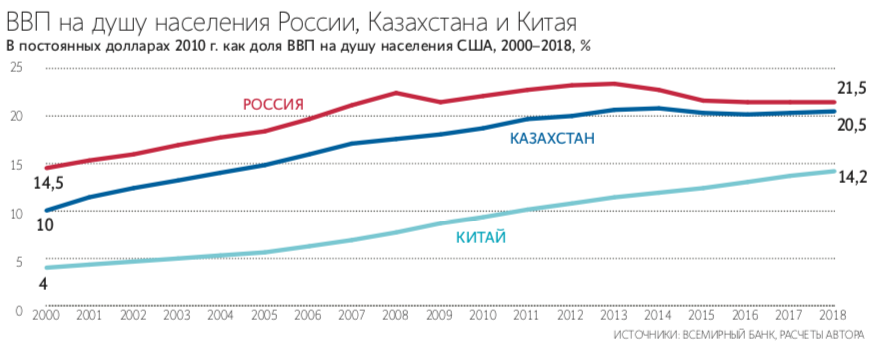
\includegraphics[width=0.68\textwidth]{img/1tbz.png}
    \end{center}
\end{wrapfigure}
\textbf{Авторитарный дедлок\footnote{deadlock}.}
Более жесткие деспотические режимы политологи называют «авторитарной гегемонией». На выборах здесь авторитарный лидер или правящая партия регулярно получают от 75 до 99\% голосов. Что, однако, свидетельствует не об их популярности, а о том, что они оказывают гораздо более систематическое давление на оппозицию, независимые СМИ и нелояльные элитные группы, т.е. отличаются от предыдущего типа резко возрастающим уровнем репрессивности. Встречаются они сегодня почти исключительно в Азии, Африке и бывшем СССР.

Как показывает опыт ряда азиатских стран, эволюция режима от первого типа ко второму часто происходит на фоне ухудшения экономической динамики. По мере того как экономика играет все меньшую роль в обеспечении легитимности и устойчивости режима, все большую роль начинают играть две другие опоры: репрессии и идеология. В информационной политике режим переходит от фильтрации и ограничения информации к агрессивной пропаганде. Начинаются систематические преследования гражданского активизма, появляются нормы, позволяющие в уголовном порядке преследовать за слова, криминализуется уличная активность граждан.

Именно переход от режима конкурентного авторитаризма к авторитарной гегемонии составил политическое содержание последнего путинского периода --- с 2013 по 2019 г. А геополитическая конфронтация выступила в качестве той идеологической рамки, которая легитимирует возрастающую репрессивность.

Хотя Россия выглядит сегодня гораздо более авторитарной страной, чем в 2012 г., этот переход, видимо, следует считать пока \ed{незавершенным}{незавершенный}{incomplete, uncompleted, unfinished}.
Наверное, играют свою роль развитая социальная инфраструктура мегаполисов, уровень европеизированности элит, глубина проникновения интернета и социальных медиа. Ну, и разумеется, \ex{экономический застой}{economic stagnation}. Несмотря на это, Путин вряд ли оставит свои усилия по девестернизации России. И это бесплодное (в исторической перспективе) \ex{перетягивание каната}{tug of war} скорее всего останется главным сюжетом финальной фазы его политической карьеры.


\newpage
\section[Евгений Пригожин]{Пригожин Евгений Викторович*}

\textit{Бизнесмен, владелец группы «Конкорд» и ЧВК «Вагнер»}

\textit{Источник \url{https://www.rbc.ru/person/63d280069a79473d6f5e3ce6}}

\textbf{Молодость, образование, родители.} Евгений Пригожин родился в Ленинграде. Его мать Виолетта Кировна Пригожина была медиком и работала в больнице. Отец Виктор Евгеньевич Пригожин рано умер, и ребенка воспитывал отчим Самуил Жаркой. Будучи лыжным инструктором, Жаркой приобщил его к беговым лыжам. В 1977 году Пригожин окончил ленинградскую спортивную школу-интернат № 62 (ныне колледж олимпийского резерва № 1), где учился вместе с пловцом Владимиром Сальниковым и гимнастом Александром Дитятиным, которые впоследствии стали трехкратными чемпионами московской Олимпиады. После школы поступил в Ленинградский химико-фармацевтический институт, получил специальность «провизор-фармацевт». В 2018 году в одном из интервью он сообщал, что институт не закончил.

\textbf{За что сидел Пригожин.} Агентство «Росбалт» (Минюст включил его в реестр СМИ-иноагентов) сообщало, что в ноябре 1979 года Куйбышевский районный народный суд Ленинграда приговорил Пригожина к двум с половиной годам лишения свободы условно по обвинению в краже. По данным Forbes, в 1981 году Ждановский народный районный суд Ленинграда приговорил Пригожина по новым обвинениям в краже, мошенничестве, вовлечении несовершеннолетнего в преступную деятельность и разбое к 13 годам колонии. В 1988 году Пригожин был помилован.

\textbf{Ресторатор, бизнес, карьера.} В 1990 году он стал заниматься бизнесом, начав с продажи хот-догов. Как пишет Forbes, этот бизнес он открыл вместе с отчимом, и часть производства находилась в квартире Пригожина. «Горчицу к хот-догам замешивали прямо у меня на квартире. [...] Приходилось платить бандитам с каждого ларька по \$100», — приводит издание его слова.

В 1991–1997 годах Пригожин управлял сетью частных продовольственных магазинов «Контраст», в 1995 году открыл бар-магазин «Винный клуб» на Васильевском острове в Санкт-Петербурге. В 1996 году, после знакомства с ресторатором Тони Гиром, открыл первый «элитный» ресторан города — «Старая таможня», после появились «Русский китч», «Семь сорок» и «Строгановский дворец».
В том же 1996 году Пригожин основал компанию «Конкорд кейтеринг».

В 1997 году Пригожин открыл ресторан на теплоходе, который получил название New Island и стал на тот момент самым дорогим рестораном Петербурга.
В 1999 году в New Island ужинали премьер-министр Сергей Степашин и директор-распорядитель МВФ Мишель Камдессю.

Пригожин продолжал заниматься розничным фастфудом и с 2002 по 2012 год развивал в Петербурге сеть кафе-блинных под придуманным им названием «Блин! Дональт's». Заведения сети позиционировались как социально значимые, с дешевой едой для местных жителей, блюда в меню получали необычные названия — в частности, там был сэндвич «квадрососисон». Бизнесмен планировал открыть до 20 кафе, однако к 2008 году открылось лишь десять, а с 2009 года компания Пригожина начала закрывать рестораны, последний из которых закончил работать в 2012 году. Сеть фактически послужила основой для создания Пригожиным в дальнейшем формата комбинатов питания. В 2016 году, как писал тогда РБК, Пригожин фактически стал монополистом на рынке школьного питания в Москве.

Строительным бизнесом Пригожин начал заниматься в 2000-х годах в Петербурге. В частности, как писала «Фонтанка», «Конкорд» в районе Лахты построил жилой комплекс «Северный Версаль» из 45 трехэтажных домов в стиле архитектуры Петербурга XVIII—XIX веков.

В 2008 году компания Пригожина ООО «Конкорд менеджмент и консалтинг» (входит в группу «Конкорд») получила участок рядом с парком 300-летия Петербурга для строительства Центра водного туризма. В 2011 году компания обратилась в суд, заявив, что городские власти затягивают выделение участка. В 2012 году суды трех инстанций подтвердили права инвестора. К марту 2016 года компания возвела на участке комплекс «Лахта Плаза» из шести жилых зданий общей площадью 41,9 тыс. кв. м.

В 2010 году компания, принадлежащая жене Пригожина, арендовала в центре Петербурга Дом торгового товарищества «Братья Елисеевы», в котором после реконструкции открылся «Магазин купцов Елисеевых». Летом 2016 года компания добилась права приватизировать здание за 740 млн руб.

Компания Пригожина также сотрудничала с Минобороны: за период c конца 2014 года по середину 2015-го структуры «Конкорда» выиграли тендеры на 10,3 млрд руб. на уборку в казармах и учебных заведениях оборонного ведомства, подсчитывал тогда РБК. Связанная с Пригожиным компания «Мегалайн» получила в 2015 году контракт на 3,3 млрд руб. на строительство военной базы в Валуйках в Белгородской области, она же выиграла на конкурсе контракт на 161,6 млн руб. на строительство военного городка в Омской области. В том же году несколько связанных с Пригожиным компаний выиграли тендеры на жилищно-коммунальное обслуживание военных городков в нескольких областях страны.

\textbf{Фабрика троллей Пригожина.} Имя Пригожина связывают с созданным летом 2013 года Агентством интернет-исследований, которое в прессе называли «фабрикой троллей». В США эту структуру обвиняли во вмешательстве в выборы. Сам Пригожин долгое время это опровергал. В феврале 2023 года бизнесмен заявил, что придумал Агентство интернет-исследований. «Я его создал, я им управлял длительное время. Создано оно было для защиты российского информационного пространства от хамской агрессивной пропаганды антироссийских тезисов со стороны Запада», --- заявил Пригожин.

В 2017 году стало известно о создании структурами Пригожина «фабрики медиа», в которую вошли Федеральное агентство новостей, а также другие связанные с ним издания, в частности «Политика сегодня», «Экономика сегодня» и «Народные новости». Согласно расследованию журнала «РБК», к февралю 2017 года ежемесячная аудитория изданий «фабрики медиа» достигла 36 млн человек, превысив аудиторию агентства «РИА Новости» и «Комсомольской правды». Вскоре эти издания вошли в медиагруппу «Патриот».

В США Пригожина обвинили во вмешательстве в выборы 2016 года и в политический процесс. В феврале 2021 года ФБР назвала Пригожина в числе 13 россиян, которые объявлены в розыск за вмешательство в выборы президента США. Ведомство предложило вознаграждение в размере до \$250 тыс. за сведения, которые помогут заключить бизнесмена под стражу. Пригожин назвал действия бюро «шоу с розыском, как в старые ковбойские времена», и потребовал удалить с сайта ФБР объявление о вознаграждении за информацию о нем.

\textbf{ЧВК Вагнер Евгения Пригожина.} Пригожин — основатель частной военной компании (ЧВК) «Вагнер». Журнал «РБК» писал о полигоне у населенного пункта Молькино в Краснодарском крае, который начал использоваться, предположительно, для подготовки бойцов ЧВК в середине 2015 года. В октябре 2015-го о наборе добровольцев в состав ЧВК и участии ее бойцов в наземных операциях в Сирии, а также в конфликте на территории Луганской и Донецкой народных республик сообщала «Фонтанка». ЧВК получила название «Вагнер» в 2014 году по позывному первого командира подразделения, офицера запаса Дмитрия Уткина.

В США и Евросоюзе заявляли о действиях ЧВК «Вагнер» также в Ливии, ЦАР, Судане, Мозамбике и Мали. Госдепартамент заявлял, что деятельность «Вагнера» в Африке мешает работе миротворцев ООН на континенте.

В июле 2018 года в ЦАР для съемок фильма о деятельности ЧВК направились журналист Орхан Джемаль, оператор Кирилл Радченко и режиссер Александр Расторгуев. По пути к месту съемок их машину атаковали неизвестные вооруженные люди. Журналисты погибли, с места убийства россиян пропали деньги, техника и документы.

США и Евросоюз обвиняли ЧВК «Вагнер» в нарушении прав человека на Ближнем Востоке и в Африке и ввели против компании санкции, которые были ужесточены после начала российской спецоперации на Украине. Санкции были введены в 2016 году и против Пригожина, которого обвинили в связях с ЧВК.

Пригожин долгое время отвергал связь с ЧВК, заявляя, что «крайне удивлен самим фактом существования данной компании и не имеет к ее деятельности никакого отношения». Однако в сентябре 2022 года признался, что именно он является ее создателем. В конце октября 2022-го бизнесмен заявил о создании в Санкт-Петербурге «ЧВК Вагнер Центра», в котором «смогут работать специалисты в области оборонных и информационных технологий с целью повышения обороноспособности России».

\textbf{ЧВК Вагнер на Украине.} Соединения ЧВК активно участвовали в боевых действиях на Украине, в частности под Артемовском (украинское название — Бахмут) и в Соледаре.

Летом 2022 года начали появляться сообщения о посещении Пригожиным тюрем с целью вербовки заключенных в ряды «Вагнера».

\begin{fancyquotes}
    Те, кто не хочет, чтобы воевали ЧВК, заключенные, кто рассуждает на эту тему, кто ничего не хочет делать и в принципе кому эта тема не нравится, детей своих на фронт отправьте. Либо ЧВК и зэки, либо ваши дети — решайте сами

    \begin{flushright}
        Пригожин в сентябре 2022 года\\
        о вербовке заключенных для участия в спецоперации на Украине
    \end{flushright}
\end{fancyquotes}

В ноябре 2022 года телеграм-канал GREY ZONE, который в Совете по правам человека связали с ЧВК «Вагнер», опубликовал видео убийства мужчины, которого назвали бывшим бойцом ЧВК Евгением Нужиным, участвовавшим в спецоперации. На видео мужчина называет свое имя и дает интервью украинским журналистам, заявляя, что добровольно перешел на сторону Киева. Затем Нужина показывают в темном помещении, и его голова примотана к кирпичам скотчем. Мужчина рассказывает, что 11 ноября 2022 года он находился на улице Киева, где получил удар по голове, в результате чего потерял сознание. «Очнулся в этом подвале, где мне сообщили, что меня будут судить», — говорит мужчина на записи, после чего получает удары кувалдой по голове.

После пленения Нужин в интервью украинскому журналисту Юрию Бутусову рассказал, что сам родом из города Перевоз в Нижегородской области и в 1999 году был осужден на 24 года лишения свободы за убийство человека, а затем из-за неудачного побега ему добавили еще четыре года.

Пригожин, комментируя видео, назвал его «прекрасной режиссерской работой». «Что касается окувалдованного, то в данном шоу видно, что он не нашел счастья в Украине, а встретился с недобрыми, но справедливыми людьми», — отметил он.

Позже Пригожин обратился к генпрокурору с просьбой провести доследственную проверку по факту убийства Нужина. 15 ноября уполномоченная по правам человека Татьяна Москалькова заявила РБК, что следственные органы занялись проверкой.

23 ноября Европарламент принял резолюцию, в которой Россия называется страной — спонсором терроризма в связи с военными действиями на Украине. В документе также содержался призыв к странам ЕС признать ЧВК «Вагнер» и входящий в Росгвардию 141-й полк имени Ахмата Кадырова террористическими организациями. После этого пресс-служба Пригожина сообщила, что тот отправил в Европарламент в футляре из-под скрипки «брендированную кувалду [...] с, вероятнее всего, бутафорскими следами крови».

В январе 2023 года США объявили ЧВК «Вагнер» транснациональной преступной организацией. В ответ Пригожин написал письмо в Белый дом с просьбой прояснить, какие преступления совершала эта организация.

Пригожин неоднократно критиковал власти Петербурга и губернатора Александра Беглова. В июле 2022 года он обвинил губернатора в создании помех для бизнеса, после того как структуры, связанные с предпринимателем, не получили контракт на обустройство территории «Горская» и разработку доверили другой компании, несмотря на инвестиционное соглашение. В администрации Петербурга эту точку зрения назвали частным мнением бизнесмена, отстаивающего свои интересы. Беглов заявлял, что действия правительства Петербурга вызывают критику со стороны некоторых «богатых людей, влиятельных людей, которые могут налом проплачивать определенные вещи», не уточняя, кого конкретно имеет в виду. В Кремле, комментируя подобные высказывания Пригожина, заявили, что тот, как предприниматель, «болеет душой за то, что происходит».

\textbf{Призыв к мятежу и уголовное дело.} Вечером 23 июня Пригожин заявил, что российские военные нанесли удар по лагерю ЧВК «Вагнер», в результате чего погибло «погибло огромное количество бойцов». Он обвинил в этом «военное руководство» и пообещал ответ. Позже пресс-служба основателя ЧВК распространила заявление Пригожина, в котором он уточнил, что его намерение «ответить» --- это «не военный переворот, а марш справедливости».

Минобороны утверждения Пригожина опровергло, назвав их «информационной провокацией». В ведомстве подчеркнули, что вооруженные силы «продолжают выполнение боевых задач на линии соприкосновения с вооруженными силами Украины».

Вскоре ФСБ и Генпрокуратура отчитались о возбуждении уголовного дела против Пригожина по статье 279 Уголовного кодекса по факту организации вооруженного мятежа. В ФСБ заявили, что заявления и действия Пригожина фактически являются призывами к началу вооруженного гражданского конфликта на территории и призвали бойцов ЧВК задержать своего лидера. «Призываем бойцов ЧВК не совершать непоправимой ошибки, прекратить любые силовые действия против российского народа, не выполнять преступные и предательские приказы Пригожина, принять меры к его задержанию», — говорилось в заявлении.

Обратился к бойцам ЧВК и генерал Сергей Суровикин. «Я обращаюсь к бойцам и командирам ЧВК «Вагнер». Мы вместе с вами прошли трудный тяжелый путь. Мы вместе с вами воевали, шли на риски, несли потери, вместе побеждали. Мы одной крови. Мы воины... Пока не поздно, нужно и необходимо подчиниться воле и приказу всенародно избранного президента. Остановить колонны, вернуть их в пункты постоянной дислокации», — сказал он в видео, опубликованном военкором Андреем Руденко.

Вечером 24 июня президент Белоруссии Александр Лукашенко сообщил, что провел переговоры с Евгением Пригожиным, они достигли договоренности об остановке движения бойцов ЧВК по территории России. Глава Белоруссии заявил, что бойцам Пригожина дадут гарантии безопасности. Основатель «Вагнера» заявил, что разворачивает свои колонны и уходит в полевые лагеря «согласно плану».

27 июня дело о мятеже было закрыто. Лукашенко заявил, что Пригожин приехал в Белоруссию. «Как я и обещал, если вы хотите какое-то время у нас перекантоваться и прочее, мы вам поможем. Естественно, за их счет», — заявил президент Белоруссии.

Путин заявил, что «организаторы мятежа, предали свою страну и народ». Он также заявил, что содержание ЧВК «Вагнер» полностью обеспечивалось государством. По словам президента, с мая 2022 года по май 2023-го на денежное содержание и стимулирующие выплаты ЧВК государство заплатило 86 млрд и 262 млн руб. «При всем том, что само содержание «Вагнера» было на плечах государства, за год собственник компании «Конкорд» через «Военторг» получил, заработал от государства, поставляя продукты питания и оказывая услуги по питанию в армии, заработал 80 миллиардов рублей», — сказал Путин. Он добавил, что надеется на то, что «в ходе этих работ никто ничего не украл или, скажем так, украл поменьше». По его словам, с этим еще предстоит разобраться.

\textbf{Катастрофа самолета в Тверской области.} Вечером 23 августа 2023 года в Тверской области разбился самолет Embraer Legacy, совершавший рейс Москва — Санкт-Петербург. Как сообщили в МЧС, на борту находились 10 человек, все они погибли. В Росавиации сообщили, что Пригожин был в списке пассажиров самолета. Позже ведомство уточнило, что, по данным авиакомпании, которой принадлежал самолет, бизнесмен действительно был на борту. Также там находится командир ЧВК «Вагнер» Дмитрий Уткин.

Как 24 августа сообщил Владимир Путин, Пригожин в день авиакатастрофы вернулся из Африки. Президент также рассказал, что знал бизнесмена «с начала 90-х годов». «Это был человек сложной судьбы, и ошибки у него были серьезные в жизни, добивался он результатов нужных — и для себя, и для, когда я его просил, для общего дела, как в эти последние месяцы. Он был талантливый человек, талантливый бизнесмен», — добавил Путин.

27 августа СК сообщил, что экспертиза подтвердила гибель Пригожина и остальных пассажиров самолета.

\textbf{Личная жизнь, жена, дети.} Пригожин женат, у него трое детей. Члены семьи Пригожина, в том числе его дети Полина и Павел, в 2022 году попали под санкции ряда западных стран. Под санкции ЕС и Канады также попала мать Виолетта Пригожина (1939 г.р.). Но в марте 2023-го она смогла добиться аннулирования ограничений, введенных против нее Евросоюзом. Суд ЕС установил, что она не владеет компанией «Конкорд Менеджмент и Консалтинг», как считал Брюссель, а родственных связей для включения в санкционный список недостаточно.

В 2003 году Пригожин вместе с детьми Полиной и Павлом написал книгу сказок «Индрагузик», в которой описана сказочная страна Индрагузия.

В сентябре 2022 года Пригожин на странице своей пресс-службы в соцсети «ВКонтакте» сообщил, что его сын в возрасте 18 лет прошел службу в вооруженных силах и через месяц после армии «поехал на войну в Сирию». «С тех пор он постоянно находился и находится в горячих точках в составе ЧВК «Вагнер», где и получил свой первый Черный крест (награда ЧВК. — РБК)», — говорилось в сообщении.

Пригожин награжден орденом «За заслуги перед Отечеством» IV степени «за достигнутые трудовые успехи, значительный вклад в социально-экономическое развитие Российской Федерации, заслуги в освоении космоса, гуманитарной сфере, укреплении законности, активную законотворческую и общественную деятельность, многолетнюю добросовестную работу», и медалями ордена «За заслуги перед Отечеством» I и II степеней. Также в публичных источниках есть фотографии Пригожина со звездами Героя России, Героя Донецкой и Луганской народных республик. В Кремле на вопрос о присвоении Пригожину звания героя закрытым указом президента заявили лишь, что все открытые указы публикуются.

\newpage
\section{Еда на планете становится дефицитом}

\textit{Что будет с ценами на продукты в России и мире}

\textit{Почему продукты на планете постоянно дорожают}

\textit{Источник \url{https://www.kp.ru/daily/27547.5/4814137/}}

Продовольственный кризис \ex{разворачивается}{is unfolding} на нашей планете прямо сейчас. Трудно в это поверить, глядя на переполненные полки супермаркетов. Но нехватку еды, по данным ООН, ощущают на себе уже около 2 млрд человек в 80 странах. А около 20 тысяч человек ежедневно умирает от голода и его последствий.

Последний резкий рост цен на продовольствие случился в 2020 - 2022 годах. И это был уже третий \ex{скачок}{jump} за последние 15 лет. В первой половине 2023 года цены вроде пошли вниз, но в июле --- новый рост. Так в чем причины нехватки еды на планете?

\textbf{Причина № 1. Конфликты и войны.} Это одна из главных причин: 70\% голодающих живут на территориях, где происходят боевые столкновения. И \ed{нынешнее}{нынешний}{present, current} вооруженное \ex{противостояние}{confrontation} на Украине тоже ударило по самым чувствительным точкам --- поставкам энергоносителей, удобрений и сельхозпродукции.

До начала боевых действий Россия и Украина экспортировали на мировые рынки значительные доли пшеницы (18\% и 10\%), ячменя (14\% и 12\%), \ed{подсолнечного масла}{подсолнечное масло}{sunflower oil} (26\% и 37\%). После начала кризиса объемы экспорта сельхозпродукции с Украины сократились на 30 - 40\%. Странам Европы, Азии и Африки пришлось искать новых \ed{поставщиков}{поставщик}{supplier} и выстраивать новые пути доставки, что привело к росту цен.

\textbf{Причина № 2. Природные катаклизмы.} Особенно от этого страдают жители Африки и Юго-Восточной Азии. В 2021 - 2022 годах дефицит осадков здесь достигал 80\%. Грустный итог: с середины 2021 года по апрель 2022-го в Кении и Эфиопии погибло около 3 млн голов скота. Похожая ситуация в Сомали.

А в западной части континента все наоборот: наводнения уничтожают пахотные земли. По оценке ООН, производительность сельского хозяйства в Африке по итогам 2022 года снизилась на 34\%.

Страдают от аномалий погоды Индия, Китай, Южная Америка. Постоянно дают о себе знать течения Эль-Ниньо и Ла-Нинья: температура воды в экваториальной части Тихого океана меняется, влияя на осадки в Азии и Южной Америке.

Не жалеет погода и США. Из-за жары 2022 года урожай пшеницы в Америке сократился вдвое, а на юге Европы погодные аномалии принесли убытки на миллиарды евро...

\textbf{Причина № 3. Энергетический кризис.} Для производства, доставки, упаковки, хранения продуктов нужна энергия --- газ, нефть, электричество. А газ и нефть резко дорожали в 2021 - 2022 годах (цена на голубое топливо взлетала в несколько раз). Последствия этого скачка мир ощущает до сих пор.

\textbf{Причина № 4. Нехватка удобрений.} Современное сельское хозяйство \ex{немыслимо}{unthinkable} без минеральных удобрений, а они постоянно дорожают. С 2022 года этот рынок залихорадило снова: сказались \ed{перебои}{перебой}{interruption} с поставками из России, введение экспортных квот Китаем и подорожавший в 2022 году природный газ --- ключевой компонент при изготовлении азотных удобрений. Проблемы с газом заставили многие страны сократить собственное производство.

Итог --- цены на отдельные виды удобрений подскочили в три раза, что сразу ударило по стоимости продуктов. Нехватка удобрений наверняка скажется и на урожайности.

На мировые цены влияет множество факторов. Стоимость отдельных продуктов может не только расти --- бывает, что цены снижаются. Но, как шутят эксперты, если цены падают на биржах, они не падают на наших кухонных столах. Ведь стоимость сельхозтоваров формируется главным образом после того, как они покидают фермы. Речь о затратах на энергию, обработку, упаковку, доставку, рабочую силу... И каждая из этих позиций из года в год прибавляет в цене. В итоге по пути в магазин продукты дорожают в 2 - 3 раза, а то и больше.

В этом году быстрее других продуктов дорожают зерно, рис, какао и апельсины. Давайте выясним, почему.

\textbf{Нерациональное зерно.} Мировой рынок зерновых \ex{трясет}{is shaking}. В начале марта цены на пшеницу достигали исторического максимума --- \$12,09 за бушель (единица объема для измерения зерна, один бушель равен в среднем 27,21 кг). Затем они падали, снова росли, особенно после того, как Россия вышла из «зерновой сделки». Напряжение между Россией и Украиной играет здесь важную роль, поскольку обе страны --- крупные поставщики этого продукта на мировой рынок.

Сейчас стоимость пшеницы на биржах упала до 6,5 доллара за бушель, но как цены поведут себя дальше, сказать трудно. С одной стороны, замедляется спрос на зерновые корма. С другой - к увеличению потребления зерновых ведет рост населения планеты.

Мировая торговля зерном к 2031 году должна вырасти на 15\%, а пшеница в общем объеме занимает около 40\%. И Россия останется одним из лидеров по экспорту пшеницы на мировой рынок (доля - более 20\%). Оптимизма добавляют и хорошие урожаи в нашей стране.

Сообщения о том, что в России из-за ситуации на зерновом рынке может подорожать хлеб, на днях опроверг Минсельхоз. Здесь уверили: обеспеченность России зерном намного превышает внутренние потребности. Поэтому рост цен на хлеб в этом году будет не выше общей инфляции (по плану --- не более 6,5\%).

\textbf{Рис --- благородное дело.} Цены на рис в этом августе достигли многолетних максимумов. Например, эталонный для экспортеров в Азии тайский белый рис стоил \$650 за тонну - это на 50\% больше, чем в августе прошлого года. Особенно быстро цена на рис стала расти с июля, после объявления Всемирной метеорологической организацией ООН о появлении Эль-Ниньо, вызывающего засухи.

Кроме того, недавно Индия --- крупнейший поставщик риса --- заявила о запрете экспорта 80\% этой продукции, чтобы сдержать рост внутренних цен на этот стратегический для страны товар. Временно запретили экспорт риса ОАЭ и Россия. Но стратегическим продуктом рис остается не только для Индии, а для 40\% населения Земли, особенно в Азии. Он обеспечивает базовое питание 3 млрд человек. И экономисты \ex{опасались}{they feared}, что осенью цены на рис могут вырасти вдвое к прошлому году.

России рост цен пока не грозит. Во-первых, наша страна сама выращивает рис. Его мы ежегодно производим больше миллиона тонн, и этого хватит, чтобы удовлетворить внутренний спрос. Во-вторых, правительство вовремя ввело ограничения на вывоз этого продукта из страны --- теперь у аграриев нет \ed{искушения}{искушение}{temptation} экспортировать рис, пользуясь выгодными для себя ценами.

\textbf{Чао, какао!} Какао-бобы, а точнее, какао-масло, которое из них производят, --- один из главных ингредиентов в производстве шоколада. Дефицит и подорожание какао приведет к росту цен на всю кондитерку.

Стоимость какао-масла выросла с начала года уже на 20\% и приблизилась к максимальному уровню за последние полвека, преодолев в июле \ed{отметку}{отметка}{mark} 3500 долларов за тонну. Причина --- плохая погода в Западной Африке. Ведь как раз на две страны этого региона --- Кот-д' Ивуар и Гану --- приходится 60\% мирового производства какао.

Основатель фабрики ShokoBox Андрей Шарков уверен, что повышения цен на шоколад не избежать и России. Причины -- \ex{подорожание}{rise in price, price hike} сырья на мировых рынках и ослабление рубля. Ведь наш шоколад производится из импортных компонентов.

\begin{fancyquotes}
    Думаю, что осенью нам следует ожидать роста цен на шоколадные изделия в среднем на 10\%, - рассказал Андрей Шарков «КП». - При этом их качество станет хуже.
\end{fancyquotes}

Многие производители попытаются компенсировать рост цен заменой натурального какао-масла дешевыми заменителями. Российский рынок не слишком требователен к качеству, но те, кто ценит настоящий шоколад, почувствуют разницу. И качественные продукты без заменителей подорожают еще больше. Мой прогноз --- на 20\%.

\textbf{Нету сладких апельсинов.} Бразилия была и остается крупнейшим мировым поставщик\'{о}м концентрата для производства апельсинового сока. Но в этом году в стране \ex{неурожай}{bad harvest, crop failure}, цены поползли вверх. Масла в огонь подлили неблагоприятная погода и плохой урожай цитрусовых в США, Мексике и Испании. В итоге за год стоимость фунта замороженного концентрата апельсинового сока выросла с 2 до 3 долларов.

В России цены на апельсины росли с 2020 года. А этим летом наши торговые сети столкнулись с их дефицитом, так что дорожать они, видимо, будут и дальше. Замороженный концентрат апельсинового сока уже подорожал в России на 30\%. Что неизбежно приведет к пропорциональному росту цен.

\textbf{В ТЕМУ}

\textbf{Пицца против окрошки}

\textbf{Национальные блюда тоже бьют по кошельку}

Официальные цифры инфляции не всегда отражают то, как ощущают на себе подорожание продуктов обычные граждане. В ЕС, например, продовольственная инфляция составляет порядка 12,5\%. Но если взять популярную в Италии пиццу «Маргарита», то ее цена в январе 2023-го, по данным Bloomberg, выросла к январю 2022 года на 25\%. Притом, что официальная инфляция в Италии за этот период составила 10,7\%. А все потому, что сильно взлетели цены на сыр и муку.

Похожая ситуация с национальным блюдом испанцев паэльей. Она за год подорожала на 19\% при общей инфляции в Испании 6\%. Сказался рост цен на оливковое масло, овощи и бобы.

На 20\% подорожал классический британский завтрак (сюда входят бекон, колбаски, яйца, тосты и напиток). Причина - рост цен на молоко, хлеб и яйца. Кстати, в США именно яйца рекордно взлетели в цене - в начале 2023 года они стоили на 60\% дороже, чем годом ранее.

А вот окрошка подорожала за год всего на 6\%. Виноваты в основном овощи. Редис подорожал к прошлому году почти на треть, огурцы - на 25\%, зеленый лук - на 5\%. Даже квас прибавил в цене 6\%. Зато картофель и яйца подешевели.

\textbf{ТОЛЬКО ЦИФРЫ}

29,3\% всего населения планеты испытывают умеренную или серьезную нехватку продовольствия.

Более 345 млн человек столкнутся в 2023 году с «высоким уровнем отсутствия продовольственной безопасности». По сути --- будут \ed{недоедать}{недоедать/недоесть}{to be undernourished, to not eat enough}.

14 из 15 стран с наибольшим отсутствием продовольственной безопасности находятся в Африке.

По данным ФАО ООН и Всемирной продовольственной программы ООН.


\clearpage

% \chapter{Война и мир}

\section{Что ждет россиян во время частичной мобилизации?}
\textit{Источник: \url{https://lenta.ru/articles/2022/09/21/ukaz/}}

\textit{Ответы на главные вопросы}

Президент России Владимир Путин 21 сентября 2022 года объявил о введении в России \ed{частичной}{частичный}{partial} мобилизации. По его словам, призыву на военную службу подлежат граждане, состоящие в запасе, и прежде всего те, кто служил в армии. Кто теперь подлежит призыву, кто имеет право на \ed{отсрочку}{отсрочка}{delay; postponement}, каков порядок мобилизации — в этих вопросах разбиралась «Лента.ру».

\ed{Указ}{ук\'{а}з}{decree} «Об объявлении частичной мобилизации в Российской Федерации» опубликован на сайте Кремля в среду, в 9 часов 20 минут.

«Объявить с 21 сентября 2022 года в Российской Федерации частичную мобилизацию», — сообщается в первом пункте документа, подписанного президентом России Владимиром Путиным.

Во втором пункте указано, что мобилизованные граждане получат статус военнослужащих-контрактников с денежным содержанием соответствующего размера. Увольнение из рядов мобилизованных предусмотрено только по возрасту и по состоянию здоровья.

Правительству поручено финансировать мероприятия по проведению частичной мобилизации, главам регионов — обеспечить призыв находящихся в запасе граждан.

\textbf{Сколько человек призовут?}

Согласно заявлению главы Минобороны Сергея Шойгу — 300 тысяч. Это примерно 1,1 процента от общего мобилизационного ресурса России, который, по словам министра, составляет почти 25 миллионов человек. Для каждого региона количество подлежащих мобилизации будет определяться отдельно.

\textbf{Кого призовут в первую очередь?}

По словам Шойгу, на военную службу по мобилизации будут призваны те, кто отслужил в армии, имеет военно-учётную специальность и соответствующий опыт. Перед отправкой в части они пройдут обязательную дополнительную подготовку.

\ed{Полковник}{полковник}{colonel (army)} \explain{в отставке}{retired} Виктор Баранец считает, что первыми под мобилизацию попадут резервисты, которые каждый год по указу президента призывались на военные сборы, стреляли, водили танки и наводили ракеты. Кроме того, будут призваны люди, по разным причинам уволенные с контрактной службы, а также молодые офицеры.

«Резервисты -- это \explain{военнообязанные}{conscripts; liable for military service} граждане государства, которые подлежат мобилизации при необходимости, -- рассказал в свою очередь «Ленте.ру» \explain{судь\'{я}}{judge} в отставке Владимир Комсолев. —- В нашем случае это лица, прошедшие службу и имеющие достаточную подготовку. Они заключили контракт о пребывании в резерве и получают за это деньги. Раз в год резервисты выезжают на военные сборы, раз в месяц участвуют в занятиях».

Юрист Артем Мугунянц в разговоре с «Лентой.ру» отметил, что тех, кто пользовался отсрочкой в период с 18 до 27 лет и не служил, мобилизация, вероятно, не коснётся.

«Мобилизации подлежат только те, кто служил в армии либо офицером, либо проходил срочную службу, либо был контрактником\footnote{Only those who served in the army either as an officer, or did military service, or were a contract soldier \textit{are subject to} mobilization}. — пояснил эксперт. — Можно предполагать следующее. Так как утверждается, что необходимо освобождать территории Украины, им потребуются \explain{наступательные войска}{offensive troops}: танкисты, \explain{морская пехота}{marines}, мотострелковые части. Эти части и войска могут потребоваться в большом количестве. Тех, кто служил в этих войсках, будут мобилизовать в первую очередь».

\textbf{Людей какого возраста могут призывать?}

Согласно статье 53 Федерального закона «О воинской обязанности и военной службе», все военнослужащие запаса делятся на три разряда. В случае мобилизации первым в ВС попадает первый разряд, затем — второй, третий — последним (подробнее о том, что значат категории запаса и категории здоровья — ниже).

По первому разряду призываются солдаты и низшие \ed{чины}{чин}{rank} в возрасте до 35 лет, младшие офицеры в возрасте до 50 лет (в третьем разряде верхние рамки для этих званий повышаются до 50 и 60 лет соответственно) и так далее. Представители генералитета подлежат мобилизации по второму разряду в возрасте до 70 лет.

В Госдуме заявили, что планируют призывать тех, кто попадает под первый разряд.

«Пока человек не снят с военного учёта, он может подлежать мобилизации, — пояснил «Ленте.ру» профессор кафедры уголовного права РГПУ имени А.И. Герцена Сергей Милюков. — Есть специальности в ближнем и дальнем тылу, где возраст не является большой \ed{пом\'{е}хой}{пом\'{е}ха}{hindrance}. Например, обязательно потребуются медики. Призванные врачи будут оказывать медпомощь в госпиталях в тылу. Для лечения и \ed{дол\'{е}чивания}{дол\'{е}чивание}{follow-up treatment} нужно привлечь санатории, как это было в Великую Отечественную войну. Непосредственно же в боестолкновениях должны участвовать более молодые люди».

\textbf{Что означают категории запаса и категории здоровья в военном билете? }

Существует пять категорий годности к военной службе. Их определяют исходя из показателей здоровья и записывают данные об этом в военном билете.
\begin{itemize}
    \item «А» — \explain{годен}{fit} к военной службе;
    \item «Б» — годен к службе с \ed{незначительными}{незначительный}{insignificant} ограничениями;
    \item «В» — ограниченно годен к военной службе;
    \item «Г» — временно не годен;
    \item «Д» — не годен к несению военной службы.
\end{itemize}
Группы здоровья «А», «Б» и «В» по федеральному закону \explain{подлежат}{are subject to} мобилизации.

Всех резервистов \ed{распределяют}{распределять}{distribute} по трем категориям в зависимости от возраста военнослужащего и полученного звания.

Первая категория — граждане, которых призывают в первую очередь в случае мобилизации. \explain{Речь идет о}{This is a very useful expression; it means ``this is about...''} военных, которые не получили офицерский чин (в том числе \ed{прапорщики}{прапорщик}{ensign} и мичманы) и не \explain{перешагнули}{stepped over} возрастной \explain{пор\'{о}г}{threshold} в 35 лет, а также о младшем офицерском составе до 45 лет (лейтенант, капитан). В данной категории числятся старшие офицеры до 50 лет (майор, \explain{подполковник}{lieutenant colonel}); полковники, капитаны 1 ранга до 55 лет; высшее руководство до 60 лет. Первым на службу должен прибыть офицерский состав высшего эшелона.

Вторая категория — военнообязанные старшей возрастной группы или те, кто не прошел в первую волну мобилизации по здоровью. В эту группу попадают солдаты, военнослужащие без офицерского звания в возрасте от 35 до 45 лет, младший руководящий состав от 45 до 50 лет и старшие офицеры от 50 до 55 лет.

Третья категория — военнослужащие, которых призывают только в том случае, если военные действия длятся больше года и необходимы дополнительные силы. Под эту категорию попадают \explain{рядовые}{privates} и \explain{матросы}{sailors}, прапорщики и мичманы самой старшей возрастной категории. Возраст низшего\footnote{низкий, низшего} офицерского состава этой категории до 55 лет, а для капитанов 2 и 3 ранга и подполковников — до 60 лет. В данной категории пребывают военнообязанные женщины в возрасте до 50 лет.

\textbf{Что такое мобилизационное предписание? }

Это документ, который выдается части запасников. Выдача мобилизационного предписания — это \explain{своеобразная}{peculiar, singular, sui generis} перепись военнообязанных лиц. Гражданин, который получил мобилизационное предписание, при объявлении мобилизации должен прибыть в указанное в нем место и срок без дополнительной \ed{повестки}{повестка}{subpoena, writ} и предупреждения.

Как \explain{утверждает}{claims} юрист Павел Чиков, во время мобилизации гражданам приходят повестки, как и в обычное время — лично в руки или под подпись. Повестку также могут вручить по месту работы.

Однако именно запасники, имеющие мобилизационные предписания, по статье 21 ФЗ «О мобилизационной подготовке и мобилизации в Российской Федерации» самостоятельно должны \explain{явиться}{show up} в военный комиссариат.

\textbf{Кто имеет право на отсрочку?}

Как следует из указа, подписанного Путиным, \ed{отсрочку}{отсрочка}{postponement} пол\'{у}чат работники оборонных предприятий. «\explain{Предоставить}{provide} гражданам Российской Федерации, работающим в организациях оборонно-промышленного комплекса, право на отсрочку от призыва на военную службу по мобилизации (на период работы в этих организациях). Категории граждан Российской Федерации, которым предоставляется право на отсрочку, и порядок его предоставления определяются правительством Российской Федерации», — говорится в документе.

Как следует из статьи 18 федерального закона о мобилизации, отсрочка также предоставляется:

\begin{itemize}
    \item временно \ed{негодным}{негодный}{ineligible, not qualified} к военной службе по состоянию здоровья;

    \item ухаживающим за близкими родственниками, которых больше некому содержать;

    \item многодетным родителям (тех, кто имеет на \ed{иждивении}{иждив\'{е}ние}{dependent} не менее четырех детей в возрасте до 16 лет или троих детей при условии беременности супруги сроком не менее 22 недель);

    \item родителям-одиночкам;

    \item членам Совета Федерации и депутатам Госдумы.
\end{itemize}

Другие категории военнообязанных, которым \explain{полагается}{depends, relies} отсрочка (бронь от призыва), еще не известны. Их определяет правительство России, напомнил пресс-секретарь президента Дмитрий Песков.

\textbf{Попадают ли под мобилизацию срочники и те, кто не служил в армии? }

По закону о мобилизации — не попадают. Из него следует, что в ряды вооруженных сил должны быть направлены «граждане, пребывающие в запасе, не имеющие права на отсрочку от призыва на военную службу по мобилизации».

По словам юриста Ольги Лютницкой, \explain{срочники}{conscript} не попадают под эту категорию, так как они еще не переведены в запас.

Если гражданин не служил, например, потому, что был ограниченно годен, но у него есть военный билет, то веротность его мобилизации есть, сказала она «Ленте.ру».

Юрист Мугунянц уточнил, что срочники уже являются военнослужащими по призыву. Задействовать их до объявления полной мобилизации и войны нельзя.

\textbf{Можно ли мужчинам теперь выезжать за границу? }

В Федеральном законе «О мобилизационной подготовке и мобилизации в Российской Федерации» говорится, что «гражданам, состоящим на воинском учете, с момента объявления мобилизации воспрещается выезд с места жительства без разрешения военных комиссариатов, федеральных органов исполнительной власти, имеющих запас».

Юрист Лютницкая утверждает, что пока по вопросу \ed{запрета}{запрет}{ban, prohibition} выезда мужчинам за границу нет никаких законодательных актов и комментариев. Поэтому прямо сейчас никаких ограничений для выезда не существует.

Юрист Мугунянц также отметил, что выезжать никому не запрещено: выезд закрывается только при полной мобилизации.

«Если же человека мобилизовали, то есть признали военнослужащим, дали мобилизационное предписание о том, что он должен явиться, то он действительно не может выехать в другую страну. Потому что он мобилизован», — уточнил эксперт.

При этом скорее всего человека не будут вносить в каике-либо базы, но гражданин должен \explain{учитывать}{take into consideration}, что выезд будет расценен как \explain{уклонение}{evasion} от армии, за которое возникнут соответствующие \explain{уголовные последствия}{criminal implications}.

Член Совета по правам человека при президенте России Кирилл Кабанов заявил, что для людей без повесток на руках юридического запрета на выезд за границу нет.

\textbf{Что ждет тех, кто по достижении 27 лет получил справку вместо военного билета?}

Те, кто не проходил службу в вооруженных силах \explain{без уважительной причины}{without good reason} (например, сознательно \ed{уклонялся}{avoided, dodged}), и по достижении 27-летнего возраста получил справку \explain{взамен}{instead of} военного билета, вероятно, не будут призваны во время частичной мобилизации, так как они тоже — не служившие люди, считает юрист Мугунянц.

«На данном этапе у них никаких проблем нет. Если объявят всеобщую мобилизацию, то [обладателей справок] будут призывать, как и всех. К ним будут применяться те же условия, как к людям, которые не служили, но имеют военный билет. То же касается и тех, кто вообще не имеет никаких документов [подобного рода]. Важно, что они находятся в мобилизационном возрасте и подпадают под [всеобщую] мобилизацию».

По российскому законодательству, обладатель справки не может быть принят на государственную службу, в остальном его права не отличаются от прав владельца военного билета.

\textbf{\explain{Затрагивает}{affects} ли мобилизация женщин?}

По закону, мобилизация граждан, пребывающих в запасе, \explain{предполагает}{suggest} возможность призыва на военную службу медработников женского пола в возрасте до 45 лет. У них на руках есть военные билеты — медработники получают их после учебы.

Адвокат Владимир Шелупахин объяснил «Ленте.ру», что призыв состоящих на воинском учете женщин предполагается только в третью очередь, то есть после мужчин в возрасте 35-45 лет, в том числе граждан, пребывающих в запасе, но годных к военной службе с незначительными ограничениями (категория «Б») или ограниченно годных к военной службе (категория «В»).

«\ed{Вовсе}{вовсе}{at all} \explain{освобождаются}{released} от службы матери-одиночки и многодетные матери», — добавил юрист. Кроме того, на женщин распространяются и другие отсрочки, описанные в федеральном законе.

\textbf{Могут ли повестки приходить через «Госуслуги»?}

По официальной информации — нет. О возможной отправке повесток через сервис \ed{Госуслуг}{Госуслуги}{public services} 21 сентября написал Telegram-канала Baza. По информации издания, всем, кого собираются призвать, придет уведомление в аккаунте Госуслуг дополнением к обычным повесткам через почту.

Однако в Минцифры почти сразу это \explain{опровергли}{refuted}. «В связи с появившимися в соцсетях публикациями о том, что электронные повестки в рамках частичной мобилизации будут \explain{рассылаться}{be sent out} через Госуслуги, сообщаем, что таких планов нет. Необходимая законодательная база для этого отсутствует», — говорится в Telegram-канале министерства.

\newpage
\section{Таких замученных людей я раньше не видел*}

\textit{Рассказ россиянина, который несколько суток пытался уехать в Казахстан }

\textit{Источник: \url{https://baza.io/posts/4250c126-5344-458d-af97-21179596c136}}

Сутки на жаре и холоде, драки, голод и бессонница. Со всем этим столкнулся Александр, который после объявления о «частичной мобилизации» решил уехать на машине в Казахстан. Однако там его, как и тысячи других россиян, встретил своеобразный тест на выживание и целый ряд гуманитарных проблем.

Это детальный рассказ Александра о том, что сейчас происходит на границе с Казахстаном в Астраханской области.


\textbf{Добраться до границы}

Мчались к границе под Астраханью в режиме аврала: за ночь собрали чемоданы, бросили ключи от квартиры с котом друзьям и полетели в Волгоград, так как только туда в эти дни были нормальные цены на билеты. Самолёт был полностью забит мужчинами. Когда заходил, услышал, как одна бортпроводница шепнула другой насчёт пассажирки: «О, девушка, ничего себе! Впервые за два дня».

Уже в самолёте стало ясно: ехать, как мы планировали, на поезде до Астрахани очень долго, и потому прямо в аэропорту взяли таксиста. Спросили, за сколько он довезёт до границы под Астраханью, и он, назвав сумму в 15000, сразу получил её в руки. Мы гнали больше ста весь путь. В какой-то момент водитель даже чересчур заспешил и чуть не размазал нас по встречной фуре.

Остановились только один раз — на пустынной заправке у трассы. Там был заправщик, который принялся нам угрожать и затевать драку из-за того, что мы бежим из страны. Мы ничего ему не говорили, но ему было очевидно, что мы москвичи, так как он обронил «из-за таких, как вы, у меня всех братьев забрали».

Обидно было, что он именно нас в этом обвиняет, а не власть. Но вместе с тем жалко парня: многим очевидно, что в сёлах больше пропорции набора.


\textbf{Звёзды и безысходность под Астраханью}

Подобрались к границе Астрахань — Атырау с наступлением темноты, тогда длина пробки до КПП была уже 14,9 километра. Там уже царила анархия: нам с ходу предложили купить велосипед за 50000 рублей, на котором можно было проехать границу. Далее следовал жуткий марш-бросок в кромешной тьме с чемоданами под дождём в дикий холод: вместе с тьмой на пробку опустилась осенняя прохлада и ливень.

Мы прошли вместе с чемоданами около 8 километров, разглядывая, как люди друг с другом ругаются из-за мест, как плачут уставшие дети в машинах, как кричат кошки в переносках. Люди пытались лечь спать в совершенном аду. Над нами, стоит отметить, висело фантастически красивое звёздное небо: в радиусе километров не было огней, и это был фантастический вид на звёзды. Но вместе с тем впервые пришло отчаяние: стало понятно, что выжить тут будет нереально.

Вокруг сновали люди на велосипедах с подвязанными к спине чемоданами, люди на гироскутерах, самокатах, местная банда бородатых наглецов, отжимавших места поближе к границе на продажу, и огромная, невообразимая по длине пробка из легковых и большегрузных машин, у которой не было конца. Спустя два часа такого движения, не найдя конца очереди, мы устали смертельно, и пришло понимание: либо мы сейчас едем в аэропорт и домой, либо должны немедленно устроиться на ночлег. Я был замерзший, мокрый и абсолютно раздавленный безысходностью.

И тут я увидел паренька лет 20, который ехал один в этой пробке на своей машине. Ходили слухи, что пробку на машине можно преодолеть только за сутки-полтора, и я удивился: как он в одиночку, без смены собирался ехать такой период времени без остановки? Мы предложили ему за деньги взять нас до границы, пообещав подменять за рулём для сна. Парень согласился, и мы залезли в машину. Боже, как было уютно и тепло после холодной дождливой улицы! Мы часа три-четыре ехали с ним, стараясь лавировать между дальнобойными машинами, которые пытались блокировать дорогу бомбилам, занимающим места. При этом мы весело болтали за жизнь. Стало понятно, что компания приятная.

Я чувствовал, что дико устал. Время уже было около часа ночи, как вдруг движение встало. Перед нами была вереница дальнобойщиков, уходящая в бесконечную даль, и мы в ожидании, когда вновь начнётся движение, заглушили двигатель и в какой-то момент уснули.


\textbf{«Голодные игры»}

Я проснулся спустя пару часов: было холодно даже внутри машины, хотя спал я в куртке. Парень, который нас взял, курил возле авто, закутанный во всю одежду, что у него была. Мы стояли окружённые со всех сторон дальнобойщиками, которые спали в кабинах. А вокруг был шум двигателей. Казалось, все едут, и только мы стоим в своём маленьком дальнобойном ряду.

Парень сходил на разведку и вернулся с криком «Погнали!». На часах было только 4 утра, и тьма была непроглядная. Мы очень аккуратно вылезали между дальнобойщиками на обочину и, когда выехали, увидели сцену из какого-то плохого спин-оффа фильма «Голодные игры»: сотни автомобилей носятся по полю, пытаясь обогнать друг друга в пробке на дороге и влезть где-то ближе к первому блокпосту ГИБДД.

Мы вместе со всеми выехали на поле и оказались в абсолютной мясорубке: ночь, вой моторов и сотни водителей, выдавливающих друг друга с дороги в кювет. Уже не знаю, как у паренька это вышло, но благодаря своей наглости и терпению он нашёл небольшой перекрёсток с просёлочной дорогой, чтобы вклиниться, и мы заняли позицию до рассвета.


Рассвело к шести, и на перекрёстке появился сотрудник ГИБДД. Он пытался разрулить весь тот кошмар, который произошёл за предрассветные часы. Водителей, ждущих в пробке уже сутки, это злило: кто-то за ночь влез без очереди из-за дальнобойщиков, которые заблокировали поток в знак отместки за потерянное время. Теперь такие водители не давали сотруднику ГИБДД пропускать влезшие с обочины машины.

Инспектор был абсолютно уставший и измождённый и в какой-то момент просто ушёл, оставив всё это дело жить своей жизнью. А жизнь была такая: пока на горке совершали намаз мусульмане, семьи с детьми пытались умыть уставших и невыспавшихся детей, а кто-то гулял с собакой, привезённой с собой в этот кошмар.

«Нам тут не влезть», — хмуро сказал наш водитель, и мы пошли искать сообщников на прорыв. Картина открывалась жуткая. Поговорив с окружающими, мы узнали, что люди, стоявшие в честной пробке, провели здесь уже сутки, тогда как наш маршрут занимал около 10 часов. Многие были с детьми, пожилыми родителями, животными. Кто-то из них набрал попутчиков. Но всех объединяло одно: все они, так же как и мы, ночью были заблокированы колонной дальнобойщиков.

Услышав шум машин и оскорбившись такой наглостью, водители бросились объезжать их по полям, перемешивая все очередности. Этот перекрёсток был всего в 5 километрах от границы.


\textbf{Банка майонеза, драки и ФСБ}

В пробке было много машин с Северного Кавказа: с номерами из Дагестана, Чечни, Ингушетии. Они везли семьи, детей, родителей: их семьям угрожало наказание за то, что они уклоняются от мобилизации, потому всех брали с собой. Здесь же были и напуганные студенты, и взрослые мужчины, и ребята со всей страны: Ростовской, Краснодарской областей, попадался Санкт-Петербург и Карелия. Представьте, люди приехали сюда из Карелии!

Куда, спрашиваю у водителя, здесь ходят в туалет? Он смеется: «А как ты думаешь? Спустись с дороги». И тут я увидел страшное зрелище: отходить от дороги далеко нельзя — вдруг твоё место займут? Тех, кто ушёл дальше 50 метров, разворачивали пограничники. Поэтому люди были вынуждены ходить в туалет прямо здесь, на глазах всей пробки. Десятки тысяч людей, женщин, мужчин, любых вероисповеданий и культур. Все делали это здесь.

Обстановка накалялась: люди не могли поделить дорогу, и вспыхивали драки в разных частях пробки. Солнце окончательно поднялось, и стало жарко. Ещё ночью ты заворачивался во все вещи из чемодана, а сейчас потел в футболке.

Стало понятно, куда уехал сотрудник ГИБДД: он вернулся с группой пограничников и бойцами ФСБ на «Барсе». Они подняли оружие, будто угрожая начать пальбу в воздух, но толпу это мало пугало: несколько ретивых ребят попытались втянуть в драку инспектора. Только с появлением майора ГИБДД — уставшего, с выгоревшей на солнце кожей и грозным голосом — удалось сбить накал и договориться о системе проезда. Разумеется, и она не соблюдалась. Как только инспектор принимался разруливать проблему в одной точке пробки, вспыхивали бои в другой.

Мы смогли въехать на точку, указываемую в многотысячных чатах пробки как ключевую, после которой «ад заканчивается» и «всё становится интеллигентно». Здесь находился узкий мост, и далее авто двигались в образовавшейся колонне одна за другой. Ну как двигались: за 12 часов все продвинулись на 600–700 метров, не более.

Тут появилась гуманитарная проблема: у кого-то заканчивалось топливо, у кого-то еда и вода для детей и взрослых. Некоторые были отправлены в город за едой, но тут же попадали в капкан: их машины не хотели пропускать обратно в задней части пробки, и эти машины выбывали из общей гонки.

К этому времени о пробке уже трубили СМИ. Новости от тех, кто был на границе, расстраивали: они стояли по трое суток. Мы достигли посёлка, в конце которого находился КПП, только к темноте. В посёлке в это время совершенно опустел магазин: только одинокая банка майонеза стояла в пустом холодильнике. Проблема с водой, едой и топливом решена не была: люди в моей части колонны делились этим с соседями, некоторые продолжали толкать машину, чтобы не заводить авто и не тратить топливо. Я отдал две из трёх оставшихся бутылок воды в соседние машины с детьми, а также раздал большую часть своей аптечки. Особенно было популярно обезболивающее.


Обочина в этой части была полна мусора от наших предшественников, а также сбежавшимися на него собаками. Это отпугивало людей от туалета. Еда почти у всех кончилась, наступила ночь, и снова стало холодать.

На помощь пришли жители посёлка. Они за крайне низкие цены стали продавать еду, заряжать телефоны, бесплатно пускать в туалет, а детей — отдохнуть в дома. Но вместе с темнотой пришла и новая проблема: организованные «мафиози» держателей мест вклинивались в ряды. Их целью было удержать позицию в этой части пробки и продать их тем, кто прибыл в конец.

По слухам, место в этой части пробки стоило по 25–30 тысяч рублей. Это приводило к конфликтам и дракам, маханию ножами и угрозам убийством. На самые громкие драки прилетали сотрудники ФСБ на «Барсе», в балаклавах и с автоматами. Это успокаивало конфликтующих — до отъезда офицеров.


\textbf{Дорожная «мафия»}

Здесь, в 4 километрах от границы, уже было много пешеходов с сумками. Они доходили до этой части колонны и просились в машины: переходить границу пешком было нельзя. У обочины были свалены велосипеды: люди, накупившие их в конце пробки за 30–50 тысяч рублей, у КПП узнавали, что на велосипеде было всё-таки нельзя. Пеших кто-то подсаживал бесплатно, а кто-то брал за деньги. И тут начался новый коллапс: каждый, кто слышал о более высокой цене, поднимал цену у себя, и в итоге стоимость места в машине выросла до 40–50 тысяч рублей.

Чем темнее становилось, тем активнее начинались бои во второй части «Голодных игр». Вместе с этим накопилась усталость: за двое суток, из которых на сон пришлось 3 часа, мы не выспались. Первоначальный план, согласно которому мы хотели меняться местами с водителем, разбился о необходимость вылетать из машин по свисту — для обороны мест от влезавших барыг-продавцов. Это длилось всю ночь.

Третьи сутки прошли по абсолютно такому же сценарию, но изменились цены: мы были уже в 2 километрах от КПП, и цены на места для пассажиров достигали 70 тысяч. Еда и вода стали дефицитными, мы совсем отказались от еды в пользу детей, водой нас снабжали местные жители совершенно бесплатно. Для экономии топлива многие стали толкать машины. Чтобы хоть как-то спать, часть не умеющих водить пассажиров освоили основы вождения.

К ночи началась третья серия «Голодных игр» с ещё более активным противостоянием. Здесь уже оставалось менее 500 метров до КПП, и дорога была блокирована десятками мужчин, утверждавших, что это их территория, а машины будут пропускаться по системе «шесть из колонны — одна их».


«Одна их» представляла собой минивэн с вместимостью 6–12 человек, куда сажали пешеходов по цене от 70 до 90 тысяч рублей за место. На дороге появились «служебные машины» с сопровождением ГИБДД, следовавшие в сторону КПП. В числе служащих были замечены пожилые женщины и подростки. Обратно они не возвращались.

Бои длились до утра. Под эффектный рассвет мы пересекли КПП. Там все уже были знакомы: сотрудники ФСБ, помогавшие отвоёвывать места, пограничники, с уставшими лицами проезжавшие мимо пробки на микроавтобусе, работники ГИБДД, нервно курившие после изнуряющей смены в ночном кошмаре.

На КПП были и молодые люди, которых задержали в связи с тем, что они получили повестки. Стало ясно, что слухи о списках на границах вовсе не были слухами.


\textbf{Переход}

Под встающее солнце мы с уже родными соседями пересекали границу и неслись по буферной зоне, в которой, как нам завещали сотрудники российской погранзаставы, не стоит покидать автомобиль. Проехав шесть километров из двенадцати, мы уткнулись в новую пробку.

У буферной зоны была особенность: здесь не было ни сотрудников ГИБДД, ни ФСБ. Зато были свои барыги: они перевозили людей за 30–50 тысяч от одного КПП до другого через встречную полосу. Здесь они были более подготовлены и ездили по двое, с охраной. Но и люди, попавшие в эту зону, были уже ветеранами и прямо между двумя погранзаставами мастерили себе примитивное оружие близкого боя. Как ни странно, боёв не было. Но день прошёл в столкновениях и наездах машин барыг на активистов пробки.

Моторы здесь не заводились, даже для движения в горку, пить воду перестали даже женщины, кто-то набирал воду из местной реки, которая оказалась достаточно чистой. Не было слёз и истерик: к четвёртым суткам погранперехода плакать уже не умели, лишь сурово грустить. Я был знаком с людьми на десятки машин назад и вперёд: отличные ребята со всей европейской части страны, бегущие от правительства и безысходности.

Организовывались сигналы тревоги и группы быстрого реагирования для непропуска барыг. Дальнобойщики, чудом прорвавшиеся в эту зону, грели воду для бытовых нужд: некоторые впервые за эти дни чистили зубы или умывались. На реке появилась лодка: в ней приплыла семья из республики Северного Кавказа, пересекшая таким образом границу: они бесплатно раздавали всем еду, воду и лекарства.

К ночи приехали российские пограничники. Они строго запретили покидать автомобили: таковы были правила проезда. Исключения сделаны были для тех, кто толкает машины. К глубокой темноте мы прошли мост — переход через границу и встали в очередь к казахскому КПП.

Последний этап этого квеста был связан с полным отсутствием сил. Без еды, сна и покоя мы провели по четверо суток. Впереди было ещё шесть часов в пробке. Появился интернет, а вместе с ним в чате пробки появилась информация о местах в машине по 150000 рублей и барыгах, которые перевозили людей в нейтральную буферную зону за одну сумму, а уже в буферной зоне требовали другую. Те, кто не соглашался, отправлялись обратно.

Водители засыпали за рулём: сказывались по 80–96 часов без отдыха. Все были измождены и глубоко несчастны. Казахские пограничники встречали людей сочувствием и крайне лояльным досмотром. Впервые показалось, что мы действительно беженцы: таких несчастных и замученных людей я раньше не видел.

Впереди у нас было ещё шесть часов по бездорожью в степи до ближайшего города.


\newpage
\section{Народ — президент — Бог}


\textit{Зачем «военное духовенство» РПЦ заменяет Евангелие Ветхим Заветом, а \explain{з\'{а}поведь}{commandment} о любви — заповедью об уничтожении врагов }

\textit{Александр Солдатов, обозреватель «Новой газеты»}

\textit{Источник: \url{https://novaya-media.cdn.ampproject.org/}}

Православный федеральный телеканал «Спас» выпустил цикл передач «Война и Библия». Главный редактор телеканала Борис Корчевников в сопровождении настоятеля храма РПЦ при МГИМО протоиерея Игоря Фомина, позируя в полной военной экипировке, продвигают такую трактовку библейских сюжетов, которая, по их мнению, полностью объясняет происходящее. Вышло уже пять серий цикла, основной набор идей повторяется в каждой из них: «СВО» имеет сакрально-мистический характер; на стороне Украины сражаются еретики и сатанисты, а российская армия исполняет заповеди, данные еврейскому народу при исходе из Египта, когда он покорял Палестину — Землю обетованную, истребляя населявшие ее народы.

Мистический крен в российской пропаганде возник в октябре — на фоне кризиса первоначальных целей «спецоперации» («демилитаризация» и «денацификация») и усилился на фоне частичной мобилизации. Хотя религиозность россиян (особенно мужского населения) не очень высока, власть вынуждена обращаться к религиозной риторике — с ее помощью формируется некая синкретическая религия, которая игнорирует различия, например, между православием и исламом, акцентируя внимание на «духовной несовместимости» Запада и России.

Представляя основные постулаты этой религии, помощник Николая Патрушева Алексей Павлов заявил: «С продолжением специальной военной операции становится все более насущным проведение десатанизации Украины, или, как метко выразился глава Чеченской Республики Рамзан Кадыров, ее «полной дешайтанизации».

Развивая этот тренд, Дмитрий Медведев наделил РФ, олицетворяемую президентом, божественными свойствами: «Мы приобрели сакральную силу, — заявил он. — У нас есть возможность отправить всех врагов в геенну огненную». И сформулировал новую цель «СВО»: «Остановить верховного властелина ада, какое бы имя он ни использовал — Сатана, Люцифер или иблис».

\begin{fancyquotes}
    Медведев угрожает украинцам словами из ветхозаветного пророчества Иезекииля: «Не пощадит тебя око Мое, и не помилую. По путям твоим воздам тебе, и мерзости твои с тобою будут; и узнаете, что Я Господь каратель» (Иез. 7:9).
\end{fancyquotes}

В отличие от Евангелия, которое, как утверждает Коран (2:75; 4:46; 5:13, 41), христиане «исказили», Ветхий Завет — священные книги еврейского народа, написанные до пришествия в мир Христа, — равно почитаются христианами и мусульманами. В исламской традиции они известны как «ат-Таурат». В этом контексте неудивительно, что авторы цикла «Война и Библия» апеллируют именно к Ветхому Завету. В 4-й серии они смакуют историю истребления семи народов при завоевании Палестины еврейским воинством под предводительством Иисуса Навина.

Ведущий Борис Корчевников называет заповедь «Пойди и вырежи весь народ» великим испытанием веры. А протоиерей Игорь Фомин ополчается на либералов, которые считают, что «даже правитель не может лишать жизни». «Но Священное Писание, — утверждает воинствующий служитель, — говорит совершенно об обратном».

Подмена тут заключается в том, что христиане имеют другое Писание! Точнее, ключом для понимания Писания у христиан служит Евангелие, а у православных — еще и тысячелетняя святоотеческая традиция его толкования. Иисус Христос в Евангелии часто цитирует заповеди Ветхого Завета, но почти каждый раз предлагает совершенно новое, духовное их понимание. Вспомним Нагорную проповедь: «Сказано древним: не убивай, кто же убьет, подлежит суду. А Я говорю вам, что всякий, гневающийся на брата своего напрасно, подлежит суду… Сказано древним: не \ed{прелюбодействуй}{прелюбодействовать/спрелюбодействовать}{to commit adultery}. А Я говорю вам, что всякий, кто смотрит на женщину с \ed{вожделением}{вожделение}{страстное желание; сильное чувственное влечение (lust)}, уже прелюбодействовал с нею в сердце своем\dots Сказано: око за око и зуб за зуб. А Я говорю вам: не противься злому. Но кто ударит тебя в правую щеку твою, обрати к нему и другую… Сказано: люби ближнего твоего и ненавидь врага твоего. А Я говорю вам: любите врагов ваших, благословляйте проклинающих вас, благотворите ненавидящим вас и молитесь за обижающих вас и гонящих вас» (Евангелие от Матфея, глава 5).


\begin{fancyquotes}
    Евангелие — самая неудобная книга в современных реалиях.
\end{fancyquotes}

Встречаясь с военным духовенством 1 декабря в храме Христа Спасителя, патриарх Кирилл также не цитировал эту неудобную книгу. Он \ed{восхвалял}{восхвал\'{я}ть/восхвал\'{и}ть}{to praise} \ex{доблесть}{\textit{высок.} высшая добродетель (virtue); стойкость; высшее мужество, готовность преодолеть препятствия для достижения какой-либо высокой цели, самоотверженность в какой-либо деятельности} тех, кто «с оружием в руках защищает родину», и выражал надежду, что поездки духовенства на фронт «закалят» священников. Патриарх намерен «циркулярными письмами» направлять туда все новые и новые партии духовенства. В своей потрясшей христианский мир проповеди 25 сентября он автоматом признал попавшими в рай всех российских воинов, погибших на полях Украины: по его мнению, такая гибель «смывает все грехи, которые человек совершил».

\begin{fancyquotes}
    «Идите смело исполнять свой воинский долг, — напутствовал Кирилл воинов. — Если вы жизнь положили за родину ``\dots'', то вы будете вместе с Богом в Его Царствии».
    Евангелие содержит совсем другие «напутствия воинам».
\end{fancyquotes}

«Возврати меч твой в его место, ибо все, взявшие меч, мечом погибнут» (Мф. 26:52), — говорит Христос апостолу Петру, пытавшемуся защитить Учителя от ареста (об истории толкования этого места Евангелия рассказывала «Новая»). «Наша война не живых делает мертвыми, а мертвых — живыми, изобилуя \ed{кротостью}{кротость}{свойство по значению прилагательного кроткий; добродетель, заключающаяся в уклонении от проявления гнева и ярости; уступчивость, покорность, смиренность (meekness)} и великим смирением, -- говорил святитель IV в. Иоанн Златоуст о духовном понимании ветхозаветных сюжетов о войне (\url{https://religion.wikireading.ru/amp190553}). — \ed{Мне привычно}{мне привычно}{I'm used to} терпеть \ex{преследование}{pursuit}, а не преследовать, быть гонимым, а не гнать. Так и Христос побеждал, не распиная, а распятый, не ударяя, но приняв удары».

«Народ — президент — Бог», --- торжественно декламирует новую русскую «триаду» протоиерей Игорь Фомин. Она рефреном \ex{пронизывает}{pervades} цикл «Война и Библия», апеллируя прямо к подсознанию зрителей, убеждая в том, что все три реальности вечны и бессмысленно возражать или сопротивляться им. Главный посыл этих грубых намёков --- президент \ed{непогрешим}{непогрешимый}{не совершающий ошибок, не ошибающийся (infallible)}, даже если большинству его подданных непонятен смысл самого важного решения всей его жизни, а может быть, и всей истории России. Народ призывают не искать рациональных объяснений происходящего, а экстатически \ed{восклицать}{восклиц\'{а}ть/воскл\'{и}кнуть}{громко говорить что-либо, выкрикивать} вслед за Тертуллианом: «Credo quia absrdum est!» (Верую, ибо абсурдно!).


\newpage
\section{Американский профессор назвал цель визита Байдена в Великобританию}

\textit{Источник: \url{https://lenta.ru/news/2023/07/07/visit_biden/}}

\textit{Профессор Кузник: Байден встретится с Сунаком в Лондоне для обсуждения поставок Украине}

Цель визита президента США Джо Байдена Лондон не только укрепление отношений между странами, но также обсуждение поставок вооружений Украине. Об этом сообщили «Известиям» американские эксперты.

Как отметил профессор кафедры истории Американского университета в Вашингтоне Питер Кузник, в руководстве европейских стран в настоящее время наблюдается некоторое «отклонение от курса». Кроме того, растет давление со стороны Организации объединенных наций (ООН), Ватикана и Глобального Юга, выступающих в пользу начала переговоров.

Кузник подчеркнул, что в ходе визита в Лондон американский лидер встретится с премьер-министром Великобритании Риши Сунаком, который является «одним из самых \ed{ярых}{ярый}{ardent} милитаристов в НАТО». Ожидается, что лидеры стран обсудят дополнительные системы вооружения для Украины, включая поставку истребителей F-16. Также эксперт допустил, что Байден и Сунак затронут вопрос поставок Киеву оперативно-тактических ракетных комплексов ATACMS. В то же время Кузник выразил мнение, что это не повлияет на исход украинского контрнаступления.

Ранее стало известно, что с 9 по 13 июля Байден посетит Великобританию, Литву и Финляндию. В Вильнюсе американский лидер планирует принять участие в 74-м саммите НАТО.

\newpage
\section{Китайские и турецкие ЧВК пришли воевать в Африку**}

\textit{Источник: \url{https://lenta.ru/articles/2023/07/06/pmc_wagner/}}

\textit{Смогут ли они занять место ЧВК «Вагнер»?}

\textit{«Лента.ру»: китайские и турецкие ЧВК не смогут занять место «Вагнера» в Африке}

До неудачной попытки вооруженного мятежа частная военная компания (ЧВК) «Вагнер» не только была активно вовлечена в боевые действия на Украине, но и помогала правительствам нескольких африканских стран в борьбе с повстанцами и террористическими группировками. И если про первое понятно, что бойцы ЧВК смогут продолжить участие в конфликте, лишь подписав договоры с Министерством обороны России, то в ситуации с Африкой по-прежнему остается немало вопросов. Вместе с тем на протяжении последних лет наблюдатели отмечают растущую на континенте активность частных охранных и военных компаний из Китая и Турции. «Лента.ру» разобралась, какая судьба ждет \ed{подразделения}{подразделение}{division} ЧВК «Вагнер» в Африке и почему их место могут занять китайские и турецкие \explain{наемники}{mercenaries}.

\textbf{Уйти нельзя остаться.} Вскоре после мятежа Евгения Пригожина в американских СМИ появились сообщения о панике среди руководства Центральноафриканской Республики (ЦАР). По информации The Daily Beast, в Банги испугались, что мятеж может привести к сворачиванию африканских подразделений ЧВК «Вагнер», которые с марта 2018 года помогали местным властям в борьбе с \ed{повст\'{а}нцами}{повст\'{а}нец}{rebel}.


\begin{wrapfigure}{l}{0.5\textwidth}
    \begin{fancyquotes}
        Русские играют очень важную роль в архитектуре безопасности нашей страны, и, если они будут вынуждены полностью прекратить свою деятельность, все может \ex{пойти наперекосяк}{go awry}\\

        \begin{flushright}
            на условиях анонимности специально\\

            для The Daily Beast
        \end{flushright}
    \end{fancyquotes}
\end{wrapfigure}
Туманным остаются перспективы подразделений ЧВК «Вагнер» и в других африканских стр\'{а}нах, например в Мали, куда «музыканты» пришли осенью-зимой 2021 года. Несколькими месяцами ранее, в июне 2021 года, президент Франции Эммануэль Макрон объявил о выводе из западноафриканского государства французских военных, с 2013 года помогавших в борьбе с террористами из местных франшиз «Аль-Каиды» и «Исламского государства» (террористические организации, запрещённые в России). Образовавшуюся «пустоту» власти Мали решили заполнить ЧВК «Вагнер».

\begin{figure}[h]
    \centering
    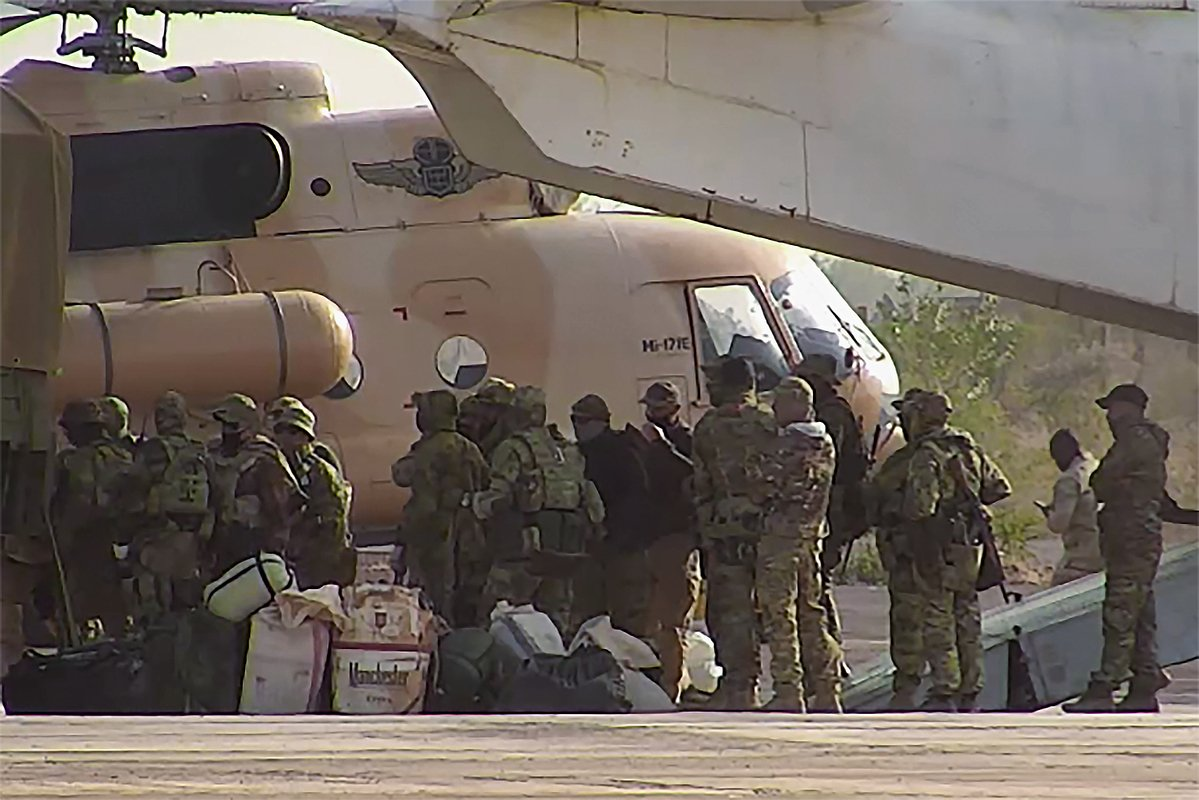
\includegraphics[width=0.75\textwidth]{img/pmc_africa_1.jpg}
    \caption{Предположительно сотрудники ЧВК «Вагнер» садятся в вертолет на севере Мали, фотография не датирована; Фото: French Army / AP}
\end{figure}

Также сообщалось, что за услугами «музыкантов» обращались различные политические силы в Ливии, Судане, Мозамбике, а также, возможно, власти Буркина-Фасо (хотя они это отрицают). По разным данным, в обмен структуры ЧВК «Вагнер», помимо финансового \ed{вознаграждения}{вознаграждение}{remuneration; compensation}, также получали доступ к добыче природных ресурсов в странах пребывания.

\begin{center}
    \Large

    Впрочем, министр иностранных дел России Сергей Лавров \ex{заверил}{reassured}, что никакой паники среди африканских коллег не заметил
\end{center}

Напротив, ряд африканских представителей связались с ним, чтобы выразить свою солидарность с российским руководством. По его словам, правительства Мали и ЦАР, помимо пригожинской ЧВК, поддерживают контакты с официальными властями, а несколько сотен военнослужащих, которые работают в ЦАР в качестве инструкторов, продолжат свою работу, несмотря на последние события.

При этом официальный представитель Министерства иностранных дел (МИД) России Мария Захарова уточнила, что решение о продолжении работы в Африке непосредственно специалистов ЧВК «Вагнер» будут принимать сами африканские страны. Также она подчеркнула необходимость отделять обычных бойцов от организаторов мятежа, призвав «смотреть не на trademark ``Вагнер'', не на термин, а на суть».

\begin{wrapfigure}{r}{0.5\textwidth}
    \begin{fancyquotes}
        Она заключается в том, что за последние годы люди это доказали, занимаясь на фронте, на передовой, обеспечением нашей безопасности (...) проявляли себя соответствующим образом в Сирии, в африканских государствах

        \begin{flushright}

            Мария Захарова\\

            пресс-секретарь МИД России
        \end{flushright}
    \end{fancyquotes}
\end{wrapfigure}
Однако непонятно, позволят ли бойцам оставаться в Африке под тем самым trademark «Вагнер». В своем обращении президент России Владимир Путин дал «музыкантам» выбор из трех вариантов: заключить контракт с Министерством обороны России или другим силовым органом, вернуться домой к родным или «уйти в Белоруссию».


\begin{center}
    \Large
    \ed{Затрагивают}{затрагивают}{affect} или нет эти слова и тех бойцов ЧВК «Вагнер», что находятся в Мали и ЦАР, непонятно
\end{center}


\begin{figure}[h]
    \centering
    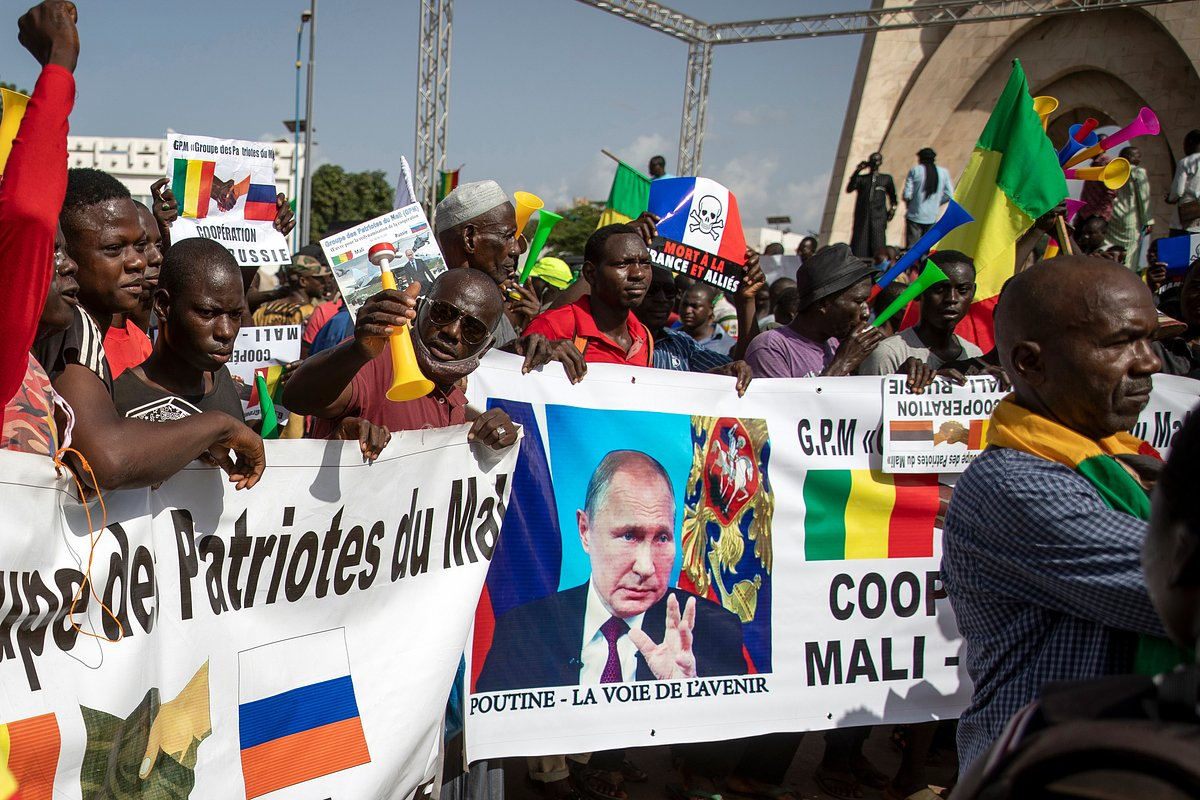
\includegraphics[width=0.75\textwidth]{img/pmc_africa_2.jpg}
    \caption{Жители Мали на демонстрации против Франции и в поддержку России по случаю 60-летия независимости страны, Бамако, 22 сентября 2020 года; Фото: AP }
\end{figure}

Более того, глава комитета Государственной Думы по обороне Андрей Картаполов заявил: отказавшиеся от подписания договоров формирования не будут получать «ни денег, ни финансовых, ни материальных ресурсов». Как отмечает The Financial Times, без материальной и логистической поддержки российских властей вагнеровцам будет крайне сложно продолжить работать в Африке.

\begin{center}
    {\Huge 86,3}\\
    {\huge млрд рублей}\\[1em]

    {\Large выплачено ЧВК «Вагнер» из госбюджета с мая 2022 года по май 2023 года }
\end{center}

«Лента.ру» направила запрос в пресс-службу Министерства обороны России с просьбой прояснить позицию ведомства по данному вопросу. На момент публикации материала ответа не поступило.

\begin{center}
    \Large Сам Евгений Пригожин не рассказывал, чем дальше будет заниматься его ЧВК «Вагнер» и сохранится ли ее африканское подразделение
\end{center}


\begin{figure}[h]
    \centering
    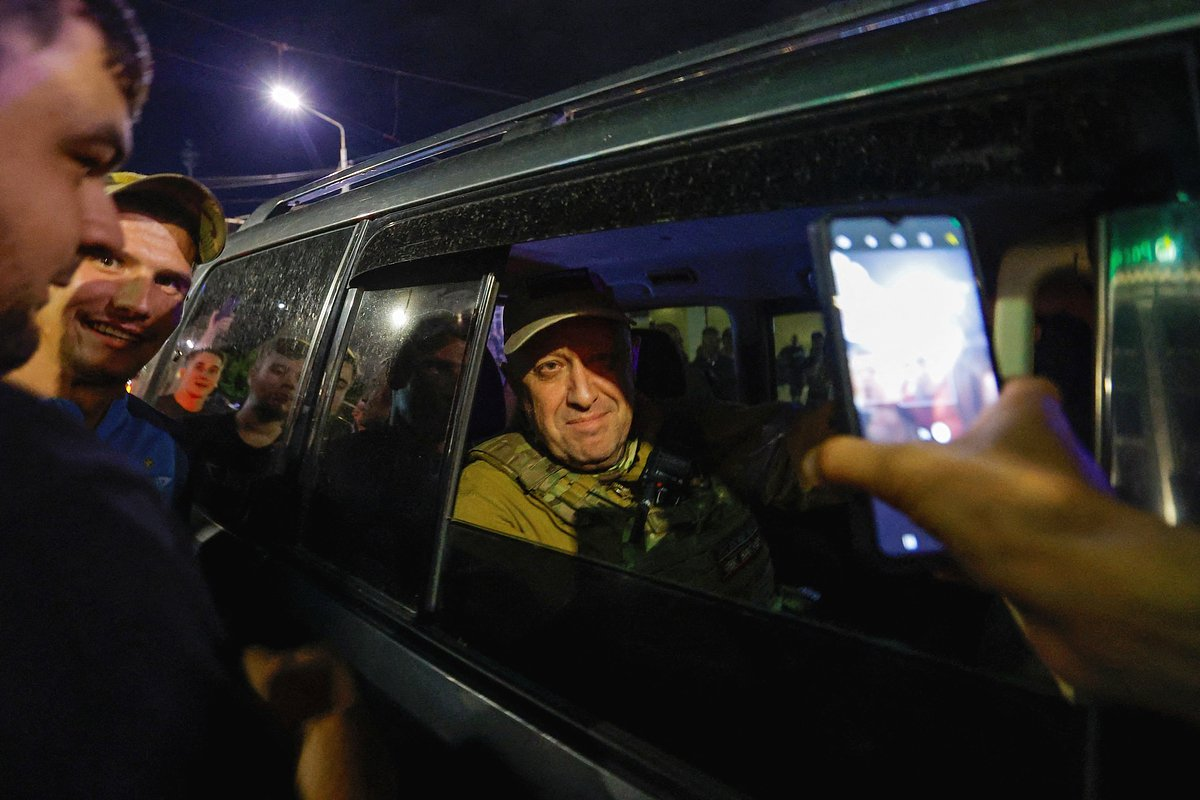
\includegraphics[width=0.75\textwidth]{img/pmc_africa_3.jpg}
    \caption{Евгений Пригожин покидает штаб Южного военного округа в Ростове-на-Дону, 24 июня 2023 года; Фото: Alexander Ermochenko / Reuters}
\end{figure}

Президент Белоруссии Александр Лукашенко, выступивший в качестве посредника между российскими властями и Евгением Пригожиным, заявил, что ушедшие в республику вагнеровцы могут быть привлечены к обучению местных подразделений.

Впрочем, пока дипломаты в ЦАР не заметили очевидных перемен в обстановке в стране после мятежа: представители ЧВК «Вагнер» были замечены в Банги и после событий 24 июня, сообщает The Financial Times. При этом местные власти уже выразили готовность принять от России любую военную помощь.

\begin{fancyquotes}
    Если Москва решит отозвать вагнеровцев и прислать вместо них «бетховенов» или «моцартов», мы будем не против

    \begin{flushright}
        Фидель Гуанджики\\
        советник президента ЦАР
    \end{flushright}
\end{fancyquotes}

The Financial Times отмечает, что речь может идти про другие российские ЧВК, \ex{предположительно}{presumably} связанные с «Газпромом».

Необходимо учитывать, что многие проекты ЧВК «Вагнер» в Африке были \ed{убыточными}{убыточный}{unprofitable} и \ed{дотационными}{дотационный}{subsidized}, то есть часть расходов на них прямо или \ex{к\'{о}свенно}{indirectly} компенсировалась из бюджета, отмечает директор Центра изучения Африки НИУ ВШЭ Андрей Маслов. По его словам, те проекты, где доходная база генерируется в самой Африке, могут претерпеть ребрендинг, тогда как дотационные проекты могут быть переданы под контроль Министерства обороны России и продолжить реализовываться в формате официальной поддержки по развитию местных вооруженных сил.

\begin{wrapfigure}{l}{0.5\textwidth}
    \begin{fancyquotes}
        Как показывает практика, такой формат более эффективен и несет в себе меньше рисков. Прямое сотрудничество имеет большие перспективы и более стабильно

        \begin{flushright}
            Андрей Маслов\\
            директор Центра изучения Африки НИУ ВШЭ
        \end{flushright}
    \end{fancyquotes}
\end{wrapfigure}
Африканист также призвал не \ex{переоценивать}{overestimate} роль ЧВК «Вагнер» --- и в архитектуре российско-африканских связей, и в архитектуре связей в области обороны и безопасности в регионе. Он напомнил, что Россия заключила официальные соглашения с десятками африканских государств, а в ЦАР по согласованию с ООН работают российские инструкторы от Министерства обороны России.

При этом масштаб деятельности ЧВК «Вагнер» в Африке сильно преувеличен как самой структурой и связанной с ней сеткой Telegram-каналов, так и западными чиновниками, которые запугивают африканцев и самих себя «ужасными русскими наемниками», полагает эксперт. Более того, ни Мали, ни ЦАР не входят в десятку ведущих африканских партнеров России по объемам торговли и инвестиций.

\begin{center}
    \Large
    Андрей Маслов предположил, что сотрудничество с Мали и ЦАР продолжится по линии Министерства обороны России — произойдет своего рода «национализация» программ содействия местным вооруженным силам
\end{center}

\begin{figure}[h]
    \centering
    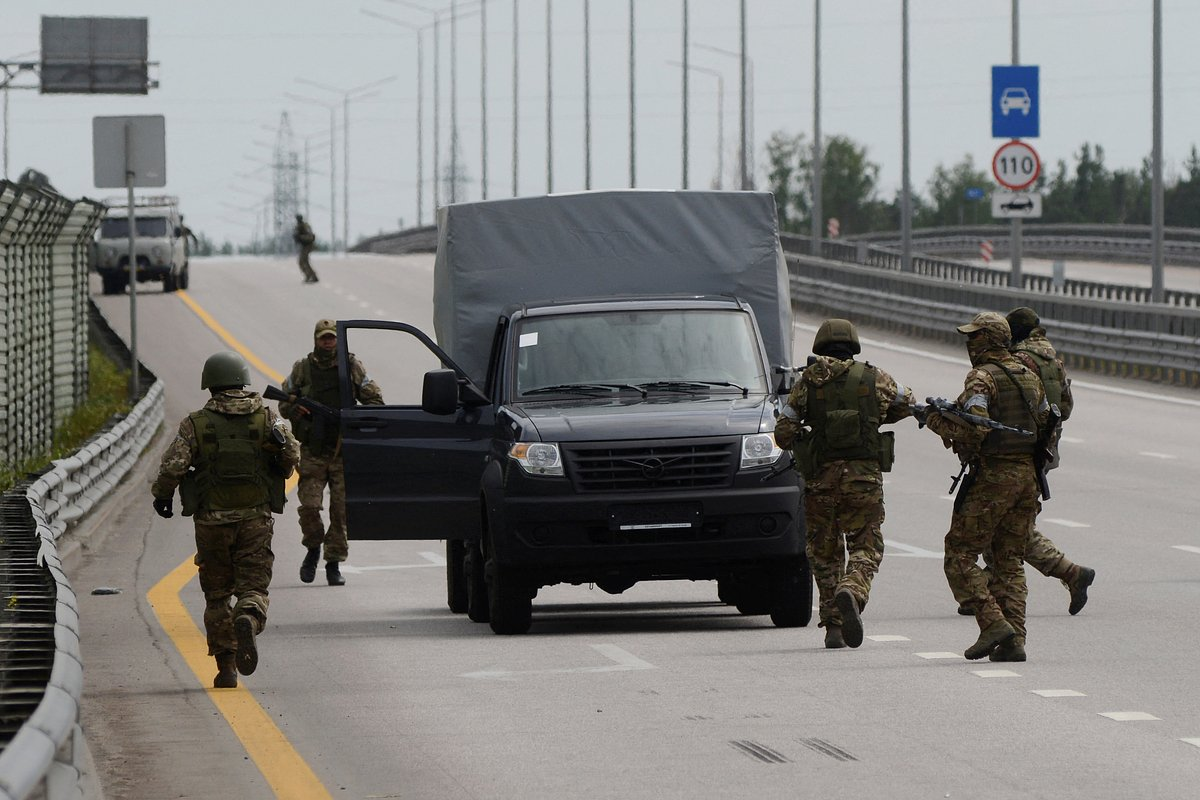
\includegraphics[width=0.75\textwidth]{img/pmc_africa_4.jpg}
    \caption{Бойцы ЧВК «Вагнер» обходят автомобиль на трассе М-4 недалеко от Воронежа, 24 июня 2023 года; Фото: Reuters}
\end{figure}

Что касается Мали, то Россия может быть заинтересована, например, в усилении роли Алжира в вопросах обеспечения безопасности в Сахаре, поскольку это североафриканское государство обладает значительным опытом в данной сфере и остается верным и крепким союзником России. Разумеется, сотрудничество с Алжиром никоим образом не должно идти в ущерб суверенитету Мали.

% -- <> -- 
\begin{fancyquotes}
    Поэтому российская сторона заинтересована в укреплении межгосударственных связей на региональном уровне и усилении африканского компонента в обеспечении безопасности. В долгосрочной перспективе это даст нам преимущества

    \begin{flushright}
        Андрей Маслов\\
        директор Центра изучения Африки НИУ ВШЭ
    \end{flushright}

\end{fancyquotes}

\textbf{Китайские стражи.} На африканском континенте, помимо ЧВК «Вагнер», работает множество частных военных компаний: американские CACI и Constellis, британские Aegis Defence Services и G4S, французская Secopex, немецкая Asgaard и многие другие.

\begin{center}
    \Large
    Специалисты затрудняются назвать даже примерное число иностранных наемников в Африке
\end{center}

Дело в том, что местные политические силы не любят афишировать свои связи с подобными структурами, а сами компании, как правило, заключают соглашения о неразглашении, запрещающие им делиться подробной информацией о характере их работы в африканских странах.

Впрочем, Андрей Маслов усомнился, что западные военные компании могут создать альтернативу ЧВК «Вагнер», поскольку изначально занимают другую нишу, работая с корпоративным сектором и занимаясь охраной объектов западных добывающих компаний. Африканские государства-заказчики же при выборе подрядчиков исходят из своих внешнеполитических приоритетов, а не из рыночных условий: что Мали, что ЦАР воспринимали ЧВК «Вагнер» как рекомендованную российским государством структуру.

\begin{fancyquotes}
    Какой частной она бы ни была, для Мали и ЦАР важно то, что она российская. Поэтому вряд ли произойдет вытеснение ЧВК «Вагнер» иностранными структурами на рыночных условиях


    \begin{flushright}
        Андрей Маслов\\
        директор Центра изучения Африки НИУ ВШЭ
    \end{flushright}

\end{fancyquotes}


\begin{figure}[h]
    \centering
    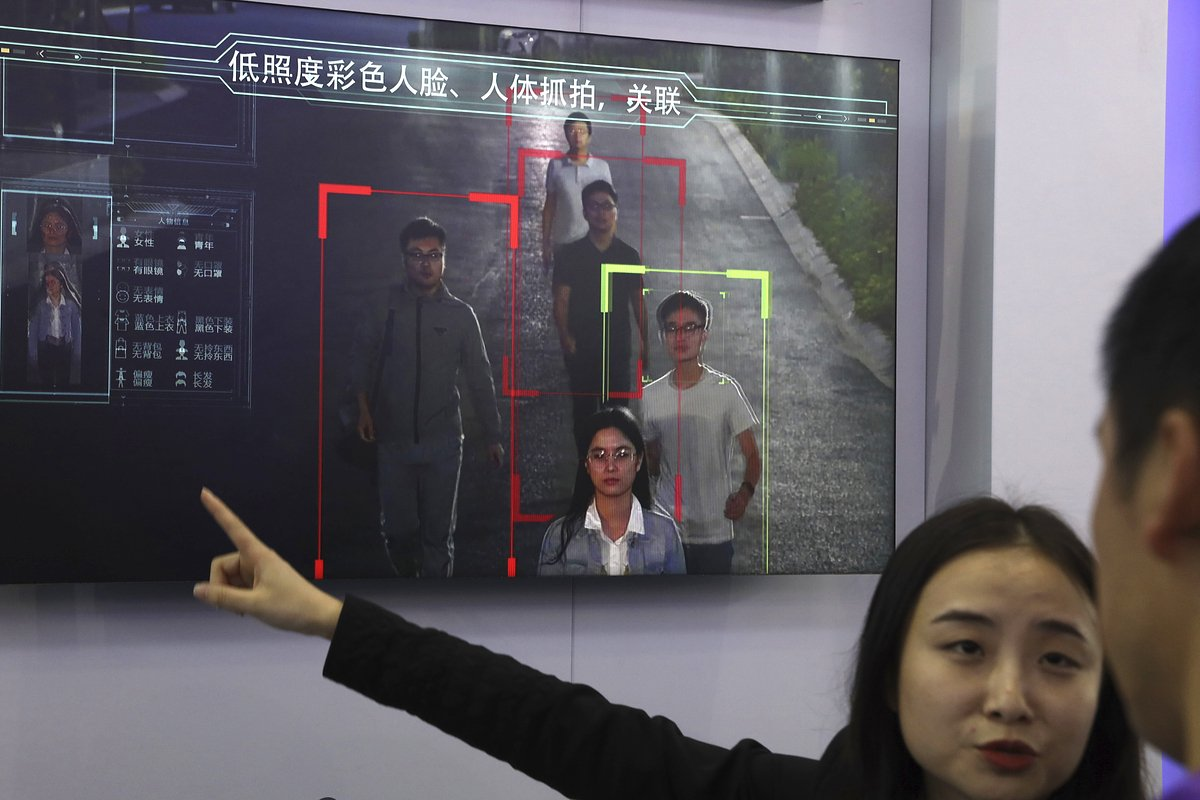
\includegraphics[width=0.75\textwidth]{img/pmc_africa_5.jpg}
    \caption{Презентация технологии идентификации человека от государственного производителя оборудования для наблюдения Hikvision на выставке Security China 2018 в Пекине, Китай, 23 октября 2018 года; Фото: Ng Han Guan / AP}
\end{figure}

Особняком стоят частные охранные фирмы из Китая, начавшего масштабную экономическую экспансию на континент в рамках запущенной в 2013 году инициативы «Один пояс — один путь»: соответствующие соглашения подписаны с 52 из 54 африканских стран. К настоящему моменту в Африке работает около 10 тысяч китайских компаний и, по разным оценкам, от 1 до 2 миллионов китайских рабочих, задействованных в развитии инфраструктуры, строительстве жилья, промышленном производстве и добыче полезных ископаемых.

Однако обстановка с безопасностью в ряде африканских стран оставляет желать лучшего: на континенте орудуют многочисленные вооруженные группировки, для которых похищение иностранных рабочих — один из основных источников дохода. Рабочих из Китая считают лакомой добычей: китайские корпорации, как правило, не жалеют денег, чтобы вызволить своих сотрудников.

\begin{center}
    \Large
    Полагаться на местные органы безопасности не приходится, тем более с учетом довольно неспокойной внутриполитической обстановки в ряде стран Африки: китайские рабочие не раз оказывались буквально меж двух огней враждующих фракций
\end{center}

Все это подтолкнуло китайскую сторону к тому, чтобы самостоятельно заняться защитой своих граждан, благо есть кем: в Поднебесной зарегистрировано свыше пяти тысяч частных охранных компаний, в которых работает около четырех миллионов человек, преимущественно из числа бывших военных.

\begin{center}
    \Large
    Частные военные компании в Китае запрещены, а все охранные предприятия строго подконтрольны Министерству общественной безопасности КНР
\end{center}

За пределами Китая разрешено работать всего 20 компаниям, а в Африке работает по меньшей мере девять из них: Beijing DeWe Security Service, Hua Xin Zhong An Group, Shandong Huawei Security Group, China Security Technology Group, China Overseas Security Group, Frontier Services Group, China Overseas Security Service, VSS Security Group и Zhongjun Junhong Security Service.


\begin{figure}[h]
    \centering
    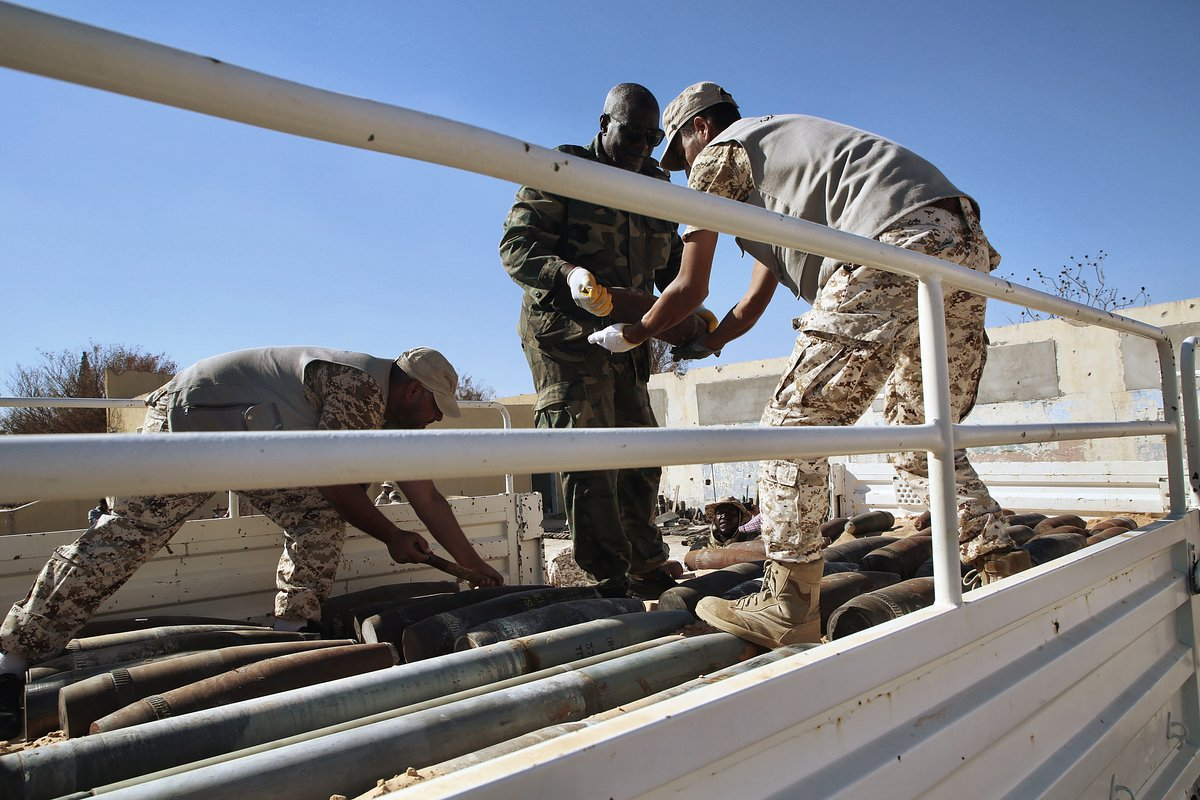
\includegraphics[width=0.75\textwidth]{img/pmc_africa_6.jpg}
    \caption{Ливийские ополченцы и специалсты из ЧВК «Вагнер» на погрузке боеприпасов, район Аль-Хира, в 75 километрах к югу от Триполи, Ливия, 22 июля 2020 года; Фото: Hazem Turkia / Anadolu Agency / Getty Images}
\end{figure}

По официальным данным, за границей работают всего 3200 сотрудников китайских частных охранных фирм, но исследователи полагают, что цифры сильно занижены: в одной лишь Кении защитой строительства железной дороги Момбаса — Найроби — Найваша занималось 2000 сотрудников DeWe.

Василий Кашин, директор Центра комплексных европейских и международных исследований НИУ ВШЭ и специалист по китайскому военно-промышленному комплексу, отмечает, что подавляющему большинству подобных фирм запрещено пользоваться оружием. Исключение составляют сотрудники Overseas Security Guardians и Hua Xin Zhong An Group, которые обеспечивают вооруженный конвой для китайских судов, следующих в африканских водах.

В остальных случаях сотрудники подобных фирм организуют охрану китайских предприятий с помощью нелетальных вооружений, решают технические задачи и выстраивают партнерство с местными охранными структурами. «А задачи, требующие использования оружия, они решают как раз за счет найма местных партнеров», — рассказал Василий Кашин в беседе с «Лентой.ру».

Например, в июле 2016 года DeWe прибегла к найму местных вооруженных сотрудников, чтобы эвакуировать свыше 300 китайских нефтяников из южно-суданской столицы Джубы, в которой разгорелось вооруженное противостояние между правительственными и оппозиционными силами.

Таким образом, китайские охранные предприятия значительно отличаются от структур ЧВК «Вагнер» — и по своему устройству, и по своим задачам, а потому вряд ли станут альтернативой российской компании в случае ее ухода с континента, считает специалист.

\begin{fancyquotes}
    Китайцам страшно помыслить о том, чтобы разрешить своему охранному бизнесу заниматься тем же, чем занимался «Вагнер»

    \begin{flushright}
        Василий Кашин\\
        директор Центра комплексных европейских и международных исследований НИУ ВШЭ
    \end{flushright}
\end{fancyquotes}

\textbf{Новые башибузуки.} Еще один игрок на африканском континенте, который может воспользоваться уходом вагнеровцев, — турецкая частная военная компания Sadat International Defense Consultancy, основанная в 2012 году. На официальном сайте утверждается, что SADAT — это «первая и единственная частная ЧВК в Турции, которая на международном уровне предоставляет услуги консалтинга, военной подготовки и логистики в секторе международной обороны и внутренней безопасности».

\begin{center}
    \Large
    Одним из главных преимуществ турецкой ЧВК SADAT считается наличие «готовых военно-воздушных сил», вооруженных беспилотниками Bayraktar, зарекомендовавшими себя в конфликтах на Украине, в Нагорном Карабахе и Ливии
\end{center}

\begin{figure}[h]
    \centering
    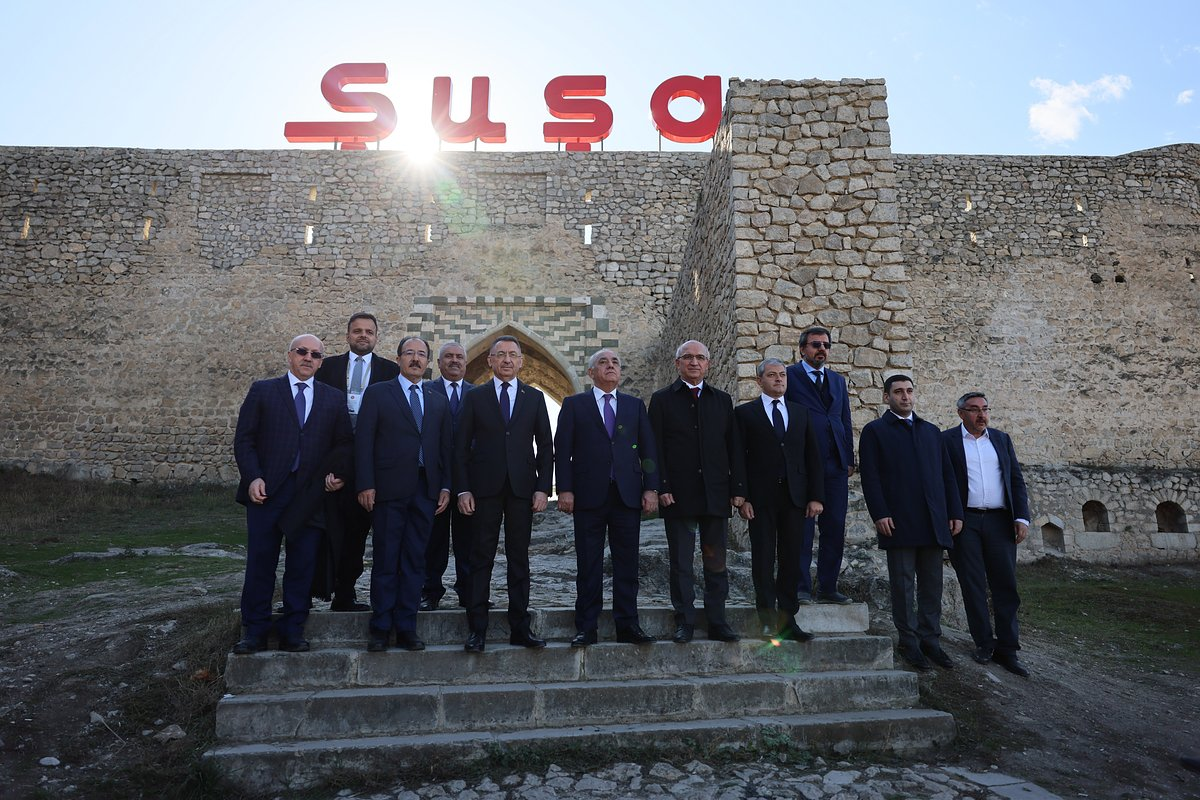
\includegraphics[width=0.75\textwidth]{img/pmc_africa_7.jpg}
    \caption{Вице-президент Турции Фуат Октай и премьер-министр Азербайджана Али Асадов посещают город Шуша в Нагорном Карабахе, Азербайджан, 5 ноября 2022 года; Фото: Berke Bayur / Anadolu Agency / Getty Images}
\end{figure}


Ряд наблюдателей считает SADAT личной армией президента Турции Реджепа Тайипа Эрдогана. Во время попытки госпереворота в июле 2016 года бойцы SADAT участвовали в подавлении протестов и, вероятно, даже стреляли по гражданским, рассказывает старший научный сотрудник American Enterprise Institute Майкл Рубин. С 2016 по 2022 год основатель SADAT Аднан Танрыверди также занимал пост главного военного советника турецкого лидера. При этом сам Реджеп Эрдоган опровергает всякие обвинения в покровительстве ЧВК.

По различным данным, SADAT работает в Сомали и Катаре, сотрудничала с палестинским движением ХАМАС и обучала ливийских повстанцев и сирийских боевиков, выступавших против правительства Башара Асада, в том числе якобы завербованных на Кавказе бойцов «Исламского государства» и «Джебхат ан-Нусры» (террористическая группировка, запрещенная в России).

ЧВК, вероятно, также была активно задействована и в конфликте в Нагорном Карабахе осенью 2020 года. По сведениям газеты «Коммерсант», SADAT занималась вербовкой и подготовкой сирийских боевиков на подконтрольных Турции территориях на севере и северо-западе Сирии, после чего обученных наемников — около 1,3 тысячи бойцов — перебросили в зону конфликта на чартерах, зафрахтованных все той же SADAT.

Кроме того, осенью 2022 года сообщалось о планах ЧВК направить своих наемников в Кашмир, являющийся предметом территориального спора между Индией и Пакистаном.

\begin{center}
    \Large
    В самом SADAT настаивают, что не участвуют в конфликтах в качестве наемников, а оказывают исключительно консультационные и образовательные услуги
\end{center}


\begin{figure}[h]
    \centering
    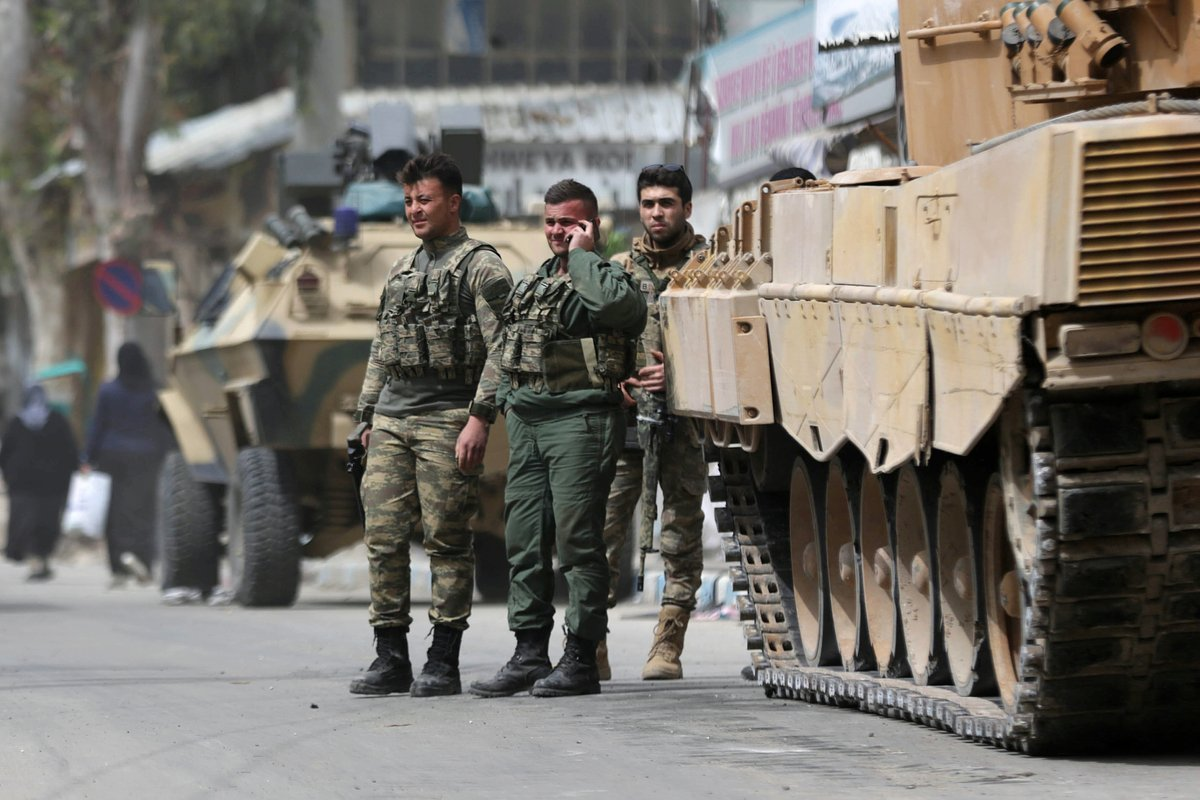
\includegraphics[width=0.75\textwidth]{img/pmc_africa_8.jpg}
    \caption{Турецкие солдаты в центре Африна, Сирия, 24 марта 2018 года; Фото: Khalil Ashawi / Reuters}
\end{figure}

Как и многие другие страны, в последние годы Турция активно развивает официальные связи с Африкой: страна значительно расширила свою сеть посольств на континенте, а ее президент посетил больше африканских государств, чем кто-либо из неафриканских лидеров.

Особое внимание уделяется наращиванию военно-технического сотрудничества с Африкой: лишь за 2021 год поставки турецкого военного оборудования на континент выросли в пять раз, правда, занимают пока меньше одного процента от рынка. Впрочем, этот показатель, вероятнее всего, продолжит расти — не в последнюю очередь благодаря растущей популярности турецких дронов Bayraktar.

Помимо Ливии, турецкие военные присутствуют в Сомали, где обучают местных солдат и офицеров военному ремеслу, причем на турецком языке, а сомалийские новобранцы даже приносят присягу сразу на двух языках. Кроме того, турецкие военнослужащие задействованы в миротворческих миссиях ООН в Демократической Республике Конго, Мали, Сомали, Судане, Южном Судане и ЦАР.

Впрочем, основатель SADAT Аднан Танрыверди еще в 2019 году призвал к переменам: по его словам, Турции необходимо создать полноценный аналог американской Blackwater, бойцы которой отправятся выполнять военные задачи в Африку, тогда как официальные вооруженные силы сосредоточатся на обороне собственной страны.

\begin{fancyquotes}
    Турция имеет глубоко укоренившиеся военные традиции. ЧВК могут оказывать услуги дружественным странам, нанимая отставных и недавно демобилизованных солдат. А затем их можно будет использовать как инструмент внешней политики

    \begin{flushright}
        Аднан Танриверди\\
        основатель SADAT
    \end{flushright}
\end{fancyquotes}

Впрочем, чтобы отказаться от услуг россиян в пользу турков, африканские государства, где сейчас работает ЧВК «Вагнер», должны будут сначала изменить свой политический курс, отмечает Андрей Маслов.

\begin{fancyquotes}
    Но пока предпосылок к тому, чтобы ЦАР или Мали поменяли свой внешнеполитический вектор, мы не видим

    \begin{flushright}
        Андрей Маслов\\
        директор Центра изучения Африки НИУ ВШЭ
    \end{flushright}
\end{fancyquotes}

Сам основатель SADAT Аднан Танрыверди другим важным условием считает разработку турецкими властями законодательства, которое бы устанавливало контроль государства над будущими военными компаниями. Мятеж Евгения Пригожина, вероятно, может ускорить этот процесс. Впрочем, все те же события 24 июня могут заставить Реджепа Эрдогана, наоборот, более настороженно отнестись к легализации и расширению сферы деятельности ЧВК — тем более что в 2016 году он уже пережил одну попытку госпереворота.

Китайские и турецкие ЧВК вряд ли сумеют составить достойную альтернативу ЧВК «Вагнер» в обозримом будущем: и в силу их текущей структуры и сфер деятельности, и в силу того, что сами Китай с Турцией, по всей видимости, не особо к этому стремятся. Западные ЧВК тоже не смогут претендовать на нишу вагнеровцев — их клиенты в основной своей массе крайне негативно относятся к перспективе сотрудничества с «неоколониальными силами» и изначально обратились к россиянам именно из этих соображений.

\begin{center}
    \Large
    Наконец, не похоже на то, что Россия сама готова отказаться от целого измерения сотрудничества со странами континента
\end{center}

Вероятно, российские власти выработают какое-то решение, которое позволит специалистам ЧВК «Вагнер» и дальше оказывать свои услуги в странах Африки в обмен на определенные гарантии лояльности. А уж под каким брендом — особой роли не играет: в африканских странах дали четко понять, что будут рады любым российским «музыкантам» — хоть «бетховенам», хоть «моцартам».

\newpage
\section{Караганов призвал Кремль нанести ядерный удар по Польше}

\textit{Спецкор «Медузы» Андрей Перцев объясняет, почему эти угрозы на самом деле опаснее, чем оголтелые посты Дмитрия Медведева}

\textit{Источник: \url{https://meduza.io}}
% https://meduza.io/feature/2023/06/15/politolog-sergey-karaganov-prizval-kreml-nanesti-yadernyy-udar-po-polshe

\textit{Журнал «Профиль» опубликовал — а издание «Россия в глобальной политике» перепечатало — статью политолога Сергея Караганова, суть которой сводится к тому, что Россия «должна нанести превентивный ядерный удар по Европе», чтобы «сломить волю Запада» и \explain{добиться победы}{achieve victory; добиться + чего} в войне с Украиной. Угрозы применения ядерного оружия со стороны Москвы звучат буквально с первых недель полномасштабной агрессии (этим занимается и сам Путин). Тем не менее статья Караганова, к сожалению, выглядит не просто очередным сотрясанием воздуха. \ed{Спецкор}{спецкор}{специальный корреспондент} «Медузы» Андрей Перцев объясняет почему.
}

\textbf{Кто такой Сергей Караганов? И почему его статья вообще \explain{заслуживает внимания}{deserved attention}?}

Доктора исторических наук и политолога Сергея Караганова вы, возможно, помните по проекту «\ed{Намедни}{нам\'{е}дни}{на днях; недавно}. Наша эра» журналиста Леонида Парфенова. Он комментировал советскую политическую историю — и делал это во вполне либеральном ключе. Еще в 2011 году Караганов, например, проповедовал «декоммунизацию» и «десталинизацию».

С тех пор многое поменялось. Сейчас Сергей Караганов --- один из основателей российского Совета по внешней и оборонной политике (СВОП). Это экспертный центр, с которым сотрудничают бывшие военные, дипломаты, действующие политики, исследователи и журналисты. В 2004 году СВОП стал одним из учредителей клуба «Валдай», в заседаниях которого регулярно участвует Путин. Сам Караганов, разумеется, тоже посещает эти встречи. Заседания клуба модерирует его соратник по СВОП, журналист-международник и политолог Федор Лукьянов. Он же возглавляет журнал «Россия в глобальной политике», а Караганов руководит редакционным советом издания.

\begin{wrapfigure}{l}{0.45\textwidth}
    \centering
    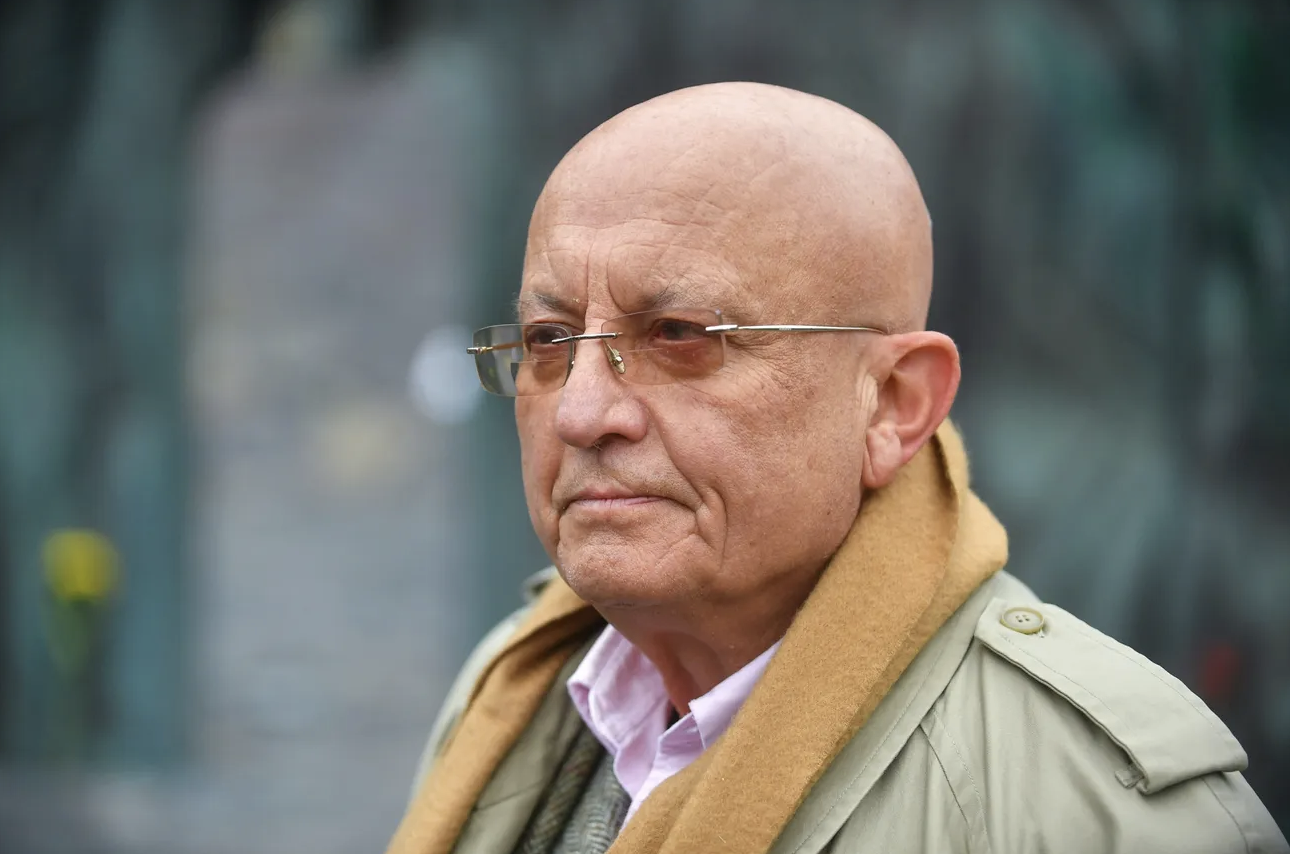
\includegraphics[width=0.43\textwidth]{img/karaganov.png}
    \caption{Сергей Киселев / Агентство «Москва»}
\end{wrapfigure}
У Караганова есть еще одна высокая регалия --- научный руководитель факультета мировой экономики и мировой политики Высшей школы экономики. Но самое главное, что он входит в состав научного совета при Совете безопасности РФ, который на фоне вторжения стал, по всей видимости, ключевым органом власти в России. Два источника «Медузы», близких к администрации президента (АП), называют Караганова человеком, который «может влиять на мнение секретаря Совбеза Николая Патрушева». А тот, в свою очередь, как считается, входит в близкий круг Путина.

Впрочем, третий собеседник «Медузы», близкий к Кремлю, призывает «не преувеличивать влияние Караганова». Тем не менее политолог реально участвует в деятельности Совета безопасности РФ и регулярно бывает на мероприятиях с участием Путина.

По косвенным признакам можно предположить, что руководители силового блока как минимум знакомы с идеями Караганова, а может быть, даже \explain{вдохновляются}{are inspired} ими. Вы наверняка слышали эксцентричные высказывания Николая Патрушева и главы Службы внешней разведки Сергея Нарышкина о том, что Польша «готовится захватить украинские земли» (подробнее об этом читайте, например, \href{https://carnegieendowment.org/politika/88530}{тут}). Так вот: Караганов \href{https://globalaffairs.ru/articles/rakety-v-evrope-vospominaniya-o-budushhem/}{рассуждал} об этом еще в 2016 году:

\begin{fancyquotes}
    Она (Украина) вряд ли может состояться как государство в долгосрочной перспективе. Скорее всего, страна будет медленно распадаться. Ну а там история покажет. Не исключено, что что-то может отойти к России, что-то — к Венгрии, что-то — к Польше, а что-то может остаться формально независимым Украинским государством.
\end{fancyquotes}

\textbf{Дмитрий Киселев в прямом эфире грозил превратить США в «радиоактивный пепел» еще до аннексии Крыма. А недавно ядерным ударом пугал Запад Дмитрий Медведев. Неужели слова политолога Караганова значат больше?}

В каком-то смысле да. Дмитрий Киселев в середине 2010-х был главным пропагандистом российской власти. В этом качестве он театрально и, \explain{по всей видимости}{apparently}, совершенно \explain{осознанно}{consciously} \explain{эпатировал}{shocked, scandalised} либерально настроенных \ed{сограждан}{согражданин}{fellow citizen} --- выступая с речами, вызывающими ужас и стыд, но не имеющими никаких последствий. Примерно тем же (несмотря на свой прежний и нынешний\footnote{Формально бывший президент и бывший премьер Медведев остается заместителем Путина в Совбезе РФ. Эту должность придумали специально для него, чем он там занимается, неизвестно.} высокий статус) занимается и Медведев, который в своем телеграм-канале оскорбляет западных политиков и жителей других стран.

В случае Киселева и Медведева угрозы ядерным оружием воспринимаются в ряду других не менее жестких заявлений. В отличие от Киселева и Медведева, Караганов всегда вел себя сдержанно. При этом его статья перепечатана в журнале «Россия в глобальной политике»: это медиа когда-то было запущено по модели западного аналитического издания при участии американского журнала Foreign Affairs — и до последнего времени считалось серьезным и уважаемым. Даже после 24 февраля журнал не исключили из международных баз данных научных публикаций (например, Scopus), то есть публиковаться там, в том числе зарубежным ученым, по-прежнему допустимо и даже — теоретически — престижно.

Статью Караганова, вероятно, можно воспринять как личную инициативу, попытку послать сигнал высшему руководству страны — и предложить свой радикальный вариант выхода из кризиса, в котором Россия оказалась из-за военной агрессии против Украины. С другой стороны, учитывая близость Караганова к Совбезу РФ и его личное участие в организации «Валдая», этот текст вполне может транслировать мнение, распространенное в силовом — самом влиятельном — блоке российской власти.

\textbf{То есть это статья написана лично для Путина?}

Возможно. \ed{В пользу}{в пользу}{in favour} этой версии говорит риторика, которую использует Сергей Караганов. Она очень близка российскому президенту: политолог явно пытается соответствовать путинскому языку. Например, в тексте встречается «пацанская аргументация», характерная для президента РФ: в частности, когда Караганов объясняет, что превентивный ядерный удар по Европе нужен, «чтобы Запад просто ``отвалил'' и не мешал\footnote{мешать + кому} России и миру идти вперед». Не забыл Караганов упомянуть и «неоколониализм», который в последние полтора года \explain{к месту}{in place} и не к месту вспоминает Путин.

Или вот еще одно, по сути, повторение излюбленных путинских клише:

\begin{fancyquotes}
    Запад теряет имевшуюся у него на протяжении пяти веков возможность \ex{высасывать}{suck} богатство из всего мира, \ed{навязывая}{навязывать}{to impose}, в первую очередь грубой силой, политические, экономические порядки и устанавливая свое культурное доминирование. Так что быстрого окончания развертываемой Западом оборонительной, но агрессивной конфронтации ожидать не приходится.
\end{fancyquotes}

Караганов вспоминает также «отрицание семьи, родины, истории, любви между мужчиной и женщиной, веры, служения высшим идеалам, всего того, что составляет сущность человека» --- все это, разумеется, на Западе. Узнаете? Да, Путин тоже об этом много и часто говорит.

При этом автор успокаивает своего потенциального высокопоставленного читателя --- того самого, который гипотетически может принять решение о применении ядерного оружия: США якобы не \ed{вст\'{у}пятся за}{вступ\'{и}ться за кого-либо}{to stand up for} Европу, никто не будет жертвовать «условным Бостоном ради условной Познани». Караганов \ex{подкрепляет}{reinforces} эту мысль еще одним опасным тезисом: «Победителей не судят, а спасителей благодарят». А что победа в итоге окажется за Россией, как бы само собой разумеется.

Насколько лет назад Караганов доказывал, что ядерное оружие, которым располагает Россия, было залогом отказа Запада от поставок оружия Украине во время войны в Донбассе 2014–2015 годов:

\begin{fancyquotes}
    Когда горячие головы в Вашингтоне требовали поставки Киеву «летальных вооружений», европейцы, да и руководство США категорически это \ex{отвергли}{rejected}, поскольку понимали, что Россия, прикрытая ядерным оружием и обретшая волю к борьбе, ответит крайне жестко.
\end{fancyquotes}

Но теперь, когда США и страны Евросоюза такое вооружение поставляют, получается, что Россия просто «обязана» сделать следующий опаснейший шаг.

Если Караганов (один или вместе с влиятельными единомышленниками) действительно хочет убедить президента РФ в необходимости нанести ядерный удар, вполне логично, что он доносит эту мысль в приятной и знакомой Путину обертке.

\textbf{Довольно пугающая версия. А другие есть?}

Да. Возможно, Караганов пытается не убедить Путина ударить по Европе, а напугать влиятельных и высокопоставленных людей на Западе самой этой возможностью --- и склонить их к изменению позиции по Украине.

Здесь нужно еще раз вспомнить об эволюции взглядов политолога. Даже после аннексии Крыма их еще можно было назвать относительно миролюбивыми. В 2016 году Караганов предлагал российским властям такую программу:

\begin{fancyquotes}
    Лучше бороться за мир, \ex{выступать поставщиком безопасности}{act as a security provider}, в том числе предотвращая дальнейшую экспансию западных союзов, что мы, хотя и \ex{с запозданием}{belatedly}, сделали в 2014 г. [аннексировав Крым], срывать планы тех, кто хочет вернуть гонку вооружений и системный военно-политический конфликт, восстановить лидерство в борьбе за верховенство международного права, за стратегическую стабильность.
\end{fancyquotes}

Тогда политолог был уверен, что «планов по завоеванию Украины у нас точно нет». Однако уже в 2017 году Караганов начал фокусировать внимание на том, что «одной из основ формирования нового миропорядка» может стать диалог США, России и Китая по вопросу о ядерном сдерживании. Иными словами, он стремительно разуверился в идее борьбы за мир и «верховенстве международного права» и пришел к выводу, что ядерное оружие — более надежный гарант мира на планете, чем договоренности и принципы:

\begin{fancyquotes}
    «Большая тройка» будет закладывать основы для менее хаотичной и более безопасной мировой системы будущего. Этот новый «концерт наций», если и когда у лидеров трех стран хватит чувства ответственности создать его, может оказаться более устойчивым, чем предыдущий из XIX века, если он по согласию будет базироваться на взаимном ядерном сдерживании, а не только на моральных принципах или балансе сил.
\end{fancyquotes}

То есть уже как минимум шесть лет Караганов уверен, что только страх перед использованием ядерного оружия может удержать человечество от кровопролитной глобальной войны, — и пытается убедить в этом своих читателей.

Нынешняя статья продолжает эволюцию взглядов политолога. Если в 2017 году Караганов еще предлагал сторонам спокойно подумать о переговорах, то теперь он пытается посеять у читателей на Западе страх и заставить их согласиться на уступки.

Караганов, очевидно, надеется, что в западных странах заметят: теперь им угрожает не потерявший влияние бывший президент (выбравший в качестве публичной стратегии оскорбления в адрес всего, чем раньше сам восхищался) и не штатный пропагандист в популярном вечернем шоу (которому полагается выступать с самыми радикальными идеями). К ним со страниц авторитетного — как, очевидно, полагают в редакции — журнала обращается серьезный эксперт, который не так уж давно считал ядерный конфликт маловероятным.

Вероятно, с точки зрения Караганова, это должно послужить лишним аргументом, чтобы Запад наконец отказался от поддержки Украины. В статье такой вариант прямо проговаривается: «Все-таки велика вероятность, что удастся победить, образумить противника без крайних мер, заставить его отступить».

Иными словами, сам Караганов может считать свой текст дополнительным элементом «ядерного сдерживания».

\textbf{Но если статья Караганова — не более чем его личное послание (хоть Путину, хоть Западу), то бояться все равно нечего?}

К сожалению, даже в этом случае появление такой статьи — плохая новость. Во-первых, не будем забывать, что у автора могут быть влиятельные единомышленники. Во-вторых, слишком логичными и убедительными могут казаться Путину и его окружению рассуждения Караганова о ходе исторического процесса: Запад «умирает и теряет влияние»; его нужно огорошить мощным ударом; история будет «на нашей стороне».

Даже если цель Караганова только в том, чтобы напугать Запад, его статья вполне способна повлиять на решения руководства России. Из-за стремления звучать в унисон с Путиным текст может оказаться не элементом ядерного сдерживания, как, возможно, надеялся сам автор, а ступенькой вверх по лестнице ядерной эскалации.

Правда, аналитик британского исследовательского центра Chatham Housе Кеир Джайлс предлагает относиться к ядерным угрозам, звучащим из России, исключительно как к методу психологической войны. Как отмечает Джайлс, Кремль прибегает к этому методу всякий раз, когда у российской армии возникают реальные проблемы на фронте (а статья Караганова появилась вскоре после начала украинского контрнаступления). Но и Джайлс признает: Путин действительно ориентируется на пропагандистские СМИ и лояльных экспертов, и это может роковым образом влиять на решения президента РФ.

Вот понятный пример. Перед полномасштабным вторжением в Украину верхушка ФСБ убеждала Путина, что украинцы с цветами встретят российских солдат. Причем не факт, что все «ястребы» сами хотели большой войны — скорее, стремились угодить главе государства. Но в итоге, оперевшись на эти высказывания и оценки, Путин начал реальную агрессию.

Теперь игра, затеянная Карагановым с не самыми ясными намерениями, вполне может показаться руководству России планом легкой победы.


\clearpage

% \chapter{История}

\section{Море долго выбрасывало тр\'{у}пы**}

\textit{70 лет назад цунами разрушило советский город. Как власти скрывали смерть тысяч человек?}

\textit{Источник: \url{https://lenta.ru/articles/2022/11/05/tsunami1952/}}

Р\'{о}вно 70 лет назад, 5 ноября 1952 года, мощное цунами разрушило город Северо-Курильск на острове Парамушир в Сахалинской области, и смыло несколько соседних \ed{посёлков}{посёлок}{settlement}. Точное число погибших до сих пор неизвестно. По официальной версии, в одном только Северо-Курильске пог\'{и}бло 1200 человек из 6000 населения, а \explain{с учётом}{taking into account} соседних населённых пунктов эта цифра превышает 2000 человек. Историки говорят, что погибших могло быть \explain{в раз\'{ы} больше}{many times more}. Трагедию засекр\'{е}тили: п\'{е}рвые данные о ней опубликовали только в начале 1990-х, но некоторые военные архивы недоступны до сих пор. Как произошла самая масштабная забытая катастрофа СССР и как её пытались забыть --- в материале «Ленты.ру».

\textbf{«Накануне вся природа затихла»}

Ночью 5 ноября 1952 года в Тихом океане случилось мощное землетрясение магнитудой 8,3 по шкал\'{е} Рихтера. Его эпицентр находился приблизительно в 200 километрах от Петропавловска-Камчатского и глубок\'{о} под землёй. Из-за землетрясения и возникло цунами, высота волн достиг\'{а}ла 10-18 метров. Сам Петропавловск-Камчатский не пострадал --- город спас узкий проход в \ed{бухту}{бухта}{bay} Ав\'{а}чинская, однако землетрясение местные жители почувствовали.

Первыми об ударе узнали моряки стоявших на \ed{рейде}{рейд}{raid} \ed{рыболовецких судов}{рыбол\'{о}вные суд\'{а}}{fishing boats}.

«5 ноября 1952 года я вместе с другими рыбак\'{а}ми наход\'{и}лся в море на л\'{о}ггере (ловили рыбу), точнее --- наход\'{и}лись в ковше, -- \ed{докладывал}{докладывать/доложить}{to report} в ходе \ed{допроса}{допрос}{interrogation} рыбак Павел Смолин. --- Рано утром на логгере чувствовалось большое \explain{содрогание}{shudder} корабля. Я и другие рыбаки приняли это за землетрясение... В ночь на 5 ноября имелось штормовое предупреждение в 6-7 баллов. После землетрясения наш логгер под командой капитана Лымаря вышел в море первым. Это было около четырех часов утра. Идя по Второму \ed{прол\'{и}ву}{прол\'{и}в}{strait} в районе Банжовского мыса, наш логгер накрыла первая волна высотою несколько метров. Находясь в кубрике, я почувствовал, что корабль как бы опустило в яму, а затем выбросило высоко вверх. Через несколько минут последовала вторая волна, и повторилось то же самое. Затем корабль пошел спокойно, бросков не ощущалось».

Около 18 часов военная радиостанция передала экипажу, на котором был Смолин, что им необходимо вернуться в Северо-Курильск. Он связ\'{а}лся с другим с\'{у}дном и от его рад\'{и}ста узнал, что Северо-Курильска больше нет -- город смыло волной.

\begin{fancyquotes}
    Ещё в Охотском море, не доходя до остров\'{о}в Парамушир и Шумшу, команда логера, в том числе и я, увидели плывущие навстречу крыши домов, бревна, ящики, бочки, кровати, двери. По \ed{распоряжению}{распоряжени}{order, command} капитана команда была выставлена на \ed{палубе}{п\'{а}луба}{deck of ship} по обе стороны борт\'{о}в и на носовой части с целью спасения людей, оказавшихся в море. Но из людей никого обнаружено не было. На протяжении всего пути в пять-шесть миль мы наблюдали все ту же картину: плавающие бочки, ящики и т.п. плотной массой.\\

    \begin{flushright}
        \it
        Павел Смолин,
        \\
        рыбак
    \end{flushright}
\end{fancyquotes}

\explain{Чётко отследить}{to trace clearly}, когда именно начал\'{о}сь цунами, было сложно, рассказывала Валентина Швецова, дочь Михаила Альперина, управляющего Северо-Курильским рыбтрестом.

\begin{quote}\it
    «Где-то накануне, может быть, за сутки абсолютно вся природа вдруг зат\'{и}хла… И старожилы, которые много лет провели на Северных Курилах, поняли, что не к добру --- многие уже тогда ушли в горы. Отец вернулся с работы и сказал, чтобы мы все держались вместе. Все понимали: что-то будет, но никто не знал --- что», --- вспоминала она.
\end{quote}


Альперин погиб во время второй волны --- \explain{предположительно}{presumably}, его ударило чем-то тяжёлым по голове.

\textbf{«Человек висел на мачте крана»}

Мирно спавших жителей Северо-Курильска около 4 часов утра разбудили подземные \ed{толчки}{толчок}{tremour} --- они продолжались около 30 минут. Однако для местных это было привычно, поэтому многие остались в домах. Другие обратили внимание, что море отошло от б\'{е}рега прим\'{е}рно на полкилометра, и часть людей решила отпр\'{а}виться в г\'{о}ры --- в основн\'{о}м это были рыбак\'{и}.

«Кто-то кр\'{и}кнул, что тёмная полос\'{а} у \ed{кромки}{кромка}{edge} воды появилась, значит, она отступает. Действительно, волны стали откатываться \explain{всё быстрее и быстрее}{faster and faster}. Вот уже вода отодвинулась до прежнего уровня, а потом обнажилось дно бухты с камнями, которых прежде никто не видел», --- вспоминал сахалинский литератор Александр Кутелев, которому на момент катастрофы было четыре года.

Затем, через 35-40 минут после землетрясения, на остров обрушилось цунами. Из-за шума, криков и паники многие люди не сразу поняли, что происходит.

\begin{quote}
    \it
    Например, Константин Понедельников, который приехал в город на заработки, сначала услышал слово «война» и лишь потом понял, что бежавшие от залива люди кричали: «Волна! Вода!»
\end{quote}

Одним из тех, кто успел сориентироваться и отправиться на \explain{возвышенность}{elevation, hill, height}, стал единственный на тот момент прокурор Северо-Курильского района Дмитрий Гончаров. Он н\'{а}чал стуч\'{а}ть в сос\'{е}дние дом\'{а}, чтобы отправить людей на \ed{сопки}{сопка}{(from Wikipedia) A sopka is a monumental tumulus resembling a kurgan, referring specifically to those built by the Novgorodian Sopka cultures of the early Middle Ages.}. До сопок в итоге волна не добралась, но успела забрать с собой тех, кто бежал последним.

Высота волны примерно \ed{равнялась}{равняться + \textit{чему}}{is equal to} пятиэтажному дому. Дети очевидцев катастрофы рассказывали, что многие отказывались бежать из города --- они залезали на крыши домов, и их сносило в море.

Ещё через 20 минут город накрыла вторая волна --- ещё большая, достигавшая десятиметровой высоты. Тогда погибли те, кто \explain{спустился}{descended} с возвышенности в город, чтобы осмотреть свои \ed{жил\'{и}ща}{жил\'{и}ще}{dwelling} и забрать вещи.

\begin{quote}
    \it «Она \ed{нанесл\'{а}}{нанесла разрушения}{caused damage/destruction} особо сильные разрушения, смывая все \ed{постройки}{постройка}{building} на пут\'{и}. Позад\'{и} волны на месте оставались лишь цементные фунд\'{а}менты домов», --- писал в своей стать\'{е} «Курильская катастрофа полвека назад» Андрей Никонов, доктор геолого-минералогических наук Института физики Земли им. Г.А. Гамбурцева РАН.
\end{quote}

Другой \explain{очевидец}{eyewitness}, Лев Добмровский, вспоминал о последствиях второй волны так: «Все мы были на взводе... Повсюду на земле были раскиданы мертвые тела... Один человек висел на мачте крана. Неразрушенным был один дом, сделанный из плит. Но уцелела только его основа, а крышу, двери и окна вырвало».

Позднее пришла и третья волна --- высотой 5-8 метров. От нее сильно пострадал поселок Океанский на берегу Парамушира.


Один из живших там капитанов, дом которого был уничтожен, вспоминает: «После сильного сотрясения вновь были колебания. В это время услышал крик людей! Быстро открыл дверь, и в тот же момент вода сшибла меня и подхватила до потолка. Когда движение крыши остановилось, я соскочил наземь, побежал вверх по холму. Позднее обнаружилось, что крыша застряла в полукилометре от берега. На холме пробыли два или три дня, пока не подошли корабли из Петропавловска».

Третья волна уносила с собой остатки того, что разрушили первые две, и смывала людей, которые продолжали бежать в горы. Как писал в отчете замначальника Сахалинской областной милиции Смирнов, многие старались спасти детей, женщин и стариков, несмотря на опасность.

\begin{fancyquotes}
    \it
    Вот две девушки ведут под руку старушку. Преследуемые приближающейся волной, они стараются бежать быстрее к сопке. Старушка, выбившись из сил, в изнеможении опускается на землю. Она умоляет девушек оставить ее и спасаться самим. Но девушки сквозь шум и грохот надвигающейся стихии кричат ей: «Мы тебя все равно не оставим, пусть все вместе утонем». Они подхватывают старушку на руки и пытаются бежать, но в этот момент набежавшая волна подхватывает их и так всех вместе выбрасывает на возвышенность. Они спасены.

    \begin{flushright}\it
        из справки подполковника милиции Смирнова
    \end{flushright}
\end{fancyquotes}

Понедельников писал, что для перехода к сопкам были проложены деревянные мостки. Он вспоминал, что рядом с ним бежала женщина с пятилетним мальчиком: «Я схватил ребенка в охапку --- и вместе с ним перепрыгнул канаву, откуда только силы взялись. А мать уже по досочкам перебралась».

На самих сопках находились армейские блиндажи, где проходили учения, --- там выжившие и провели несколько дней. Когда волны наконец-то отступили, к Северо-Курильску вылетело несколько самолетов-разведчиков из Петропавловска-Камчатского. Они осмотрели местность и сделали снимки.

Затем самолеты начали сбрасывать теплую одежду, палатки и еду для людей, которые жгли костры, чтобы согреться, --- они бежали на сопки в том, в чем спали. Когда на остров обрушилось цунами --- большинство было в одном нижнем белье.

\textbf{«Трупы погибших долго выбрасывало»}

Эвакуация пострадавшего Северо-Курильского района началась 6 ноября. Во Второй Курильский пролив начали прибывать пароходы из Петропавловска и Владивостока, всего около 40 судов. До 11 ноября все население вывезли с острова.

Как вспоминал начальник Камчатской вулканологической станции АН СССР Борис Пийп, который измерял высоту волны, захлестнувшей город, эвакуированные жители в течение трех дней не могли спокойно спать и дергались из-за любого шороха.

«Рассказывают о многих трагических случаях. Например, двое моряков в трусах и тельняшках находились в воде, держась за обломки дома, с 5 часов утра до 5 часов дня. Когда их спасли, один из них, выйдя на берег, упал мертвым, а другой остался живым. Отец, залезший на крышу, не мог спасти дочь, оставшуюся на чердаке под крышей, которая сперва кричала, умоляла отца спасти, но затем замолкла. Трупы погибших море долго выбрасывало, усеивая ими берега», --- писал он.

Пийп оценил число погибших в 4000 человек, что почти в два раза превышает данные властей. Некоторые историки в свою очередь считают, что в официальной версии не учтены военнослужащие и рабочие, приехавшие на заработки из Северной Кореи, --- на многих документах до сих пор гриф «секретно». Некоторые современные историки говорят о 8000 погибших.

В спасательной операции участвовали многие выжившие. Среди них был бывший шкипер Алексей Мезис, который успел забраться на возвышенность.

«Когда к Северо-Курильску пробирались, боялись, как бы не напороться на что-нибудь такое, что может повредить или борт, или винт, --- вспоминал он. --- Увидели кран береговой. Кран упал в море, и вот такая картина: из воды торчит стрела его с гаком, который для подъема груза, и шкентелем --- тросом, и этот трос так согнут, что в нем зажата рука молодого парня; он висел лицом к стреле и, видимо, бился о нее --- лицо разбито, и висел-то в трусах и майке, босой. Хотели мы его вытащить. Не получилось. Сошли на берег, здесь на брекватере тоже... почему не смыло... На самом краю лежала мертвая кореянка, видимо, беременная --- большой живот... Отошли, а дальше, из полузамытой щебенкой и песком ямы торчали рука и ноги. Жуть...»

По словам Мезиса, поиск людей в море и доставка их на суда шли около четырех суток. На берегу к этому моменту убрали трупы.

«Люди были уже организованней, несколько спокойней, некоторые одеты в то, что сбросили с самолетов, иные собрали узелки с кое-какими продуктами. Но это, вероятно, были жители не Северо-Курильска, самого густонаселенного района, который охватило волной примерно на две трети, а его окраин --- наводнение их не тронуло, а только напугало», --- рассуждал он.

Он указывал, что помощь в спасении людей предлагали и американцы, однако советская сторона им отказала: «Во-первых, те бесплатно ничего не делают, а во-вторых, посчитали, что своих судов вполне хватит, чтобы эвакуировать людей».

Катера рыбтреста ушли в открытое море --- туда тоже унесло людей. Некоторые из них смогли выжить и дрейфовали на крышах и обломках зданий, нуждаясь в спасении.

\begin{fancyquotes}
    Мать и малолетняя дочь Лосевы, спасаясь на крыше своего дома, волной были выброшены в пролив. Взывая о помощи, они были замечены находящимися на сопке людьми. Вскоре там же, недалеко от плавающих Лосевых, была замечена на доске маленькая девочка, как потом оказалось, чудом спасшаяся трехлетняя Набережная Светлана, которая то исчезала, то вновь появлялась на гребне волны. Время от времени она заправляла ручонкой развеваемые ветром русые волосы, что указывало, что девочка жива.\\

    \begin{flushright}
        \it
        из справки подполковника милиции Смирнова
    \end{flushright}
\end{fancyquotes}

Таким образом удалось спасти 192 человека. Люди получили еду и теплые вещи с воинских складов. Пострадавших разместили в военном госпитале. По одной из версий, эвакуацию ускорил звонок Иосифа Сталина в Сахалинский обком, однако официального подтверждения этой информации обнаружить не удалось.

\textbf{«Города не было»}

Как рассказывает Швецова, выжившие видели последствия цунами с высоты сопок.

«Города не было. Превратился в черно-белое пятно. Рыбокомбинат, флот, больница, школа... Все снесло. Осталась только электростанция, она и сейчас существует. Тело отца, к счастью, нашли, но многие так и остались без вести пропавшими», --- говорит она.

По словам доктора физико-математических наук Виктора Кайстренко, от Северо-Курильска остались лишь окраины на больших высотах. В самом городе устояли только два бетонных сооружения: арка ворот стадиона и памятник Герою Советского Союза летчику Талалихину.

Писатель Аркадий Стругацкий, служивший тогда военным переводчиком и находившийся в командировке, писал брату о последствиях стихии. Он участвовал в ликвидации последствий.

\begin{fancyquotes}
    Постройки были разрушены, весь берег усеян бревнами, обломками фанеры, кусками изгородей, воротами и дверьми. На пирсе стояли две старые корабельные артиллерийские башни, их поставили японцы чуть ли не в конце русско-японской войны. Цунами отшвырнул их метров на сто. Когда рассвело, с гор спустились те, кому удалось спастись --- мужчины и женщины в белье, дрожащие от холода и ужаса. Большинство жителей либо утонули, либо лежали на берегу вперемежку с бревнами и обломками.\\

    \begin{flushright}
        Аркадий Стругацкий
        \\
        из письма брату
    \end{flushright}
\end{fancyquotes}

В разгар стихии спасать пытались не только людей и личные ценности --- милиционер Смирнов в своей справке отдельно отмечал мужество тех, кто активно участвовал в сборе государственного имущества. Тем не менее отчеты милиции говорят и о случаях мародерства --- например, в одном из разрушенных учреждений взломали сейф и украли 270 тысяч рублей.

О мародерах писал и Мезис: «Например, когда уже в Ворошилове находились, у нас одна с океанского рыбокомбината тоже, как положено, получила помощь и начала скупать в магазинах вещи, да все подороже, и золото с серебром. На нее обратили внимание, проследили, что она скупает. Ну конечно, справки навели: получила три тысячи, а накупила на все тридцать (...) И выяснилось, они с мужем, когда океанский комбинат смыло, увидели на берегу сейф. Взломали его, а там --- зарплата всего коллектива, которую завезли да не успели выдать. Деньги эти они с мужем поделили, и она --- в Ворошилов, а он во Владивостоке остался. Ну его там взяли».

Как писал старший лейтенант Дерябин, мародерством занимались не только простые жители: «Воспользовавшись стихийным бедствием, военнослужащие гарнизона, напившись разбросанного по городу спирта, коньяку и шампанского, начали заниматься мародерством...»

Например, военные с погранпункта забрали по указанию старшего лейтенанта мешок крупы, мешок муки, бочку растительного масла и две подушки, чтобы увезти в часть, но их задержали.

В своей справке Смирнов указывал, что помимо домов на возвышенностях сохранились электростанция, часть флота, склад Северо-Курильского рыболовпотребсоюза и военторга, а также несколько десятков лошадей, коров и свиней, однако их хозяев установить не удалось.

Он также упомянул несколько поселков, которые в разной степени пострадали от цунами. Где-то людей в тот момент вообще не было, но, к примеру, в поселке Океанский погибли 460 человек, выжили 542.

«Необходимо отметить, что, в связи с внезапной эвакуацией пограничников, в первые дни в ряде поселков --- Шелехове, Океанском, Рифовом, Галкине и на острове Алаид --- среди населения имела место паника, вследствие чего в этих пунктах все государственное и общественное имущество было брошено на произвол судьбы», --- вспоминал он.


\textbf{«Местное население на нас косилось»}

Практически все выжившие покинули пострадавший остров с 7 по 11 ноября. С 7 по 8 ноября гражданское население отправляли во Владивосток и Находку, военных с семьями с 9 по 10 ноября --- в Корсаков, авиачасти и погранвойска --- в Петропавловск-Камчатский.

Пострадавшим от цунами в два захода перечислили средства для оказания единовременной помощи. Как вспоминал Мезис, помощь была выдана для того, чтобы люди смогли выехать на материк, однако тем, кто быстро уехал, не выдали последнюю зарплату. Сам он получил зарплату только в середине декабря --- это и удерживало его на острове. Помимо денег пострадавшие получили одежду --- новую и поношенную.

\begin{fancyquotes}
    А помощь пострадавшим по тем временам была существенная --- в пределах 3-3,5 тысячи рублей. Там, на Курилах, некоторые жили в общежитиях, ничего у них не было, кроме той одежонки, что на них. А тут собрались дружки в роли свидетелей и давай говорить комиссии: мол, у него и то было, и это. Один, например, твердил всем, что у него на острове якобы было кожаное пальто, кожаные перчатки, и все, дескать, в море смахнуло. Ну получил 3 тысячи и на самом деле стал расхаживать в кожаном пальто, и перчатки надел кожаные с длиннющими пальцами, и туфли немыслимые. Попугаем его прозвали, но своего-то он добился\\

    \begin{flushright}
        Алексей Мезис,
        \\
        бывший шкипер
    \end{flushright}
\end{fancyquotes}

Мезис писал, что в Ворошилове с завистью относились к людям из Северо-Курильска, потому что они получали бесплатное питание и безвозмездную помощь в виде разных товаров: «Местное население стало на нас коситься. Мол, они ничего купить не могут, а нам все новые товары прут. Нас даже на поездах туда-сюда бесплатно возили. Тем, кто вернулся на Сахалин, было предоставлено и жилье».

Однако, по данным других источников, люди долго не могли добиться компенсаций. В лучшем случае им удавалось подтвердить свой рабочий стаж.

Общая сумма ущерба оценивалась в 285 миллионов советских рублей, однако историки и краеведы считают, что это неполная цифра, так как она не учитывает имущество военных и расходы на эвакуацию.

\textbf{«Население не имело понятия о правилах поведения»}

К 1952 году в СССР не существовало специальной службы, которая оповещала бы население о подобных катаклизмах. Из дневника Пийпа следует, что сигналы бедствия пыталась передать сейсмологическая служба, но на них не отреагировали должным образом: «Радиостанция непрерывно передавала SOS, но как-то бестолково, так что Петропавловск ничего не мог понять».

Мезис отмечает, что на материке не имели понятия о том, что случилось в Северо-Курильске: выжившие писали письма, а в ответ получали вопросы --- что случилось, почему они там оказались. Засекреченность не позволила узнать о трагедии не только простым гражданам, но и ученым. Никонов писал, что сведения о цунами 1952 года приходилось собирать по крупицам. Газеты тоже молчали --- вся страна жила обычной жизнью. Рассуждая о том, что американцы откуда-то узнали о трагедии, раз предлагали свою помощь, Мезис задавался вопросом, от кого же у нас делали секреты.

Как считает Никонов, не последнюю роль в гибели такого большого количества людей сыграло то, что советские власти скрывали информацию о других катастрофах в стране.

\begin{fancyquotes}
    Тогдашнее население островов о правилах поведения во время сильных землетрясений и возможных цунами понятия не имело (если в стране катастрофы не происходят, то чего же к ним готовиться?). Это и сыграло роковую роль. Ибо после прекращения толчков люди возвращались в дома. А дома стояли, и это было другим следствием неведения, на низких террасах, то есть вблизи уреза воды и береговой линии.

    \begin{flushright}
        Андрей Никонов,
        \\
        доктор геолого-минералогических наук
    \end{flushright}
\end{fancyquotes}

Тем не менее как раз после катастрофы 1952 года в СССР было принято решение создать службу предупреждения цунами. С 1956 года сейсмическую часть работы выполняла сейсмическая станция «Южно-Сахалинск», еще через три года к ней присоединили станцию «Петропавловск», а затем еще четыре станции на Курильских островах. В 1958-1959 годах в регионе заработали три цунамистанции и две мареографные

установки. С 1961 года к наблюдениям за волнами цунами были привлечены все метеостанции Курильских островов.

К моменту написания своей статьи в 2005 году Белоусов описывал состояние системы предупреждения о цунами на тихоокеанском побережье как «печальное из-за нищенского финансирования». Он рассуждал, что единственное, что защищает людей от опасности --- это то, что населенных пунктов там практически нет.

С 2006 года началось восстановление системы предупреждения о цунами. Она сработала в 2020 году --- тогда 400 жителей Северо-Курильска эвакуировали из-за угрозы цунами после сильного землетрясения в Тихом океане. Однако на тот момент метеорологические службы Японии не объявляли предупреждений, а власти США отменили его для Гавайев.

Северо-Курильск после катастрофы перестроили, но полностью город оправиться не смог. Город отодвинули от океана, насколько это позволил рельеф, но в результате он оказался в еще более опасном месте --- рядом с вулканом Эбеко, одним из самых активных на Курилах.

Выбросы вулкана Эбеко регулярно продолжаются с 2016 года. Рекордный зафиксировали 31 августа 2018 года. Тогда столб дыма из нового жерла вулкана, образовавшегося в 2017 году, взметнулся на высоту шесть километров. В 2022 году вулкан выбросил пепел 1 сентября, во время школьной линейки, и 30 октября, в День автомобилиста. Местные жители шутят, что так природа поздравляет их с праздниками.

Однако, судя по всему, местные жители привыкли к такому соседству. Например, они катаются по склонам вулкана на сноуборде. За активностью вулкана следит специальная служба, в случае извержения она должна предупредить население.

После цунами 70-летней давности часть предприятий рыбной промышленности решили не восстанавливать. В 1961 году начали приходить в упадок и частично восстановленные поселки, так как в этих водах стало меньше сельди иваси. Люди начали уезжать на материк.

По данным на 2021 год, в Северо-Курильске проживало 2374 человека. В городе есть площадь памяти, там расположена табличка, на которой почти столько же имен --- 2236. Это те, чьи имена удалось установить после цунами.

\newpage




\section{Африканское Дахау}

\textit{Безграмотный сын колдуна устроил в Экваториальной Гвинее театр ужасов, был \ex{казнен}{executed}, но его родственники \ex{правят}{they rule (править)} до сих пор}

\textit{Источник: \url{https://novayagazeta.ru/articles/2023/08/19/afrikanskoe-dakhau}}

История постколониальной Африки богата примерами безумных диктаторов, внушавших своим подданным восторг, а внешним наблюдателям --- ужас. Но безграмотный сын колдуна Франциско Масиас Нгема превзошел их всех. Он привел страну к экономическому и социальному коллапсу, был казнен собственными родственниками, но обеспечил своей семье власть над Экваториальной Гвинеей.

\textbf{Маленькая страна больших возможностей}

Экваториальная Гвинея --- маленькое государство. Конечно, не такое маленькое, как Лесото или Монако, но все-таки небольшое. О нем не услышишь в программе телевизионных новостей и не прочитаешь в учебниках по истории. Тем не менее у этой страны был свой «звездный час», когда ее «\ex{прославил}{glorified}» один из наиболее жестоких диктаторов на африканском континенте Франциско Масиас Нгема.

Как это нередко бывает с диктаторами и автократами, себя Масиас Нгема гордо именовал «освободителем народа Экваториальной Гвинеи». В такой оценке с ним были согласны не все. \ex{Правозащитная организация}{Human rights organization} Alerta Internacional назвала режим Масиаса «африканским Аушвицем»; канадская газета Ottawa Times --- «африканским Дахау», а швейцарский антрополог Макс Линижер-Гума, ставший одним из немногих европейских \ed{свидетелей}{свидетель}{witness} деятельности Масиаса, --- «африканским фашизмом». Эти пугающие эпитеты дают определенное понимание о происходившем в Экваториальной Гвинее с 1968 по 1979 год.

Как и подавляющее большинство африканских стран, Экваториальная Гвинея может «похвастаться» богатым колониальным прошлым: сначала территорию открыли португальцы в XV веке, затем здесь на короткое время обосновались англичане, а потом власть перешла к испанцам, господствовавшим здесь до середины XX века.

\begin{fancyquotes}
    Испанская колония долгое время существовала «вне истории»: тут мирно текла «колониальная жизнь» (если эксплуатацию без войн можно назвать мирной) со всеми ее преимуществами и недостатками.
\end{fancyquotes}

Но в XX веке в Экваториальную Гвинею \ed{перекинулось}{перекинуться}{to spread (like a disease)} \ex{пламя}{flame} испанской гражданской войны. После победы каудильо Франко колония перешла под управление новых властей. Они --- несколько парадоксально --- оказались более прогрессивными, чем прежние: были расширены права местного населения, у которого, например, появилась возможность получения испанского гражданства. Более тесное знакомство с европейской культурой в сочетании со сравнительно мягкой политикой колониальной администрации дало \ex{толчок}{push (n.), impulse} развитию национально-освободительных движений, которые действовали весьма мирно и \ex{добились}{achieved} независимости без кровопролития. В 1968 году испанские власти объявили о проведении первых общенациональных выборов, в которых выиграл Франциско Масиас Нгема.


\textbf{Путь к успеху}

О прошлом Масиаса до того, как он пришел к власти, стоит сказать пару слов --- это сильно поможет понять мотивы политики террора, в атмосферу которого он погрузил новоиспеченную республику. Масиас Нгема родился 1 января 1924 года в семье местного колдуна из племени Фанг. С самого детства будущего диктатора окружала атмосфера весьма специфического африканского колдовства, которое \ex{во многом}{in many ways} состояло из элементов черной магии (заговоры, проклятия и прочее). При этом Масиас всегда ассоциировал себя с определенной этнической \ed{общностью}{общность}{community}, интересами которой он в будущем руководствовался и во время \ed{политических чисток}{политические чистки}{political purges}, и при назначении своих соплеменников на руководящие посты в государстве.

На первых выборах, состоявшихся 22 сентября 1968 года, Масиас Нгема выдвинул свою кандидатуру \ex{от лица}{on behalf of} «левых сил» (точнее, своего племени Фанг), а его главным соперником стал представитель правых Бонифацио Ондо, которого также активно поддерживала католическая церковь. По итогам первого тура голосования два кандидата прошли в следующий тур, где победу со значительным перевесом одержал Масиас Нгема. После своей победы новый правитель Экваториальной Гвинеи \ex{незамедлительно}{immediately} приступил к решительным действиям: силовики начали методично и кроваво истреблять политическую оппозицию.

\begin{itemize}
    \item Был убит вице-президент Босио Диоко, принадлежавший к другой этнической группе --- Буби.
    \item Затем настала участь главного оппонента Масиаса --- Ондо, который был брошен в тюрьму по обвинениям в государственной измене, а затем убит.
\end{itemize}

На начальном этапе, пока Масиас еще не успел консолидировать свою власть в полной мере, предпринимались даже попытки переворота. Например, в марте 1969 года министр иностранных дел Атанасио Ндонго, занявший третье место на президентских выборах, собрал вокруг себя недовольных политикой нового президента, в том числе военных, и отважился на мятеж. Недоверчивый и откровенно подверженный паранойе Масиас, почувствовав надвигающуюся опасность, поспешно удалился из своей резиденции и начал ждать момента для нанесения ответного удара по заговорщикам. За время отсутствия президента мятежники заняли президентский дворец. Однако спустя некоторое время Масиас \ed{нагрянул}{нагрянуть}{(colloq.) to come unexpectedly. E.g., нагр\'{я}нули г\'{о}сти: guests arrived unexpectedly} туда в сопровождении лояльных ему сил. После непродолжительной схватки Ндонго был выброшен из окна и забит до смерти вооруженными сторонниками президента.


\textbf{Террор с африканским \ed{колоритом}{колорит}{(here) flavour; colouring}}

В тот же день Масиас \ed{обрушил}{обрушить на}{to unleash} свой гнев на белое меньшинство --- испанцев. Президент ввел \ex{режим чрезвычайного положения}{state of emergency}, а его сторонники устроили настоящую \ed{резн\'{ю}}{резн\'{я}}{massacre} бывших хозяев страны, многие из которых были вынуждены бежать, оставив все имущество. После неудачной попытки государственного переворота Масиас принялся за репрессии, и их жертвами уже в ближайшее время стало более 500 человек из различных социальных слоев.

\begin{fancyquotes}
    Люди Масиаса хватали всех подряд \ex{без разбора}{indiscriminately}, руководствуясь желанием внушить населению страх и сделать его более \ed{покорным}{покорный}{obedient, docile}. По словам французского посла в Экваториальной Гвинее Жака Фурнье, диктатор после переворота «превратился в жуткого параноика, который занимался только одним --- поиском любых способов \ex{увековечить}{to immortalize; to perpetuate; to make eternal} свою абсолютную власть».
\end{fancyquotes}

В 1970 году Масиас создал свою собственную партию с говорящим названием «Единственная Национальная Партия» (Parti National Unique). Что называется, пять баллов за откровенность. Чуть позже в 1973 году к названию было добавлено слово «рабочая», чтобы легитимировать борьбу с \ed{инакомыслящими}{инакомыслящий}{dissident. Диссидент, также инаком\'{ы}слящий --- человек, отстаивающий взгляды, которые расходятся с общепринятыми. Зачастую этот конфликт личных убеждений с господствующей доктриной приводит к гонениям, преследованиям и репрессиям со стороны официальных властей.} под брендом защиты интересов пролетариата. Задача партии была проста --- находить и казнить несогласных. Фактически это была не политическая партия, а организация для осуществления государственного террора. Диктаторский режим также организовал для диссидентов особые суды, которые назывались «суды кенгуру» (kangaroo court). Назывались они так потому, что выносили приговор быстрее, чем прыгает это животное.

\begin{fancyquotes}
    Консолидировав свою безграничную власть, Масиас Нгема решил, что он теперь \ex{воплощение}{embodiment} Бога на земле, и задумал убрать институт, который представлял его соперника на президентских выборах, --- католическую церковь. Он полностью уничтожил церковь, казнив и выгнав из страны всех священников и сочувствующих им.
\end{fancyquotes}

Репрессии привели к тому, что из страны бежало все образованное и квалифицированное население --- в Экваториальной Гвинее просто некому было работать. Итогом такой \ed{безрассудной}{безрассудный}{reckless, thoughtless, rash} политики стал коллапс экономики и продовольственный кризис. В этих условиях Масиас Нгема решил вернуть рабский труд --- он заставлял девушек работать на кофейных плантациях и становиться \ed{наложницами}{наложница}{concubine} его \ed{приспешников}{приспешник}{minion}. Это привело к тому, что из страны побежали семьи, пытавшиеся спасти своих детей. Более того, режим активно противодействовал развитию образовательной системы, закрывая школы и оставляя перед молодежью только две «путевки в жизнь»: мальчики должны были стать солдатами или рабами, а девочки --- наложницами или рабынями.

\textbf{Вечный президент}

В 1972 году Масиас Нгема провозгласил себя пожизненным президентом, приняв также и другие титулы:
«Непорочный апостол из стали»,
«Уникальное чудо Экваториальной Гвинеи»
и «Великий магистр образования, науки и культуры».

Как и полагается каждому уважающему себя «магистру образования», Масиас Нгема \ex{распорядился}{ordered} закрыть библиотеки и запретил использование слова «интеллектуал». Он также приказал повесить свои фотографии рядом с церковными алтарями, а священнослужителям включать упоминание Масиаса Нгемы в проповеди. В конце концов запреты коснулись буквально любых религиозных собраний и мероприятий, включая похороны, а также использования христианских имен. В рамках этой же кампании в 1973 году столица страны Санта-Исабель была переименованы в Малабо (в честь короля коренного для страны народа буби), а остров Фернандо-По получил новое название в честь пожизненного президента.

\begin{fancyquotes}
    При этом эмоциональное состояние самого Масиаса ухудшалось --- он злоупотреблял наркотиками, что приводило к галлюцинациям, обострению тревожности и затяжным «разговорам» с мертвыми людьми. Пожизненный президент все больше терял связь с реальностью, что лишь повышало градус насилия.
\end{fancyquotes}

Масиас отдавал приказы казнить целые семьи и деревни, иногда проявляя пугающую кинематографичность. Так, во время празднования Рождества 1975 года президент выстроил 150 своих оппонентов на футбольном стадионе и расстрелял их из пулемета под аккомпанемент находящегося там же оркестра. Еще более жуткие случаи относятся к тюрьме Playa Negra, где с целью экономии патронов для умерщвления людей применялись, например, железные прутья и практика \ed{погребения}{погребение}{burial} заживо.

В экономическом отношении страна была полностью разорен\'{а}. Практически вся производственная деятельность была \ed{остановлена}{остановить}{to stop}. Только лесное хозяйство \ex{по-прежнему}{as before, (still) as usual, still} приносило хоть какой-то доход. Финансовые проблемы были настолько серьезными, что режиму даже не хватало денег для солдат. Решать эти проблемы Масиас взялся в своем неповторимом стиле. Так, когда руководитель национальной службы статистики заявил, что экономические результаты оказались ниже прогнозируемых, президент пожелал ему научиться лучше считать, а для закрепления материала приказал расчленить «правдоруба». При этом Центральный банк страны был закрыт, а вся наличная иностранная валюта перемещена на задний двор дома Масиаса. Такой оригинальный ход вызвал протест со стороны руководителя Центрального банка, что, в свою очередь, привело к преждевременной кончине уже директора ЦБ. Оставшиеся без оплаты солдаты начали \ex{похищать}{to kidnap} немногих оставшихся иностранцев и удерживать их для получения выкупа. Чтобы остановить \ex{отток}{outflow} населения, Масиас приказал уничтожить все рыбацкие лодки и заминировать единственную дорогу, по которой можно было покинуть континентальную часть страны. Несмотря на это, около трети населения удалось покинуть Экваториальную Гвинею.

Поведение Масиаса Нгемы оказывало также существенное явление на внешнюю политику государства. Будучи откровенным антизападником, Масиас Нгема устремил свой взор на социалистические страны. Но несмотря на его ярый (и пожалуй, даже откровенный) антиколониализм, внешняя политика Масиаса представляла собой попытку замены зависимости от одной метрополии (Испании) на зависимость от нескольких других (СССР, Китай, Куба).

\begin{fancyquotes}
    Масиас пытался \ex{заигрывать}{to flirt} с разными социалистическими режимами, обещая \ex{взам\'{е}н}{in exchange} направить развитие страны по коммунистическим рельсам и \ex{удовлетворить}{satisfy; fulfil; gratify} ряд геополитических интересов контрагентов.
\end{fancyquotes}

Проблема была в том, что президент был настроен крайне позитивно относительно получения подарков от СССР, Китая, Кубы или Северной Кореи, но не горел желанием исполнять свою часть договоренностей. Плюс \ex{лавирование}{lacquering} Масиаса Нгемы между разными «большими коммунистами» не внушало этим самым коммунистам веры в его лояльность. Отчет консула США тех времен гласил: если президент Экваториальной Гвинеи слишком сблизится с одной коммунистической страной, другая может поддержать его смещение в своих интересах. Консул также отмечал, что ни одно коммунистическое правительство не относилось к Масиасу Нгеме положительно ввиду его ненадежности как партнера.

Режим Масиаса Нгемы практически сразу начал принимать «династическую форму», и уже к 1978 году в гражданских министерствах и вооруженных силах доминировали представители семейного клана президента. Его двоюродный брат был одновременно вице-президентом и министром иностранных дел, один из племянников --- одновременно министром финансов, министром торговли и промышленности, директором по информации, генеральным директором по безопасности, госсекретарем при президенте, начальником протокола и уполномоченным государственных предприятий. Его «племянник» Теодоро Обианг Нгема командовал Национальной гвардией. Безусловно, подобный подход обеспечивал определенную лояльность президенту со стороны бюрократического аппарата.

\textbf{Вечный президент умер, да здравствует вечный президент!}

Однако все изменилось, когда жертвами все расширяющегося террора начали становиться родственники Масиаса, занятые в силовом блоке. По мнению ряда исследователей, причиной, побудившей офицеров начать подготовку переворота, стала казнь племянника руководителя национальной гвардии. При этом неэффективное управление, \ex{эпат\'{а}жный}{outrageous; (эпатаж: shocking behaviour, outrageousness)} образ и постоянное маневрирование между социалистическими союзниками все больше заставляли Москву усомниться в ценности для нее Масиаса Нгемы. В конце концов разочарование советских \ed{покровителей}{покровитель}{patron; sponsor} оставило президента в значительной степени изолированным от помощи и неспособным противостоять государственному перевороту. Ни Москва, ни Пекин, ни Гавана не нашли необходимым защитить своего «союзника». Но государственный переворот, организованный родственниками Масиаса Нгемы в 1979 году, застал \ex{врасплох}{by surprise; застать/застигнуть врасплох: to take by surprise} всех участников «большой игры» --- и США, и СССР, и даже Испанию, имевшую определенные виды на свою бывшую колонию.

3 августа 1979 года \ex{подполковник}{lieutenant colonel} Теодоро Обианг Нгема атаковал президентскую резиденцию. Через несколько дней Масиас был схвачен, а в начале сентября того же года предан суду. Во время суда бывший «вечный президент» был заключен в подвешенную к потолку клетку, а само заседание проходило при полутора тысячах зрителей. Суд признал Масиаса Нгему виновным в вынесении 101 незаконного смертного приговора и приговорил бывшего президента к расстрелу. В скором времени приговор был приведен в исполнение новой президентской гвардией (правда, гвинейские солдаты отказались стрелять в Масиаса Нгему, опасаясь колдовских проклятий, поэтому расстрельную команду привезли из Марокко).

\begin{fancyquotes}
    11-летнее правление Масиаса Нгемы привело к гибели 80000 и бегству из страны 350 000 человек. Государство лишилось практически всех квалифицированных специалистов --- они предпочли эмигрировать в соседние страны и Испанию.
\end{fancyquotes}

К моменту казни бывшего президента в Экваториальной Гвинее было лишь два профессиональных доктора, один из которых являлся личным врачом Масиаса Нгемы. Впрочем, стиль правления сменщика президента, Теодоро Обианга Нгемы («Нгема II»), мало отличался от стиля его «дяди». «Нгема II» также основывал свою власть на насилии и страхе, уничтожении (иногда физическом) оппозиции, концентрации власти в собственных руках и руках своего клана, использовании силовых ресурсов для борьбы с инакомыслящими.

Переворот 1979 года \ed{устранил}{устранить}{to eliminate; to remove} главу государства, но не демонтировал созданную им систему управления, основанную на терроре и доминировании одного клана. Как отмечал один из жителей столицы Экваториальной Гвинеи, «через 15 месяцев после падения Масиаса ситуация в Экваториальной Гвинее почти не изменилась. За рулем новых автомобилей часто можно увидеть новых руководителей страны, которые были и в составе старого руководства».

\begin{fancyquotes}
    Теодоро Обианг Нгема Мбасого, племянник Масиаса Нгемы, свергнувший и расстрелявший родного дядю, правит Экваториальной Гвинеей до сих пор. Ему 81 год.
\end{fancyquotes}



\clearpage

% \chapter{Расизм}

\section{Расизм: обзор*}

\textit{Сокращенная версия}

\textit{\url{https://encyclopedia.ushmm.org/content/ru/article/racism-abridged-article}}


Расисты – это люди, которые верят, что врожденные, унаследованные биологические особенности человека определяют его поведение. Расистская доктрина утверждает, что национальная идентичность определяется чистотой крови. Расизм, включая расовый антисемитизм (предубеждение против евреев или ненависть к ним, основанные на ложных биологических теориях), всегда был неотъемлемой частью германского национал-социализма (нацизма). Нацисты воспринимали всю историю человечества как историю биологически обусловленной борьбы между людьми разных рас. После того, как нацисты пришли к власти, они провели Нюрнбергские законы 1935 года, в которых давалось якобы биологическое определение еврейства. В соответствии с нацистской расовой теорией, германцы и прочие национальности северной Европы были «арийцами», представителями высшей расы. В годы Второй мировой войны нацистские врачи проводили псевдонаучные медицинские эксперименты, пытаясь найти физическое доказательство превосходства арийцев и неполноценности всех остальных. Несмотря на то, что в ходе этих экспериментов было убито огромное число неарийских заключенных, нацисты не смогли найти никаких доказательств своей теории о расовых различиях между людьми.

Нацистский расизм стал причиной массовых убийств беспрецедентного масштаба. Во время Второй мировой войны нацистское руководство распорядилось провести так называемую «этническую чистку» на оккупированных территориях Польши и Советского Союза. Эта политика предполагала полное истребление всех так называемых «враждебных рас», включая геноцид европейских евреев и уничтожение политических и государственных лидеров славянских народов. Нацистские расисты рассматривали умственные и физические расстройства как биологическую угрозу чистоте арийской расы. После тщательного планирования немецкие врачи начали убивать неполноценных пациентов в лечебных учреждениях Германии; эта операция носила эвфемистическое название «Программа эвтаназии».

\newpage
\section{Создание образа врага**}

\textit{\url{https://encyclopedia.ushmm.org/content/ru/article/defining-the-enemy}}

\begin{wrapfigure}{r}{0.6\textwidth}
    \begin{fancyquotes}
        «Я стала национал-социалистом потому, что идея национального сообщества \ex{воодушевляла}{inspired} меня. Я никогда раньше не подозревала, что столь значительное число немцев недостойны участия в этом сообществе».\\[1em]

        \begin{flushright}
            --- Послевоенные мемуары немецкой женщины, принимавшей активное участие в молодежных программах нацистов.
        \end{flushright}
    \end{fancyquotes}
\end{wrapfigure}
Одним из важнейших факторов создания сплоченной группы является определение тех, чей доступ следует исключить. Нацистские пропагандисты способствовали реализации политики режима, публично идентифицируя исключаемые группы, насаждая ненависть, культивируя безразличие и объясняя населению, почему эти группы стали париями. Нацистская пропаганда играла ключевую роль в распространении мифа о «народном сообществе» среди немцев, стремившихся к единству, национальной гордости и величию страны и к отказу от жесткого классового расслоения общества, имевшего место в прошлом. Но другой, более зловещий, аспект нацистского мифа заключался в том, что далеко не всех немцев будут приветствовать в рядах этого нового сообщества. Пропаганда содействовала определению тех, кто будет исключен из нового сообщества, и оправдывала меры против «изгоев общества»: евреев, цыган (рома и синти), гомосексуалистов, политических диссидентов, немцев, отнесенных к генетически низшей ступени и сочтенных опасными для «здоровья нации» (т. е. людей с психическими заболеваниями или интеллектуальными или физическими недостатками, эпилептиков, людей с врожденной глухотой и слепотой, хронических алкоголиков, наркоманов и других).

\textbf{Пропаганда против евреев.} Эксплуатируя ранее известные образы и стереотипы, нацистские пропагандисты изображали евреев, как «чуждую расу», питавшуюся соками принимающей нации, отравляющую ее культуру, захватившую ее экономику и поработившую ее рабочих и крестьян. Это полное ненависти отображение, хотя и не было чем-то новым или же уникальным изобретением нацистской партии, теперь стало имиджем, поддерживаемым государственной машиной. Когда нацистский режим после 1933 года усилил контроль над прессой и издательствами, пропагандисты начали вести целенаправленную пропаганду, ориентированную на различные аудитории, включая тех немцев, которые не являлись нацистами и не читали партийные газеты. Публичная демонстрация антисемитизма в нацистской Германии принимала разнообразные формы – от плакатов и газет до кинофильмов и выступлений по радио. Пропагандисты предлагали более тонкие антисемитские высказывания и точки зрения для образованных немцев из среднего класса, которым претили грубые карикатуры. Университетские профессора и религиозные лидеры придавали антисемитским темам респектабельность, включая их в свои лекции и церковные службы.


\textbf{Другие изгои.} Евреи не были единственной группой, исключенной из «народного сообщества». Пропаганда содействовала определению тех, кто будет исключен из нового сообщества, и оправдывала меры против «изгоев общества»: включая евреев, цыган (рома), гомосексуалистов, членов секты Свидетелей Иеговы, немцев, отнесенных к генетически низшей ступени и сочтенных опасными для «здоровья нации» (людей с психическими заболеваниями или интеллектуальными или физическими недостатками, эпилептиков, людей с врожденной глухотой и слепотой, хронических алкоголиков, наркоманов и других).

\textbf{Идентификация, изоляция и исключение.}  Пропаганда также помогала заложить фундамент для значительных антисемитских законов, опубликованных в Нюрнберге 15 сентября 1935 года. Эти законы были изданы после волны антисемитских бесчинств, осуществлявшихся нетерпеливыми радикальными элементами нацистской партии. Закон об охране германской крови и германской чести запрещал браки и внебрачные половые связи между евреями и лицами с «немецкой или связанной с нею кровью», а закон о гражданстве рейха определял евреев, как «подданных» государства, т. е. им был присвоен статус второго сорта.

Эти законы распространялись примерно на 450 тысяч «чистых евреев» (у которых все четыре родителя их родителей были евреями и которые исповедуют иудейскую религию) и 250 тысяч других лиц (включая крещеных евреев и лиц с примесью еврейской крови, у которых не все родители были евреями) – в общей сложности эти группы составляли немногим более одного процента населения Германии. В течение нескольких месяцев до принятия Нюрнбергских законов нацистская партийная пресса активно агитировала немцев против загрязнения расы, и даже присутствие евреев в публичных плавательных бассейнах стало важной темой для обсуждения.

\textbf{Контроль за учреждениями культуры.}  Благодаря контролю над учреждениями культуры (такими как музеи), осуществлявшемуся Имперской палатой культуры, нацисты создали новые возможности для распространения антисемитской пропаганды. Наиболее заметной стала выставка под названием «Вечный жид», привлекшая 412 300 посетителей – более 5 тысяч человек в день – во время ее проведения в Немецком музее в Мюнхене с ноября 1937 по январь 1938 года. Выставке сопутствовали специальные постановки Баварского государственного театра, вторившие антисемитской направленности выставки. Нацисты также ассоциировали евреев с «дегенеративным искусством», ставшим предметом параллельной выставки в Мюнхене, которую посетили два миллиона человек.

В одном из наиболее известных эпизодов фильма евреи уподобляются крысам, переносящим заразу, заполоняющим континент и пожирающим драгоценные ресурсы. Вечный жид отличается не только своей грубой и отталкивающей характеризацией евреев, усугубляемой неприглядными кадрами работы ритуального еврейского забойщика скота, но также настойчивым подчеркиванием чуждой природы восточно-европейских евреев. В одном из эпизодов фильма показано как «типичные» бородатые польские евреи сбривают бороды и превращаются в евреев «западного типа». Такие сцены «снятия масок» служили для того, чтобы продемонстрировать немецкой аудитории отсутствие различий между евреями, живущими в восточно-европейских гетто, и теми, кто живет в немецких городах.

Фильм Вечный жид завершается печально известной речью Гитлера, произнесенной в рейхстаге 30 января 1939 года: «Если международные еврейские финансисты в Европе и за ее пределами сумеют еще раз втянуть народы в мировую войну, то результатом войны будет не ... триумф еврейства, а уничтожение еврейской расы в Европе». Как представляется, это выступление провозглашало радикальное решение «еврейского вопроса» в виде надвигавшегося «окончательного решения» и послужило предвестием эпохи массовых убийств.

\textbf{Пропаганда геноцида.} Хотя большинство немцев не одобряли актов насилия над евреями, тем не менее неприязнь к евреям, легко подогреваемая в трудные времена, ощущалась не только верными сторонниками нацистской партии. Большинство немцев, по меньшей мере пассивно, соглашались с дискриминацией против евреев. В докладе, подготовленном подпольным наблюдателем для руководителей германской социал-демократической партии в изгнании, отмечается: «Сегодня повсеместным является ощущение, что евреи относятся к другой расе».

В периоды, предшествовавшие принятию новых мер против евреев, проводились пропагандистские кампании, создававшие атмосферу терпимости к актам насилия против евреев или использовавшие такие акты насилия (как тщательно рассчитанные, так и происходившие спонтанно), чтобы побудить людей к пассивности и согласию с антисемитскими законами и указами в качестве средства для восстановления общественного правопорядка. Пропаганда, демонизировавшая евреев, также готовила население Германии (в контексте национального чрезвычайного положения) к более жестким мерам, таким как массовая депортация и, в конечном счете, геноцид.

\textbf{Нацистская пропаганда в оккупированной Польше.} Нацистский режим распространял свою пропаганду, уподобляющую евреев паразитам или болезням, не только в Германии. В оккупированной Польше нацистская пропаганда подкрепляла политику помещения евреев в гетто, рисуя их как разносчиков инфекции, которых требовалось поместить в карантин, а затем германские власти действительно добились реализации этого пророчества, резко ограничив доступ обитателей гетто к пище, воде и лекарствам. В немецких учебных фильмах, показывавшихся польским детям в школе, евреи изображались как разносчики вшей и тифа. Генерал-губернатор Варшавы Людвиг Фишер сообщал о распространении «3000 больших плакатов, 7000 малых плакатов и 500 000 листовок», информирующих польское население об опасности для их здоровья, создаваемой заключенными в гетто евреями. Такое запугивание несомненно препятствовало оказанию публичной помощи евреям в гетто на территории оккупированной Германией Польши.


\clearpage

% \chapter{Выборы}

\section{Белорусы голосуют за новую конституцию*}

\textit{Что изменится в жизни страны и ее граждан?}

\textit{Источник: \url{https://lenta.ru/articles/2022/02/27/bel_ref/}}

27 февраля в Белоруссии пройдет референдум о внесении изменений в конституцию. Согласно новой редакции основного закона, страну ждет перераспределение властных полномочий в пользу Всебелорусского народного собрания (ВНС), закрепление на конституционном уровне ценностей патриотизма и ослабление роли президента. Власти республики во главе с Александром Лукашенко называют событие историческим и говорят о больших переменах в стране в случае принятия поправок. Оппозиция относится к этим заявлениям скептически и обвиняет руководство Белоруссии в имитации политического процесса. «Лента.ру» побеседовала с белорусскими и российскими политологами о перспективах конституционной реформы и узнала, зачем руководство Белоруссии меняет основной закон, как эти перемены воспринимаются в обществе и что они означают для России.

\textbf{Нужен ли референдум белорусам?}

\textit{\textbf{Алексей Дзермант}, политолог, директор Центра изучения и развития континентальной интеграции «Северная Евразия»}

Я участвовал во многих площадках [обсуждения поправок в конституцию]. На некоторых присутствовало по тысяче человек. Скажу, что это абсолютно не протокольные мероприятия, а живые беседы — люди интересуются разными пунктами [поправок в конституцию]. Я бы сказал, что общество разогрели. Оно готово к обсуждению и активному участию. Наибольший интерес вызывает раздел новой конституции, в котором говорится о ВНС. Людей интересует новая конфигурация политической системы. Они спрашивают, не будет ли двоевластия, останется ли Белоруссия президентской республикой. На все вопросы ответа нет, должен еще быть принят отдельный закон о ВНС.

\textit{\textbf{Франтишек Вечерко}, старший советник бывшего кандидата в президенты Белоруссии Светланы Тихановской}

Интерес к референдуму среди белорусов небольшой, потому что он не решает первопричины кризиса — то, что Лукашенко отказался уходить. К референдуму многие относятся как к фарсу.

\begin{fancyquotes}
    Референдум в Белоруссии — это ритуал советского типа, где решение понятно заранее и происходит симуляция народной любви
\end{fancyquotes}

Проект конституции, который они предложили, очень плох. Там перемешаны и Великая Отечественная война, и подвиг народа, и патриотизм, и личное, и гражданское. Все это делает проект неуместным, и белорусы это видят.

\textit{\textbf{Петр Петровский}, политолог, эксперт общественного объединения «Белая Русь»}

Действующая редакция конституции имеет очень большой налет либеральных утопических взглядов. Она принималась в те годы, когда гуманитарная отрасль Белоруссии находилась под влиянием западных нарративов.

А у нас ведь ментальность не протестантская, не такая автономная, как на Западе. Многие нормы, вопросы идентичности, этики и морали у нас принято регулировать на общественных началах. И те нормы, которые на Западе относятся к частной жизни, у нас являются частью жизни общественной. Изменилось и время. На Западе в 1996 году никто не говорил про гей-браки, никто не посягал на традиционные семейные ценности.

\textit{\textbf{Дмитрий Болкунец}, белорусский политолог}

В обсуждении конституции должны принимать участие разные силы — не как сейчас, когда несколько тысяч граждан находятся в тюрьме по политическим соображениям, огромное количество людей находится в эмиграции. В таких условиях это не имеет никакого смысла.

В новой редакции конституции достаточно много популистских лозунгов. Но что бы ни было прописано в основном законе, вопрос в том, как это будет реализовано.

\begin{fancyquotes}
    На самом деле граждане Белоруссии готовы согласиться с любой конституцией — главное, чтобы Лукашенко ушел. Это первостепенная задача
\end{fancyquotes}

\textit{\textbf{Богдан Безпалько}, российский политолог, член Совета по межнациональным отношениям при президенте России}

Настроения в белорусском обществе можно охарактеризовать как апатичные. Лукашенко если и не любят, то пассивно. Протест против него считают бессмысленным — просто потому, что его задавят силой. В республике нет никакой оппозиции. Она либо выехала за границу, либо сидит очень тихо.

Часть населения республики сейчас просто пытается выжить. В Белоруссии сильно выросли цены, инфляция двузначная. Из-за санкций экономика там действительно пошатнулась. Из Минска даже многие врачи и преподаватели уехали. Кто-то уезжает на работу в Россию, кто-то в Литву, в Польшу. Людям не до конституционного референдума и протестов.

\textbf{Что референдум дает Лукашенко и белорусским элитам?}

\textit{Алексей Дзермант:} Президент хочет удержать страну от цветной революции или государственного переворота. Действующая конституция написана под конкретного человека — Александра Лукашенко. Нужно сделать ее более универсальной, чтобы она работала и с другими президентами. Прописать органы и механизмы, которые не позволили бы с государством что-то сделать. Вот это ключевой вопрос удержания страны.

Также изменения вызваны естественным развитием белорусской политической системы. Люди требуют, чтобы какие-то полномочия передавались на иные этажи власти. Общество созрело для этого. Лукашенко понимает, что часть его сверхполномочий можно отдать другим органам. Система должна демократизироваться.

\textit{Франтишек Вечерко:} Первоначально идея изменения конституции была в том, чтобы Лукашенко мог обеспечить себе безопасное место, если вдруг ему придется покинуть должность президента. Чтобы он смог, как бывший президент Казахстана Нурсултан Назарбаев, получить пост «главного уважаемого человека». Но теперь Лукашенко поменял мнение. Он озабочен тем, как бы ему день простоять и ночь продержаться. Сделать фикцию, чтобы ничего не менять.

\begin{fancyquotes}
    Очень маловероятно, что Лукашенко собирается покинуть свой пост. Транзит не начнется с этим референдумом
\end{fancyquotes}

Но новая конституция не решит кризис, она создаст для Лукашенко больше рычагов для влияния на ситуацию. То, что он предлагает в качестве конституционной реформы, может формально менять систему власти, однако по факту все будет решаться так же, как решалось раньше. Он получит должность председателя ВНС — типа генсека ЦК КПСС — и станет совмещать ее с должностью президента. Будет сам контролировать орган, который должен контролировать его.



\textit{Петр Петровский:} Главной задачей конституционной реформы является трансформация «персонального Лукашенко» в «Лукашенко коллективного». Благодаря наделению ВНС полномочиями контролировать решения президента, выбирать ЦИК и судей Верховного и Конституционного судов мы можем жестче придерживаться пути разделения властей.
Всебелорусское народное собрание в Минске, 2021 год

С 1996 года, [когда была принята действующая редакция конституции], многое изменилось. Тогда в стране было чрезвычайное положение: после распада СССР разваливались экономика и государственные институты. Теперь нам надо выстраивать новую систему, в которой будет реальное разделение властей, независимые суды и коллективное руководство.

Референдум однозначно запускает процесс транзита власти в Белоруссии. Но вопрос в том, когда этот транзит произойдет.


\begin{fancyquotes}
    Если во время протестов 2020 года Лукашенко собирался покинуть пост после принятия новой конституции, то теперь, после стабилизации ситуации, его мнение поменялось
\end{fancyquotes}

Он задал себе вопрос: нужно ли ему идти на новые выборы в 2025 году? Мое мнение — да, нужно. За пять лет нового срока ему необходимо подготовить персональную преемственность. Данный вопрос не решен до сих пор.


\textit{Дмитрий Болкунец:} Я думаю, референдум проводится для политического транзита. Но надо понимать, что Лукашенко — человек хитрый, неустойчивый и амбициозный. Он до последнего будет биться за политическое влияние.

На мой взгляд, Лукашенко уйдет [с президентского поста] и в Белоруссии состоятся очередные президентские выборы не позже, чем в России состоятся выборы президента — в марте 2024 года. Как и в какой форме это будет происходить, сказать сложно.

\textit{\textbf{Станислав Бышок}, директор международной мониторинговой организации CIS-EMO}

Некоторые говорят, что новая конституция демократизирует Белоруссию. Но ведь и в старой не написано, что оппозиционная активность запрещена, а лидером страны может быть только человек по имени Александр Лукашенко. Это все лишь попытка создать вид некой демократизации.

Такие страны, как Белоруссия, пытаются изобрести гибридный велосипед: пытаются его улучшить, но никакого содержательного аспекта в этом нет, помимо сохранения действующей власти под другим названием.

Можно сказать, что конституционный референдум запускает транзит власти в Белоруссии, чтобы его не запускать. На пике протестов Лукашенко заявлял, что, конечно же, он скоро уйдет, но сейчас говорит об этом уже с меньшей охотой.

\textit{\textbf{Евгений Минченко}, президент коммуникационного холдинга «Минченко консалтинг» }

Лукашенко проводит конституционную реформу под себя. Он не заинтересован ни в каких демократических реформах. ВНС будет органом-симулякром, который будет формироваться не путем прямых выборов, а путем фактического назначения его участников.

У Лукашенко и его команды есть вполне обоснованные сомнения в электоральной поддержке, поэтому они создают структуры, которые зависят не от воли избирателей, а от начальства. Примеры подобного рода транзитов власти мы видели у [президента Турции Реджепа Тайипа] Эрдогана и ряда других правителей — когда меняется формальная составляющая без изменений фактической системы принятия политических решений. Я думаю, что в Белоруссии будет то же самое.

\textit{Богдан Безпалько:} Задача Всебелорусского народного собрания — это концентрация власти в руках президента Лукашенко и придание ему суперстатуса, которым не обладал даже российский император Николай II в конституционный период — то есть практически статуса монарха. Он будет обладать неподсудностью и иметь сверхполномочия как президент и председатель ВНС.

В белорусской конституционной реформе интересно и то, что она обязывает кандидата в президенты обладать десятилетним стажем работы в государственных органах. И при этом на него не должно быть никакого компромата, даже анонимного. Не говоря уже о том, что кандидат должен родиться на территории независимой Белоруссии, то есть после 1991 года. Это фактическое аннулирование активного избирательного права.

\textit{\textbf{Андрей Суздальцев}, российский политолог}

[Создаваемое после принятия новой конституции] ВНС не будет являться избираемым собранием. Туда будет назначаться высшая номенклатура из разных сфер. То есть это будут представители той группировки, которая уже находится у власти. Никакого отношения к народовластию ВНС не имеет. Это остаток авторитарного режима.

ВНС ни за что не будет отвечать, но получит право влезать во все дела. Перед ним будет отчитываться премьер-министр, представители собрания смогут отменять итоги выборов, а Лукашенко, став главой президиума ВНС, сможет лишать полномочий действующего президента.

\begin{fancyquotes}
    Неограниченные полномочия сделают из этого органа почти что коллективного монарха, который при этом будет несменяемым и совершенно неподотчетным
\end{fancyquotes}

Лукашенко решил создать усиленный вариант того, что сделал [первый президент Казахстана Нурсултан] Назарбаев, когда уходил со своего поста и пожизненно подчинял себе Совет безопасности республики. Однако Назарбаева это не спасло.

Лукашенко не понимает одного: в авторитарных режимах, если ты хоть на шаг сдвинулся со своей позиции, ты уже не вернешь себе былую власть. Это и обнаружил Назарбаев, когда оказалось, что подконтрольный ему [президент Казахстана Касым-Жомарт] Токаев все равно оказался сильнее.

\textbf{Есть ли в белорусском референдуме выгода для России?}

\textit{Алексей Дзермант:} Более стабильная страна, где действует универсальный закон, заточенный не только под одного человека, для России выгодна. Чтобы было стабильное, предсказуемое государство, с руководством, которое крепко держит бразды правления.

Если по результатам референдума люди примут поправки, то они укрепят власть Лукашенко. А это значит — поддержку Кремля. Москва заинтересована прежде всего в том, чтобы в Белоруссии была сильная власть, союзная России. Лукашенко это воплощает, и конституция все это подтверждает и развивает.

\textit{Дмитрий Болкунец:} Я считаю, что Лукашенко является токсичной фигурой для Москвы. Кроме того, он абсолютно бесполезен в плане стратегического сотрудничества. Он ничего делать не будет.

В России это понимают. Косвенный пример: российский Минфин отказывается, судя по заявлениям [главы министерства финансов Антона] Силуанова, выдавать Белоруссии кредиты, которые та запрашивает. Будет выдавать только средства для реструктуризации кредитов прошлых лет. Россия не вкладывает новые деньги в Белоруссию при Лукашенко.

\textit{Петр Петровский:} Единственный внешнеполитический вопрос в новой редакции конституции связан с избавлением от рудимента о стремлении Белоруссии к нейтралитету. Эта норма сохранялась в законе с 1994 года. Но ее логично было бы убрать еще в 1995 году, когда на референдуме было принято решение о строительстве Союзного государства с Россией.

\textit{Станислав Бышок:} Многие подались заблуждению, что принятие в Белоруссии новой конституции выгодно российскому руководству, которое якобы заинтересовано в демократизации республики. Это неправда. Россия в этом не заинтересована.

\begin{fancyquotes}
    В Кремле нет людей, которые продвигали бы альтернативную Лукашенко фигуру. Но я не могу назвать ни одного человека в российской власти, который бы симпатизировал ему
\end{fancyquotes}

То есть они по миллиону причин не любят Лукашенко, но вместе с тем опасаются, что на его место может прийти коллективная Светлана Тихановская, а на границе с Россией появятся базы НАТО. В Кремле свыклись с фигурой действующего белорусского президента.

Принятие новой конституции никак не повлияет на скорость продвижения интеграции в рамках Союзного государства. Это не связанные между собой параллельные процессы.

\textit{Богдан Безпалько:} Новая белорусская конституция невыгодна российским властям. Реформа основного закона только усиливает этот дикий автократический режим, который напоминает наполеоновский. При этом для Москвы он является неподконтрольным. В Кремле не могут быть уверены в том, что будет дальше. Автократ в любой момент может поступить так, как России абсолютно невыгодно. Но другого выхода сейчас нет.

Объективно Лукашенко сейчас толкает в сторону России его дикая токсичность для Запада и то, что он там объявлен нерукопожатным достаточно давно. Но в случае каких-либо изменений Лукашенко точно так же может побежать от России. И мы знаем, что на Западе достаточно циничные люди, чтобы не обращать внимание на то, что он «последний диктатор Европы».

\textbf{Как референдум повлияет на отношения Белоруссии с Западом?}

\textit{Алексей Дзермант:} Вряд ли после референдума будет хуже. Насколько я знаю, уже были заявления о непризнании любых итогов голосования. Новая конституция все равно сделает позицию власти легитимной. Игнорировать итоги голосования не сможет никто, даже Европа. Если народ проголосует за конституцию — это значит, что, хочешь или не хочешь, придется иметь дело с этой властью. Новая конституция поставит определенные точки в кризисе 2020 года.

Я не думаю, что референдум вызовет очередную волну санкций. У оппозиции нет уже той инфраструктуры для информационного давления, чтобы сообщения о якобы фальсификациях сделать массовыми. Эта инфраструктура разгромлена. Конечно, они будут пытаться. Но в целом, я думаю, результаты референдума де-факто будут признаны+ и белорусская власть будет считаться субъектом, с которым нужно вести хоть какие-то переговоры.

\textit{Франтишек Вечерко:} Уже сейчас многие депутаты из Европарламента заявили, что не признают референдум. В ОБСЕ сказали, что даже не будут посылать официальных наблюдателей. Конечно, санкции сейчас рассматриваются.

\begin{fancyquotes}
    ЕС будет вводить санкции, пока Лукашенко будет творить глупости
\end{fancyquotes}

При этом внешняя политика Минска тоже не поменяется после референдума. Думаю, что переход к ВНС ответственности за внешнеполитический курс никак на нее не повлияет. Пока Лукашенко остается наверху, все переговоры будут вестись только с ним.

\textit{Петр Петровский:} С точки зрения Запада проведение референдума тихо и гладко будет легитимировать Александра Лукашенко. Мы знаем, что уже сейчас началась активность западных партнеров по налаживанию дипломатических каналов. Были звонки представителей Госдепа США [министру иностранных дел Белоруссии Владимиру] Макею, контакты руководителей Генштабов США и Белоруссии — это то, что уже было. Я считаю, что Запад после референдума будет дальше инициировать оживление контактов.

Их задача — снова восстановить иностранных агентов в Белоруссии, чтобы не дать развиваться евразийским интеграционным процессам в стране. Они не идиоты, они понимают, что время [оппозиционного политика Светланы] Тихановской проходит. Теперь нужны новые инструменты влияния и лоббирования изменений и реформ в республике.

\textit{Дмитрий Болкунец:} Белорусские власти будут пытаться торговаться с Западом, если референдум пройдет благополучно и спокойно. Будут пытаться продавать Лукашенко в Европе как надежного политика, с которым все в Белоруссии смирились. Я думаю, это не получится, потому что на Западе есть консенсус, что с Лукашенко работать не имеет никого смысла.

\textit{Станислав Бышок:} Принятие новой конституции никак не повлияет на отношения Белоруссии с европейскими странами. На Западе референдум никто не признает. Он никого не впечатлит, за этим не последует нового витка санкций. Это скорее внутренняя история.

\textit{Богдан Безпалько:} Конечно, на Западе не будут признавать этот референдум, однако по большому счету ему большого значения не придают. Особенно после президентских выборов 2020 года. Все понимают, что Лукашенко, подавив протесты, полностью контролирует свою страну и будет делать все, что захочет.

Референдум добавит лишний штрих в картину, но принципиально ничего не изменит. Могут быть какие-то санкции, но вряд ли они будут порождены именно конституционной реформой. И пока Лукашенко может опираться на Россию в экономическом и военном отношении, подобные меры не будут иметь решающего эффекта.

\textbf{Возможны ли новые протесты в Белоруссии по итогам референдума?}

\textit{Петр Петровский:} Белорусская оппозиция уже пытается запугать членов ЦИК, дестабилизировать работу государственных органов через попытки минирования, взлома электронных систем. Они занимаются теми процессами, на которые могут повлиять.

Внутри страны вряд ли имеется какой-то протестный потенциал. Во-первых, общество устало от излишней политизации. Во-вторых, государство задерживало и привлекало к ответственности всех участников незаконных протестов, государство ужесточило наказания. Эти факторы по сарафанному радио разносятся среди населения и его протестная активность резко падает. Я сегодня не вижу готовых даже попытаться подать заявку на массовое мероприятие.

\textit{Станислав Бышок:} В Белоруссии отсутствуют предпосылки для массовых протестов после референдума, как это было в 2020 году. Для революции нужен революционный класс, какие-то активные лидеры и раскол внутри политических элит. Видных представителей оппозиции в республике либо посадили в тюрьму, либо выдавили из страны. Элитный раскол так и не случился.

\begin{fancyquotes}
    В 2020 году никто не протестовал против конституции, никто не требовал проведения референдума по ней. Это был протест против Лукашенко. Теперь народу предлагается новая конституция, которая сохраняет у власти этого человека. Это издевательство
\end{fancyquotes}

\textit{Евгений Минченко:} В Белоруссии на сегодняшний день разгромлена протестная инфраструктура. У оппозиции нет организационных или информационных возможностей, чтобы устроить масштабную агитацию против новой Конституции. Невелика и вероятность массовых протестов. Они уже были, и их достаточно жестко подавили.

Ранее российские власти говорили о том, что власти Белоруссии должны наладить диалог с оппозицией и оппозиционными слоями населения. Однако мы видим, что сегодня этого не происходит, а диалоговые форматы носят имитационный характер.

\textit{Дмитрий Болкунец:} Я не ожидаю, что после протестов состоятся масштабные выступления. Во-первых, референдум мало что решает, во-вторых, выступления явно будут гаситься властями. Часть граждан пойдут на участки, кто-то поддержит призывы оппозиционных политиков портить бюллетени, могут быть отдельные выступления.

Я бы обратил внимание на акции в городах Европы и США. Я убежден, что митинги против референдума будут у посольств и консульств Белоруссии. Это можно считать продвижением оппозиционной повестки.

\textit{Андрей Суздальцев:} Не стоит ждать каких-либо протестов после референдума. Белорусская оппозиция обескровлена. Ее лидеры либо находятся в тюрьмах, либо выехали за рубеж. Конечно, они мечтают, чтобы референдум стал толчком к народным выступлениям. Но подобные мероприятия надо готовить, вкладывать в них деньги. Ничего этого сделано не было.

Рассчитывать на народную инициативу здесь тоже сложно, потому что люди очень разочарованы августом-октябрем 2020 года. Люди поняли, что ходить с шариками и сердечками против авторитарного режима — это все равно что бросаться на амбразуру.

\clearpage

% \chapter{Безработица}

\section{Безработица*}

\textit{Источник: Материал из Википедии — свободной энциклопедии}


Безработица — наличие в стране людей, составляющих часть экономически активного населения, которые способны и желают трудиться, но не могут найти работу.

Согласно методологии Международной организации труда (МОТ) к безработным относят людей трудоспособного возраста, которые не имеют работы в течение некоторого периода времени, способны трудиться и предпринимают усилия по поиску работы, но не могут найти ее. В качестве работы может рассматриваться не только работа по найму, но и самозанятость. Для обеспечения международной сопоставимости данных, МОТ рекомендует относить к трудоспособным всех людей старше 15 лет. Однако подчеркивается, что каждая страна вправе самостоятельно выбирать возрастные критерии трудоспособности. Например, может быть установлен предельный возраст.

В России методику оценки уровня безработицы разрабатывает Росстат. Согласно официальным документам Росстата, трудоспособными считаются граждане в возрасте от 15 до 72 лет. Учащиеся, пенсионеры и инвалиды относятся к категории безработных, если они занимались поиском работы и были готовы приступить к ней.

В 2020 году по данным Международной организации труда в мире насчитывается 400 миллионов безработных (5,26\% населения планеты). Всплеск безработицы произошёл из-за влияния пандемии COVID-19. В Европейском союзе по данным исследовательского центра Европарламента самый высокий уровень безработицы среди молодежи до 25 лет на январь 2018 года наблюдался в Греции (43\%), Испании (36\%) и Италии (31,5\%).

В России в 2018 году по результатам исследования РИА Новости ситуация с безработицей неоднородна, и самый высокий индекс безработицы был зафиксирован в регионах Северного Кавказа, на Алтае и в Тыве.

\textbf{История.} В традиционных обществах заработная плата за работу не выплачивалась, так как деньги вообще не использовались. Люди жили за счёт земли, и земля принадлежала всем, либо никому. Разделение труда было мало ощутимым. Когда были изобретены деньги и началось строительство городов, люди стали зависеть от них, покупая еду у продавцов, вместо того, чтобы выращивать, заниматься собирательством или охотиться самостоятельно. Зависимость от работы как от источника денег для приобретения еды и жилища является основой безработицы.

Количество исторических источников, посвящённых проблеме безработицы ограничено, так как наблюдения велись не всегда и не везде. В определённый исторический период индустриализация привела к отчуждению средств производства от работников и свела к минимуму возможность их самозанятости. Таким образом, работник, который, по каким-то причинам, не имел возможности устроиться на предприятие, не мог самого себя обеспечить работой и становился безработным. Ситуация усугубилась тем, что работники индивидуальных профессий, например врачи, фермеры, ранчеры, прядильщики, мелкие торговцы, стали образовывать крупные закрытые профессиональные объединения и тем, кто не входил в них, приходилось работать в условиях жёсткой конкуренции или становиться безработными.

Безработица как явление стала постепенно входить в экономическую мысль по мере усиления индустриализации и бюрократизации. Процесс формирования этого понятия можно рассматривать на примере Великобритании, так как там он был хорошо задокументирован. В XVI веке в Англии не делалось различий между бродягами и теми, у кого нет работы, все официально именовались постоянные попрошайки (Sturdy beggar[en]) и рассматривались как лица, которых нужно наказать и выслать. Закрытие монастырей в 1530-х годах увеличило нищету, так как монастыри помогали бедным. Кроме того, во времена Тюдоров возросло население и усилился процесс огораживания. У безработных оставалось только два выхода — голодать или нарушать закон.

В 1535 году вышел закон, предусматривающий создание системы общественных работ для борьбы с безработицей, которая финансировалась за счёт налогов на прибыль и капитал. Вышедший в следующем году закон разрешал применять к бродягам телесные наказания.

\textbf{Учёт безработных}

\textit{Международные стандарты учета.}
Единые стандарты учета безработицы разрабатываются Международной организацией труда. Однако отдельные страны могут иметь свои особенности учета. Например, МОТ допускает изменение возрастных критериев отнесения к экономически активному населению. Различия уменьшают международную сопоставимость показателей.

Согласно методике МОТ, безработным считается человек в трудоспособном возрасте (старше 15 лет), который:
\begin{enumerate}
    \item не имеет работы в течение некоторого времени и не является самозанятым;
    \item имеет возможность работать или стать самозанятым;
          предпринимает усилия по поиску работы.
\end{enumerate}


К безработным также относят людей, которые:
\begin{enumerate}
    \item не ищут работу, но готовятся начать поиск в будущем;
          заняты профессиональной подготовкой или переподготовкой и планируют приступить к работе в течение ближайших трех месяцев;
    \item собираются переехать в другую страну ради работы, но ждут переезда.
\end{enumerate}
К категории занятых относят тех, кто имеет оплачиваемую работу по найму или является самозанятым. Занятые и безработные входят в состав рабочей силы (устаревшее название — экономически активное население).

МОТ рекомендует использовать опросы для оценки количества занятых и безработных, так как опросы позволяют получить оценки численности одновременно и по единой методике. Использование данных об официально зарегистрированных безработных трудно использовать для сопоставления с другими данными, полученными из опросов.

\textit{Учёт в России.} В России критерием трудоспособности является возраст от 15 до 72 лет. Учёт безработного населения ведётся двумя методами:
\begin{enumerate}
    \item по данным Министерства труда и социальной защиты Российской Федерации на основании обращений безработных в службу занятости. Поскольку у значительной части населения отсутствует стимул к регистрации своего статуса как безработного, сводные данные являются некорректными. Такие сводные данные публикуются в статистических сборниках справочно[11].
    \item по данным обследования населения по проблемам занятости, которое проводится Росстатом по методике МОТ. До сентября 2009 года оно было ежеквартальным, а начиная с сентября 2009 года оно стало ежемесячным. Объём выборки для обследований определён в размере 0,06\% численности населения в возрасте 15-72 лет на квартал и 0,24\% — на год. В качестве основы выборки используются материалы переписи населения. Размер общероссийской выборки составляет около 260 тыс. чел. (приблизительно 120 тыс. домашних хозяйств), что соответствует 0,24\% численности населения данного возраста. Ежеквартально в целом по России обследуются около 65 тыс. лиц в возрасте 15-72 лет (около 30 тыс. домашних хозяйств), или 0,06\% от численности населения данного возраста.
\end{enumerate}

\textit{Европейский союз (Евростат).}
Евростат ― статистическое управление Европейского союза, ― определяет безработных как лиц в возрасте от 15 до 74 лет, не имеющих трудоустройства, находящихся в поиске работы в течение последних четырёх недель и готовых начать работу в течение двух недель, что соответствует стандартам МОТ. Евростат ведёт учёта как фактического количества безработных, так и уровень безработицы в странах ЕС. Статистические данные доступны по странам-членам Европейского союза в целом

(EU28), а также по Еврозоне (EA19). Евростат также выделяет долгосрочный уровень безработицы, который определяется как количество безработных, которые пребывают в таком состоянии более одного года.

Основным источником информации для Евростста является программа Исследования рабочей силы Европейского Союза (EU-LFS). Она собирает данные обо всех государствах-членах каждый квартал. Для ежемесячных расчётов используются национальные обследования или национальные реестры бюро по трудоустройству в сочетании с ежеквартальными данными EU-LFS. Точный расчёт для отдельных стран, приводящий к согласованным ежемесячным оценкам, зависит от доступности этих данных.

\textbf{Последствия безработицы}

Безработица влечет за собой ряд негативных последствий как для отдельных экономических агентов на микроуровне, так и для экономики на макроуровне.

Последствия на микроуровне.
\begin{enumerate}
    \item Снижение располагаемых доходов и сбережений. Например, снижаются пенсионные накопления, что подрывает благосостояние в будущем.
    \item Потеря квалификации из-за вынужденного простоя.
    \item Возникновение эффекта гистерезиса на рынке труда, когда работники покидают экономически активное население во время кризиса и больше не возвращаются к поиску работы, предпочитая жить на пособие.
\end{enumerate}
На психологическом уровне для конкретного человека потеря работы может обернутся личностным кризисом. «Безработный, пусть даже он обеспечен достойным пособием, опасен. Особенно в России», — отмечает академик РАН Виктор В. Ивантер.

Последствия на макроуровне.
\begin{enumerate}
    \item Недополученный выпуск, возникающий из-за отклонения фактического ВВП от потенциального в результате неполного использования совокупной рабочей силы (см. Закон Оукена).
    \item Сокращение доходной части федерального бюджета в результате уменьшения налоговых поступлений.
    \item Рост общественных затрат на защиту работников от потерь, вызванных безработицей: выплату пособий, реализацию программ по стимулированию роста занятости, профессиональную переподготовку и трудоустройство безработных и т.д.
\end{enumerate}

\newpage
\section{МОТ: в 2022 году число безработных в мире составит 207 млн*}

\textit{Источник: \url{https://news.un.org/ru/story/2022/01/1417012}}

\begin{fancyquotes}
    В 2022 году число безработных в мире вырастет до 207 млн, что на 21 млн больше, чем в докризисном 2019 году. Об этом говорится в новом докладе Международной организации труда (МОТ).
\end{fancyquotes}

«Глобальный уровень безработицы, как ожидается, сохранится на уровне, превышающем допандемийные показатели, по меньшей мере до 2023 года», — считают авторы нового доклада. В 2019 году работу не могли найти 186 млн человек, а сегодня — 207 млн.


В МОТ отмечают, что ранние более оптимистичные прогнозы по восстановлению рынка труда не оправдались из-за последствий распространения недавних вариантов COVID-19, таких как «дельта» и «омикрон», а также неопределенности по поводу того, как вирус поведет себя в будущем.

Безработица в мире, как ожидается, сохранится на уровне выше докризисного как минимум до конца 2023 года. «Кризис продолжается уже два года, но перспективы остаются неопределенными, а восстановление остается вялым и непрочным», —заявил Генеральный директор МОТ Гай Райдер.

Он опасается, что ущерб рынкам труда от пандемии может стать необратимым. Сегодня наблюдается тревожный рост масштабов бедности и неравенства. Многим работникам приходится переключаться на новые формы труда — к этому их вынуждает, например, затяжной спад в сфере международного туризма.

Последствия пандемии для рынков труда ощущаются во всех регионах планеты, хотя темпы восстановление везде разные. Наиболее обнадеживающие признаки возрождения наблюдаются в Европе и Северной Америке, а наименее радужные — в Юго-Восточной Азии, Латинской Америке и Карибском бассейне.

Несоразмерно тяжелые последствия пандемии были для занятости женщин, они будут ощущаться в течение ближайших лет. Закрытие учебных заведений и учреждений профессиональной подготовки обернется тяжелыми долгосрочными последствиями для молодежи.

«Без всеобъемлющего восстановления рынка труда последствия пандемии в полной мере не преодолеть, — подчеркнул глава МОТ. По его словам, устойчивого восстановления можно добиться только на основе принципов достойного труда, включая охрану труда, равенство, социальную защиту и социальный диалог.

В докладе содержатся всесторонние прогнозы ситуации на рынке труда на 2022 и 2023 годы. В нем оценивается ход восстановления рынка труда в мире, рассказывается о подходах разных стран к вопросу восстановления после пандемии, анализируются ее последствия для различных категорий работников и отраслей экономики.

Эксперты отмечают, что в некоторых случаях, как и в ходе предыдущих кризисов, в условиях пандемии роль своего рода амортизатора играет временная занятость. В период кризиса многие временные рабочие места закрывались, но в то же время создавались другие, в том числе для тех, кто лишился постоянной работы. В среднем же число временных работников осталось неизменным.

В докладе о перспективах занятости и социальной защиты в мире содержатся рекомендации, призванные обеспечить всеобъемлющее и ориентированное на интересы человека восстановление после кризиса как на национальном, так и на международном уровне.


\clearpage

% \chapter{Смертная казнь}

\section{Смертная казнь в России*}

 {\it \url{https://ru.wikipedia.org}}
% https://ru.wikipedia.org/wiki/Смертная_казнь_в_России

Смертная казнь в Российской Федерации по действующей конституции 1993 года «носила временный характер и была рассчитана лишь на некоторый переходный период» и больше не может применяться с 16 апреля 1997 года, то есть наказание в виде смертной казни не должно ни назначаться, ни исполняться. Вопрос о её применении окончательно был разъяснён Конституционным судом в 2009 году на основании конституции и международных договоров, но норма о смертной казни осталась в национальном законодательстве, обладающем меньшей правовой силой, чем конституция и международные договоры.

\textbf{Текущее положение.} Согласно Конституции Российской Федерации, казнь установлена уголовным кодексом в качестве исключительной меры наказания за особо тяжкие преступления против жизни при предоставлении обвиняемому права на рассмотрение его дела судом с участием присяжных заседателей. При этом в Конституции оговаривается, что смертная казнь может устанавливаться «впредь до её отмены», де-факто уже произошедшей: в 2009 году сообщалось, что смертная казнь запрещена навсегда[3][4][5], хотя ещё до этого Уполномоченный по ПЧ заявлял, что «смертная казнь в России уже была отменена, в том числе и юридически», и «у нас есть полная отмена смертной казни»[6].

В 1996 году Россию пригласили в Совет Европы только при условии отмены смертной казни[7][8][9]. Президент просто стал игнорировать рассмотрение дел приговорённых к смертной казни (не утверждать и не миловать), что, согласно ст. 184 УИК РФ, заблокировало возможность исполнения всех приговоров.

16 апреля 1997 года Россия подписала Протокол № 6 к Конвенции о защите прав человека и основных свобод относительно отмены смертной казни (в мирное время). Несмотря на то, что 6-й протокол так и не был ратифицирован Россией, с этого момента смертную казнь в России запрещено применять согласно Венской конвенции, которая предписывает государству, подписавшему договор, вести себя в соответствии с договором до его ратификации.

В 1999 году Конституционный суд признал неконституционной возможность вынесения смертных приговоров в отсутствие судов присяжных во всех регионах страны (они отсутствовали в Чечне).

В 2009 году КС признал невозможность назначения смертной казни даже после введения суда присяжных в Чечне, мотивировав это тем, что «в результате длительного моратория на применение смертной казни сформировались устойчивые гарантии права человека не быть подвергнутым смертной казни и сложился конституционно-правовой режим, в рамках которого — с учётом международно-правовой тенденции и обязательств, взятых на себя Российской Федерацией, — происходит необратимый процесс, направленный на отмену смертной казни как исключительной меры наказания, носящей временный характер („впредь до её отмены“) и допускаемой лишь в течение определённого переходного периода, то есть на реализацию цели, закрепленной статьёй 20 (часть 2) Конституции Российской Федерации». Статья 55 Конституции России запрещает отменять или умалять (ущемлять) права человека, которые уже однажды были даны конституцией или международно-правовыми нормами, ставшими частью российской правовой системы[10].

Последний раз казнь была применена в 1996 году[11]. По мнению Тамары Морщаковой, вернуть в России смертную казнь нельзя никакими способами кроме как принятием новой конституции (так как вторая глава Конституции не подлежит изменению) в следующем порядке: принятием Федерального конституционного закона о Конституционном Собрании, внесением инициативы об изменении, одобрением ГД и СФ, созывом Конституционного Собрания, разработкой проекта новой конституции и всенародным референдумом о принятии новой конституции России[12].

\textbf{Смертная казнь в Древней Руси.} Существуют различные мнения по поводу истоков применения смертной казни в Древней Руси: она возникла либо как продолжение обычая кровной мести, либо вследствие византийского влияния[13]. Летописи известны попытки византийских епископов приобщить Русь к канонам Кормчей книги, где говорится о необходимости казни лиц, занимающихся разбоем. «Ты поставлен от Бога на казнь злых людей», — доказывали епископы Владимиру. «На какой-то период карательной практике того времени были известны случаи применения смертной казни за разбой, но смертная казнь не была воспринята русской действительностью, и Владимир отменил её, перейдя к давно известной русскому законодательству системе денежных пеней»[13]. По свидетельству арабского путешественника Ибн Вакшия смертная казнь к разбойникам применялась ещё в 930 году; в 996 году была введена смертная казнь за убийство в разбое[14].

Русская Правда не предусматривает смертной казни, но Краткая редакция Русской Правды законодательно закрепляет право кровной мести, ограничивая круг субъектов этого права: «Убьетъ муж(ъ) мужа, то мстить брату брата, или сынови отца, любо отцю сына, или братучаду, любо сестрину сынови; аще не будетъ кто мьстя, то 40 гривен за голову». Последняя фраза позволяет сделать вывод о том, что в данные отношения уже вмешивается государство — при отсутствии родственников, которые могли отмстить за убитого, с убийцы взыскивался денежный штраф.

При этом, в соответствии со ст. 17, 21, 38 Краткой редакции Русской Правды, допускает убийство без наказания вора, обнаруженного на месте преступления (с ограничениями), и холопа, ударившего свободного мужа.

Окончательная отмена кровной мести была совершена сыновьями Ярослава Владимировича на межкняжеском съезде. Так, по ст. 2 Пространной редакции Русской Правды, «По Ярославе же паки совкупившиеся сынове его: Изяслав, Святослав, Всеволод и мужи их: Коснячько, Перенег, Никифор и отложиша убиение за голову, но кунами ся выкупати». Данная статья свидетельствует о том, что кровная месть юридически была отменена и заменена денежным штрафом.

Отсутствие смертной казни в системе наказаний Русской Правды не означает отсутствия её реального применения. В летописях имеются свидетельства применения смертной казни за мятеж, измену, преступления против христианской веры[15].

\textbf{XVIII век.} Количество составов преступления, за которое назначалась казнь, увеличивалось и достигло пика в царствование Петра Великого, после которого волна пошла на спад, и начались разного рода попытки законодательной отмены или ограничения смертной казни. Воинский Артикул Петра I предполагал применение смертной казни в 123 случаях, однако реально смертная казнь применялась только за мятеж, убийство, измену, а также за казнокрадство и коррупцию; в остальных случаях применялись телесные наказания, ссылка на каторгу (как на определённый срок, так и навечно) и клеймление[15].

В царствование Елизаветы Петровны, как реакция на бессмысленную жестокость наказаний при Анне Иоанновне, были отменены смертная казнь и пытки для лиц младше 17 лет[14]. Указы от 18 (29) июня 1753 года[16], 30 сентября (11 октября) 1754 года[17] заменили «натуральную смертную казнь» на «политическую», которая выражалась в ссылке «на каторжные работы, предварительно подвергнув: наказанию кнутом с вырыванием ноздрей и постановлением клейма» или без такового[18]. Кроме того, все дела, по которым подлежала применению смертная казнь, подлежали передаче в Сенат и рассматривались самой Елизаветой. В теории уголовного права это рассматривается как прообраз введённого в 1990-х годах моратория на смертную казнь с широким применением института помилования к приговорённым к данному наказанию лицам[15]. Отмечается, что замена смертной казни наказанием с применением кнута носила во многом формальный характер, так как по приговорам судов преступникам назначалось большое количество ударов кнутом, что часто приводило к их смерти[19].

Сохранялось такое положение и в царствование Екатерины II, однако отказ от применения смертной казни к общеуголовным преступлениям не исключал её применения в отношении деяний, совершённых против государства[15]. Например, в 1775 году, согласно нормам Уложения 1649 года и Уставов Петра I смертная казнь была применена к руководителям и участникам восстания Пугачёва.

Смертные приговоры в начале XIX века выносились редко: в период царствования Александра I было казнено 84 человека[19].

\textbf{Виды смертной казни.} Нередко практиковался такой вид казни, как посажение на кол, относительно часто — при Иване Грозном. При Петре I, в частности, на кол был посажен любовник опальной царицы Е. Лопухиной бывший майор Степан Глебов.[20] Колесование, применявшееся в России и ранее, при Петре I было закреплено в Воинском Уставе, и применялось регулярно вплоть до XIX века.

В до- и даже послепетровской России нередки были случаи сожжения. По Уложению 1649 года оно полагалось за богохульство. В 1682 году был сожжен в Пустозерске (исчезнувший город вблизи нынешнего Нарьян-Мара) протопоп Аввакум с его тремя сподвижниками. В 1689 г. в Москве, в Немецкой слободе — мистик, автор непонятных стихов в духе Нострадамуса Квирин Кульман, вместе со всеми своими книгами. В 1738 году, в царствование Анны Иоанновны, были сожжены на костре за переход в другую веру: флота капитан-лейтенант Возницын, «вместе с совратителем своим жидом Борохом Лейбовым» — за переход в иудаизм; а татарин Тойгильда Жуляков — за возврат в ислам. К этой последней казни, состоявшейся в Екатеринбурге, приложил руку его основатель В. Н. Татищев. Последний в России приговор к смертной казни через сожжение был вынесен за колдовство Андрею Козицыну в Яренске в декабре 1762 года, однако не был утвержден ввиду действующего моратория на смертную казнь.

Согласно Соборному уложению 1649 года, фальшивомонетчиков казнили, заливая в горло расплавленный металл.

Для женщин, убивших мужей, была принята весьма экзотическая казнь: закапывание в землю заживо по шею. Повешение за ребро ещё в Пугачевщину было делом весьма обыкновенным, так что перед селами, где жили бунтовщики, для острастки выставляли глаголь для повешения за ребро, причем жителям не надо было объяснять, что это такое. Четвертование было в России также казнью нередкой, но для него никогда не употреблялись лошади. В 1775 г. были четвертованы Пугачёв и Перфильев, причём им отсекли сначала голову. Это было последнее четвертование в России. В 1826 году декабристы: Пущин, Кюхельбекер и другие — всего 31 человек, осуждённые по первому разряду — были приговорены к отсечению головы (казнь им заменили каторжными работами), а пятеро, объявленные вне разрядов — к четвертованию (которых в итоге повесили). После этого случаи отсечения головы и четвертования или хотя бы вынесение таких приговоров неизвестны.

[...]

\textbf{Революции 1917 года и Гражданская война.} Смертная казнь была отменена после Февральской революции в 1917 году, но вскоре — снова введена на фронте Временным правительством за воинские преступления, измену, убийство и разбой[15]. Ключевую роль в возобновлении практики смертных приговоров сыграл Л. Г. Корнилов[23].

После установления советской власти смертная казнь была отменена II Всероссийским съездом Советов 28 октября 1917 года[24]. Однако в связи с принятием постановления СНК РСФСР «О красном терроре» от 5 сентября 1918 года смертная казнь была восстановлена: она применялась к лицам, которые имели прикосновенность к белогвардейским организациям, заговорам, мятежам. Исполнялась она путём расстрела, а имена расстрелянных и основания применения к ним смертной казни подлежали опубликованию[22]. Позже данные нормы были включены в Руководящие начала по уголовному праву РСФСР 1919 года[15].

Впервые смертная казнь в данный период была применена 21 июня 1918 года революционным трибуналом ВЦИК к бывшему начальнику морских сил Балтийского флота контр-адмиралу Алексею Щастному[19].

Смертная казнь в этот период также часто применялась в порядке внесудебной расправы[25]. Как в этот период, так и в последующие годы, зачастую дела, приводившие к смертным приговорам, являлись сфабрикованными: известными примерами подобного рода являются дела В. Таганцева (был казнен 61 человек, в том числе 16 женщин), Н. Гумилева и другие[26].

Затем Постановлением ВЦИК и СНК РСФСР от 17 января 1920 г. «Об отмене применения высшей меры наказания (расстрела)» смертная казнь вновь отменяется. Однако уже в приказе Реввоенсовета Республики от 4 мая 1920 г. «О революционных военных трибуналах» революционные военные трибуналы наделяются правом применения смертной казни в виде расстрела[27].

Согласно Декрету ЦИК от 22 мая 1920 г. «О порядке приведения в исполнение губернскими революционными трибуналами приговоров к высшей мере наказания в местностях, объявленных на военном положении, а также в местностях, на кои распространяется власть революционных военных советов фронтов» решением губернского исполкома осуждённый лишался права на обжалование, и помилование, а смертная казнь приводилась в исполнение немедленно[27].

\clearpage


% \chapter{Экономика}

\section{Восемь богачей мира владеют половиной богатств Земли}
Восемь \ed{богач\'{е}й}{бог\'{а}ч}{rich person} мира владеют половиной \ed{бог\'{а}тств}{бог\'{а}тство}{wealth} Земли. Всего восемь \explain{толстосумов}{толстосум: moneybag} \explain{владеют}{владеть/завладеть: to possess (влад\'{е}ю, влад\'{е}ешь, влад\'{е}ют)} тем же состоянием, что принадлежит беднейшей половине населения Земли. К такому выводу пришли исследователи благотворительной организацией Oxfam. Более того, исследование показало, что уже в ближайшие 25 лет в мире может появиться первый триллионер. Чтобы потратить такое состояние, н\'{у}жно ежедневно в течение 27 столетий и еще 38 лет расходовать по одному миллиону.

Восемь миллиардеров владеют тем же состоянием, которое находится в руках 3 миллиардов 600 миллионов человек, отмечает РИА Новости.

Великолепную восьмерку возглавляет основатель Microsoft Билл Гейтс. Его состояние оценивается в 75 миллиардов долларов. У Амансио Ортеги 67 миллиардов. Экс-президента Inditex женщины знают по марке магазинов одежды Zara. Третью ступень пьедестала богатства занимает американский \explain{предприниматель}{business-person; entrepreneur} Уоррен Баффетт с состоянием почти 61 миллиард долларов.

Оставшаяся пятёрка толстосумов выглядит так: мексиканский бизнесмен Карлос Слим Элу --- 50 миллиардов долларов, глава компании по электронной торговле Amazon Джефф Безос --- чуть более 45 миллиардов долларов, основатель соцсети Facebook Марк Цукерберг --- чуть менее 45 миллиардов долларов, глава корпорации Oracle Ларри Эллисон с состоянием 43 миллиарда и 600 миллионов долларов и владелец агентства деловой информации Майкл Блумберг с 40 миллиардами.
В 2010 году считалось, что стоимость имущества, которым владеют половина беднейших жителей Земли, равна совокупному состоянию 43 богатейших людей планеты. Так что за последние шесть лет ситуация лишь усугубилась.

``Это возмутительно, что такие средства сосредоточены в руках всего нескольких человек, когда каждый десятый в мире вынужден выживать на менее чем два доллара в день'', --- отметил исполнительный директор Oxfam Уинни Бьянима.

По его мнению, неравенство способствует тому, что сотни миллионов человек находятся в ловушке бедности.

``Это разрушает наши общества и подрывает демократию'', --- настаивает Бьянима.

Сегодня семь из десяти человек живут в странах, где за последние три десятилетия неравенство в доходах возросло. При этом всего один процент населения планеты владеет таким же богатством, как 99 процентов тех, кто не попал в золотой процент.

Кроме того, чтобы труд женщин в мире оплачивался так же, как и мужской, понадобится еще порядка 170 лет, отмечают в Oxfam.

Oxfam (Oxford Committee for Famine Relief) основана в Оксфорде в 1942 году для помощи голодающим. Ее цель --- решение проблем бедности и связанной с ней несправедливости во всем мире. Международное объединение сейчас объединяет 17 организаций в более чем 90 странах мира.

\newpage
\section{НДФЛ без границ*}
\textit{Надолго уехавшим из России выпишут 13-процентный налог}

{\it Источник: \url{https://www.kommersant.ru/doc/5988499}}

Минфин доработал поправки о новых правилах уплаты НДФЛ гражданами, более полугода работающими из-за рубежа на российские компании. Согласно обновленной версии, доходы, полученные как по трудовым договорам, так и по договорам гражданско-правового характера, с 2024 года будут облагаться по стандартной ставке 13\%. Таким образом, одинаковый налог будет взиматься как со штатных работников, так и с фрилансеров, как с резидентов, так и с нерезидентов. Для последних это может означать возникновение двойного налогообложения — в РФ и в новой стране пребывания. Попытаться решить проблему можно будет с помощью соглашений об избежании двойного налогообложения, перспективы практического применения которых в нынешних условиях не ясны.

Проект точечных изменений в Налоговом кодексе, предусматривающий в том числе новые правила налогообложения граждан, работающих на российские компании из-за рубежа, доработан для повторного внесения в Госдуму, сообщил в четверг Минфин. Напомним, законопроект был внесен правительством в нижнюю палату 24 апреля, но уже на следующий же день был отозван для «технических уточнений».

Изменения в части НДФЛ для уехавших, однако, оказались весьма существенными. В апрельской версии предлагалось отнести к доходам от источника в России оплату труда, полученную от российского заказчика фрилансерами, работающими по договорам гражданско-правового характера. Пока такие доходы НДФЛ в случае утраты работником резидентства, то есть после полугода проживания за рубежом, вообще не облагаются — и по прежней редакции такие физлица могли подпасть сразу под 30\% налог.

\begin{fancyquotes}
    В новой версии налог для нерезидентов также возникает — но по стандартным ставкам 13\% или 15\% (с доходов, превышающих 5 млн руб. в год).
\end{fancyquotes}

При этом к доходам от источника в России законопроект теперь относит и вознаграждения, полученные при выполнении дистанционным работником трудовой функции по договору с работодателем, являющимся российской организацией или обособленным подразделением иностранной организации, зарегистрированным в РФ,— проще говоря, налог будет взиматься как со штатных работников, так и с фрилансеров, как с резидентов, так и с нерезидентов.

Замминистра финансов Алексей Сазанов такую унификацию объясняет тем, что сейчас российским организациям как налоговым агентам приходится определять ставку налога с дохода работника в зависимости от конкретной ситуации — и «когда сотрудник работает в удаленном форме, конечно, компаниям сложно проверять, является он российским налоговым резидентом или нет». По его словам, новшество должно существенно упростить администрирование для налоговых агентов.

\begin{fancyquotes}
    Компаниям изменения, может, жизнь и облегчат, но самим нерезидентам грозят двойным налогообложением — ведь налоговые органы иностранного государства, как правило, также будут претендовать на обложение доходов своего нового резидента.
\end{fancyquotes}

Как отмечает партнер Kept Донат Подниек, для тех, кто работает в стране, с которой у РФ действует соглашение об избежании двойного налогообложения (это около 80 государств), и платит там налоги с полученной от российского работодателя зарплаты, есть возможность зачесть в РФ иностранный налог. «Правда, в течение какого-то времени, пока не вернут НДФЛ, удержанный в РФ, работник фактически уплатит налоги и в РФ, и за рубежом»,— говорит эксперт.

Как уточнил Алексей Сазанов, в случае приостановки соглашений (такая возможность сейчас обсуждается в отношении недружественных стран — см. “Ъ” от 15 марта), нормы, позволяющие зачесть уплаченный налог, продолжат действовать. Вопрос, отметим, в том, будет ли в нынешних условиях это возможным на практике при нынешнем уровне информационного обмена и сотрудничества с недружественными юрисдикциями. В самой же невыгодной ситуации окажутся те, кто уехал в страны, с которым таких соглашений нет или они денонсированы (например, с Нидерландами),— тогда доход, предупреждает руководитель практики «Структурный и налоговый консалтинг» юркомпании «Лемчик, Крупский и партнеры» Людмила Круглова, будет облагаться налогом и в России, и в стране пребывания без возможности зачета.

\begin{fancyquotes}
    Донат Подниек отмечает, что для тех, у кого должным образом оформлена работа за рубежом и российский работодатель НДФЛ не удерживает, изменения ухудшат положение работников.
\end{fancyquotes}

Но есть случаи, когда допсоглашений о дистанционной работе за рубежом нет и работодатель «для подстраховки» удерживает НДФЛ по ставке 30\% — в таком случае нагрузка снизится. Людмила Круглова отмечает, что в силу отсутствия у налоговых органов возможности автоматически проверять статус резидентства граждан, видимо, власти пришли к выводу, «что ужесточение правил не позволит собрать с уехавших граждан 30\% НДФЛ: добровольно в массовом порядке о потере статуса резидента граждане уведомлять не будут, а проверять этот статус у миллионов работников в ручном режиме невозможно».

По словам ассоциированного партнера МЭФ Legal Анны Зеленской, изменения логичны в связи с цифровой трансформацией рынка труда и распространенностью дистанционной работы. «Тезис о том, что работодатели должны следить за физическим местоположением сотрудника, наверное, действительно несколько устарел», — говорит она.

\newpage
\section{Зарплаты многих трудящихся все еще ниже уровня, который был до начала пандемии}

 {\it Источник: \url{https://news.un.org/ru/story/2022/05/1424372}}


\begin{fancyquotes}
    Ограничения в связи с пандемией привели к серьезным потрясениям на рынке труда, а также росту неравенства внутри стран и между странами. Война в Украине и ряд других факторов еще в большей мере усугубили эти тенденции. Об этом говорится в новом докладе Международной организации труда (МОТ).
\end{fancyquotes}

В первом квартале 2022 года суммарное количество отработанных рабочих часов в мире было на 3,8 процента меньше, чем в четвертом квартале 2019 года – до кризиса, связанного с пандемией. Это эквивалентно дефициту в 112 миллионов рабочих мест с полной
\ed{занятостью}{занятость}{(\textit{official/legal}). Employment. Занятость - это деятельность граждан, связанная с удовлетворением личных и общественных потребностей, не противоречащая законодательству Российской Федерации и приносящая, как правило, им заработок, трудовой доход (далее - заработок). $\sim$ Закон РФ от 19.04.1991 N 1032-1 (ред. от 28.12.2022)}.


Авторы доклада полагают, что причиной такой тенденции являются многие взаимосвязанные глобальные кризисы, в том числе инфляция, особенно цен на энергоносители и продукты питания, финансовые потрясения, долговой кризис и сбои в глобальной цепочке поставок, усугубляемые войной в Украине. Они опасаются дальнейших серьезных потрясений на рынке труда в ближайшие месяцы.

«Российская агрессия против Украины уже влияет на рынки труда в Украине и за ее пределами...», – говорится в докладе.

\textbf{Неравномерное восстановление рынков труда}

Его авторы отмечают также неравномерные темпы восстановления экономики и рынков труда после пандемии. В богатых странах наблюдалось восстановление количества отработанных часов, но страны с низким уровнем дохода и уровнем дохода ниже среднего столкнулись со спадом в первом квартале этого года с разрывом в 3,6 и 5,7 процента соответственно по сравнению с докризисным уровнем. Эксперты опасаются, что этот разрыв будет усугубляться еще больше во втором квартале 2022 года.


В некоторых развивающихся государствах правительства не могут справиться с внешними долгами, а предприятия – с экономической и финансовой неопределенностью. Сами же трудящиеся лишены доступа к социальной защите.

\textbf{Новая реальность – низкие доходы трудящихся}

Таким образом, спустя более двух лет после начала пандемии, все еще ощущается ее воздействие на рынки труда. Трудовые доходы большинства работников все еще ниже того уровня, который был до пандемии. В 2021 году в мире трое из пяти работников проживали в странах, где трудовые доходы не вернулись к уровню, который был в четвертом квартале 2019 года.

Во время пандемии увеличился также гендерный разрыв в количестве отработанных часов. Больше всего пострадали женщины, занятые в неформальном секторе.

Резкий рост числа вакансий в странах с развитой экономикой в конце 2021 и начале 2022 годов привел к улучшению ситуации на рынке труда. «Но в целом, принимая во внимание значительное количество безработных и недоиспользуемую рабочую силу во многих странах, нет убедительных доказательств того, что рынки труда перегреты», – отмечают авторы доклада.

Они призывают власти всерьез взяться за восстановление рынков труда, ориентированных на человека. «Неравномерное и хрупкое восстановление усугубляется усиливающимся сочетанием кризисов. Воздействие на работников и их семьи, особенно в развивающихся странах, будет разрушительным и может привести к социальным и политическим потрясениям», – предупредил

Генеральный директор МОТ Гай Райдер, добавив, что «сегодня как никогда важно сосредоточиться на восстановлении, ориентированном на человека».

В сложившихся условиях эксперты призывают обеспечить справедливую корректировку заработной платы, в том числе минимальной, укреплять системы социальной защиты, а также принять меры по обеспечению продовольственной безопасности.
Они полагают, что сегодня нужна «корректировка макроэкономической политики» таким образом, чтобы она позволяла решать проблемы, связанные с инфляцией и долгом, и в то же время смогла поддержать восстановление, обеспечивающее создание рабочих мест.


\newpage
\section[Сокращение рабочих мест]{Сокращение рабочих мест и социальное неравенство --- последствия пандемии*}

\textit{Интервью}

\textit{Источник: \url{https://news.un.org/ru/interview/2022/01/1416852}}


\begin{fancyquotes}
    Неравенство между странами увеличивается – полное восстановление экономики, измеряемое ВВП на душу населения, в ближайшей перспективе останется недостижимым для развивающихся стран. В 2022 году объем производства на душу населения в развивающихся странах будет более чем на 2 процента ниже уровня, ожидаемого до начала пандемии. Такой прогноз, сделанный экспертами ООН, в интервью Службе новостей озвучил Григор Агабекян, сотрудник Департамента ООН по экономическим и социальным вопросам.
\end{fancyquotes}

\textbf{Служба новостей ООН: Как пандемия отразилась на показателях неравенства и существует ли опасность дальнейшего расслоения общества? }

\textbf{ГА:} Неравенство между странами увеличивается - полное восстановление экономики, измеряемое ВВП на душу населения, в ближайшей перспективе останется недостижимым для развивающихся стран. Прогнозируется, что в 2022 году объем производства на душу населения в развивающихся странах и странах с переходной экономикой будет более чем на 2 процента ниже уровня, ожидаемого до начала пандемии.  В то же время предполагается, что ВВП на душу населения в развитых странах почти полностью восстановится к 2023 году, достигнув уровня, ожидаемого до начала пандемии. Такая неравномерность темпов восстановления между развитыми и развивающимися странами приведет к увеличению неравенства доходов между странами и сделает почти невозможным сокращение глобального неравенства к 2030 году, как это предусмотрено Целями устойчивого развития.

Пандемия COVID-19 усугубила неравенство не только между странами, но и внутри стран на фоне различий в уровне безработицы и доле трудового дохода в развитых и развивающихся странах. За первые два квартала 2021 года глобальные трудовые доходы сократились на 5,3 процента, и около 108 миллионов рабочих в настоящее время живут в крайней или средней степени бедности, большинство из них в развивающихся странах. Кроме того, пандемия нанесла более тяжелый урон тем, кто находится в нижней части распределения доходов. В то время как средние доходы людей, входящих в нижние 40 процентов мирового распределения доходов в 2021 году были примерно на 6,7 процента ниже по сравнению с 2019 годом, доходы людей в верхних 40 процентах снизились всего на 2,8 процента.

\begin{wrapfigure}{l}{0.5\textwidth}
    \begin{fancyquotes}
        Асимметричное воздействие кризиса на занятость и доход между группами населения также усиливает неравенство внутри стран
    \end{fancyquotes}
\end{wrapfigure}
Асимметричное воздействие кризиса на занятость и доход между группами населения также усиливает неравенство внутри стран. Разрыв между высококвалифицированными и низкоквалифицированными профессиями продолжает расти, не только в связи с разным уровнем заработной платы и разной степенью уязвимости при экономических кризисах, но и, что особенно важно, с возможностью работать удаленно. Многие низкоквалифицированные работники сталкиваются с более опасными условиями труда в секторах, таких как розничная торговля, общественное питание, здравоохранение и услуги по уходу, которые связаны с высоким риском заражения COVID-19. Пандемия также ускорила продолжающееся исчезновение рабочих мест средней квалификации, что способствовало усилению поляризации доходов.

В 2020 году глобальная занятость больше всего сократилась среди работников средней квалификации (-4,7 процента), за ними следуют низкоквалифицированные работники (-3,3 процента) и высококвалифицированные работники (-1,3 процента) по сравнению с 2019 годом.


\newpage
\section[Последствия пандемии для сферы занятости]{На Международной конференции труда обсуждают последствия пандемии для сферы занятости*}

\textit{Источник: \url{https://news.un.org/ru/story/2021/06/1404182}}

\begin{fancyquotes}
    Рынок труда во время пандемии: безработица, частичная занятость, работа из дома, необходимость соблюдения трудовых норм и принятия мер социальной защиты населения. Все эти вопросы будут обсуждать участники 109-й Международной конференции труда, которая стартовала в понедельник в Женеве. Впервые в истории – из-за ограничений, cвязанных с COVID-19, – она проходит в виртуальном формате.
\end{fancyquotes}

«После того как в прошлом году Международная конференция труда по объективным причинам была отложена, все участники МОТ – правительства, работодатели и трудящиеся – сошлись во мнении, что на этот раз Конференция должна состояться», – сказал Генеральный директор МОТ Гай Райдер.


«Успешное проведение Конференции… позволит МОТ сделать еще один шаг, причем очень важный, к преодолению последствий пандемии COVID-19, которая в последние полтора года нанесла сокрушительный удар по сфере труда», – добавил он.

По данным МОТ, из-за пандемии под сокращения попали 33 миллиона человек. Еще 81 миллион человек по тем или иным причинам вынуждены были сами уйти с работы – например, чтобы присматривать за детьми после закрытия садов и школ.

В докладе МОТ, опубликованном на прошлой неделе, сообщается, что рынок труда восстанавливается медленными темпами и к допандемийным показателям, скорее всего, удастся вернуться не ранее 2023 года.

По прогнозам, в 2022 году число безработных в мире достигнет 205 миллионов, а глобальный уровень безработицы составит 5,7 процента. В последний раз такой показатель был зарегистрирован в 2013 году, когда на рынке труда все еще ощущались последствия «Великой рецессии», или мирового экономического кризиса.

Самая тяжелая ситуация, отмечают эксперты МОТ, складывается в странах Латинской Америки и Карибского бассейна, а также Европы и Центральной Азии.

Так, например, в Восточной Европе только из-за пандемии в 2020 году работы лишились 2,4 миллиона человек. В Центральной и Западной Азии по причинам, связанным с пандемией, без работы в 2020 году остались 3,2 миллиона человек (при общем уровне безработицы 9,8 процента).


\clearpage

% \chapter{Работа, Карьера и Профессии}

\section{Устройство на работу}
Закончив университет и получив диплом юриста, я решил начать искать подходящую по специальности работу.

К сожалению, у меня сразу не получилось занять высокий пост.
Все как в один голос твердили, что у меня недостаточно практики, поэтому сначала н\'{у}жно получить практические знания и поработать несколько месяцев стажером.

Я так и сделал.
Посетив одну фирму в обрабатывающей промышленности, мне очень понравился не только коллектив и месторасположение компании, но и уровень заработной платы и перспектива роста.
Именно поэтому я принял для себя решение получить эту работу, чего бы мне это ни стоило.
Как оказалось, что сделать это было не так-то просто.

Сначала н\'{у}жно было поработать один месяц бесплатно, а потом целых три месяца стажером.
Работая стажером, я получал 30\% от зарплаты.

Эта сумма не была велико, но в то же время мне хватало этих денег на еду, оплату коммунальных услуг и на простые развлечения.

По происшествии 2 месяцев, работодатель заметил мое трудолюбие и талант, поэтому повысил мне зарплату еще на 20\%.

Я был безумно рад этому событию. Прошло 4 месяца и мне предложили полную ставку.
Для этого я заполнил анкету, прошел тест и ознакомился с новыми условиями работы.

К счастью, они были очень выгодными --- премии, надбавки за сверхурочные, оплачиваемый отпуск и оплачиваемые праздничные дни.

Я был на седьмом небе от счастья от такого предложения!

\section{Как устроиться на работу}
Source: \href{http://irkzan.ru/home/gragd/soiskatel/soiskatelrabota.aspx}{Министерство труда и занятости иркутской области}.

Как начать поиск \explain{подходящего}{suitable} места работы? Как найти интересную работу и одержать победу в конкуренции с другими кандидатами? Для ответа на эти вопросы необходимо помнить:

\begin{itemize}[noitemsep, label=--]
    \item процесс поиска работы Вы должны взять в свои руки, \explain{проявляя}{exhibiting; showing} активность и инициативу;
    \item не ограничивайтесь одной специальностью, составьте список работ, который Вы можете выполнять;
    \item \explain{если Вы определили}{if you have identified} для себя какую работу вы ищете, рассказывайте об этом всем вокруг. Чем больше людей знают об этом, тем лучше;
    \item занимайтесь поиском работы 8 часов в день, считая это свой работой;
    \item работодатели стремятся \explain{нанимать}{to hire} победителей. Будьте уверены в себе, умейте подать себя;
    \item \explain{настройтесь}{tune in (to the fact)} на то, что Вы можете получить десятки \explainDetail{отказов}{отказ}{failure} --- это нормально;
    \item \explain{очередной}{next; following} отказ не должен выбивать Вас из колеи, а наоборот, пробуждать к дальнейшему поиску работы.
\end{itemize}

Современный рынок труда очень специфичен. Каждая сторона --- продавец и покупатель --- старается создать ситуацию выбора для себя: специалист, решивший сменить работу, как правило, \explain{рассматривает}{considers} несколько \explainDetail{предложений}{предложение}{offer} от работодателей, несколько вариантов работы, чтобы выбрать те \explain{условия}{conditions} работы, которые его больше \explain{устраивают}{satisfy} и, одновременно --- продать себя как можно дороже. Работодатель также проводит тщ\'{а}тельный отб\'{о}р кандидатов на рабочее место, чтобы \explain{приобрести}{to acquire} товар как можно лучшего качества и как можно дешевле.

Прежде всего, необходимо установить контакты с рынком труда, поскольку работодатель сам не придет к Вам со своими предложениями. Заставьте информацию работать на себя. Расскажите о том, что Вы ищете работу сослуживцам, родственникам, знакомым, соседям, бывшим одноклассникам и однокурсникам, преподавателям и администраторам учебных заведений, в которых Вы учились и др.

Стоит заглянуть в раздел объявлений в газетах. Прежде всего, обратите внимание на объявления тех фирм, которые указывают свое название, а не выступают обезличенно, скрываясь за абонентным ящиком или ничего не говорящим «организации требуются». Зная, о какой фирме идет речь, Вы можете навести о ней справки и потом решать, стоит ли пытаться попасть в нее. Ни для кого не секрет, что благополучные предприятия не нуждаются в рекламе, и люди, приходят на них сами, чаще всего по рекомендации. Адреса таких предприятий можно взять из специализированных журналов, отраслевой справочной литературы, наконец, просто из телефонных справочников.

Следующим этапом поиска может стать «прозвон» газетных предложений. При общении с работодателем необходимо:
(i) быть вежливым, голос должен быть уверенным;
(ii) рядом иметь ручку и листок бумаги для записи необходимой информации;
(iii) отвечать на вопросы быстро и кратко, договориться о встрече.

\subsection{Резюме и его роль в трудоустройстве}
Грамотно составленное резюме демонстрирует умение излагать свои мысли на бумаге, умение оценить себя, умение исполнять предстоящие условия и работу. С помощью резюме можно информировать максимальное число работодателей о себе как о претенденте на вакантные рабочие места.

Правила составления резюме:

\begin{itemize}[noitemsep, label=--]
    \item резюме должно быть кратким (не более двух страниц);
    \item резюме должно включать только ту информацию, которая является значимой для работодателя;
    \item старайтесь не использовать сокращений.
\end{itemize}

Следует обязательно указать:

\begin{enumerate}[noitemsep]
    \item \textit{Ф.И.О.}, домашний адрес, контактный телефон. (Резюме, содержащие только адрес электронной почты, обычно не рассматриваются.
    \item \textit{Цель}. Название позиции на которую претендуете. Укажите должность, на которую Вы претендуете. Бывает, что соискатели указывают сразу несколько возможных вариантов трудоустройства, когда варианты имеют близкие функциональные обязанности. Например: «Ищу работу секретаря-референта, офис-менеджера, менеджера по работе с клиентами».
    \item \textit{Образование}. Необходимо указать полностью название учебного заведения, дату поступления и его окончания, специальность. Если высшее образование уже получено, не стоит упоминать о дате окончания средней школы. Если Вы получили дополнительное образование (закончили курсы, прошли тренинги), не перечисляйте все подряд, а только то, что имеет непосредственное отношение к профессии.
    \item \textit{Опыт работы}. Необходимо указать дату поступления и окончания работы, наименование организации, профиль ее деятельности, название должности и краткое описание должностных обязанностей и достижений в хронологическом порядке, начиная с последнего места работы.
    \item \textit{Профессиональные навыки}. В графе указывается знание и степень владения иностранными языками, знание специальных компьютерных программ текстовых редакторов, наличие водительских прав.
    \item \textit{Дополнительная информация}. В графе указывается наличие загранпаспорта, наиболее сильные черты характера и т.д.
    \item Укажите на возможность предоставления рекомендаций.
    \item Вся информация, содержащаяся в резюме, обязательно должна быть достоверной.
\end{enumerate}

\subsection{Пример резюме}
Петров Владимир Петрович

663000 г. Иркутск, ул. Российская,82 кв 16 тел. 33-56-78

\textbf{Цель}: Получение должности коммерческого директора в торговой компании

\textbf{Образование}:

\begin{itemize}[noitemsep, label=--]
    \item 1990-1995 Иркутская государственная экономическая академия. Инженерно-экономический факультет. Диплом инженера-экономиста
    \item 1996-1997 Курсы английского языка при Лингвистическом университете.
    \item 1998 Курсы по маркетингу при учебном центре ИГЭА
\end{itemize}


\textbf{Опыт работы}:

\begin{itemize}[noitemsep, label=--]
    \item 3.1998 --- н/время Фирма «Плюс» (Россия г. Иркутск) начальник отдела продаж.
          Оптовая торговля продовольственными товарами
          (консервы, сухие супы)\\
          Функции: организация продаж, контакты с розничными
          торговыми предприятиями, составление договоров, контроль за
          расчетами. В подчинении 3 человека. За период работы
          расширил сеть торговых точек с 17 до 60.


    \item 8.1995 --- 3.1998 ИЧП «ФОБОС», коммерческий агент.
          Розничная торговля продовольствием и ТНП.\\
          Функции: реализация товара через торговые точки фирмы.
          В 1996 г оборот фирмы достигал 3,5млн. руб. в год
\end{itemize}




\textbf{Дополнительные сведения}:
\begin{itemize}[noitemsep, label=--]
    \item Английский язык (могу изъясняться и работать с профессиональной документацией)
    \item РС --- пользователь (WinWord, Exel). Водительские права кат.В Опыт вождения 4 года. Имеется личный автомобиль.
\end{itemize}




% ----
\subsection{Собеседование с работодателем}
Пришел положительный ответ с предложением явиться на собеседование. Теперь главное --- произвести хорошее впечатление.

\textbf{Подготовка к собеседованию}.

А) Предоставляемые документы

В большой степени решающим для достижения успеха в поисках работы имеют внешний вид предоставляемых документов. Испачканные или порванные документы заставляют читающего их человека предположить, что кандидат в работе также неряшлив и несобран.

Для руководителя отдела кадров, как показывает практика, важнейшим документом, который помогает быстро ознакомиться с личностью кандидата, является автобиография, которая должна быть отпечатана на машинке.

В настоящее время все большее число фирм требует от кандидатов на должность, наряду с другими документами, заполненную личную анкету, которая смогла бы дать ответы на все вопросы, связанные с его первичной оценкой. Специфические условия каждой фирмы заставляют их включать в анкету соответствующие этим условиям вопросы. Фирма придает различное значение тем или иным качествам кандидатов, что и находит отражение в содержании анкеты. Содержание анкеты определяет также постоянно меняющееся положение на рынке труда.

Б) Внешний вид

Оденьтесь так, чтобы Вам было прежде всего удобно и Вы чувствовали бы себя свободно и уверенно, а не как на торжественном приеме у английской королевы. Женщины не должны усердствовать по части косметики и украшений. Не рекомендуется также одевать короткие и узкие юбки и платья и выбирать духи с «навязчивым» ароматом. Тоже самое относится и к мужчинам в отношении лосьона после бритья. Костюм и рубашка должны гармонировать по цвету. Если Ваша работа предполагает наличие у Вас «легкости на подъем», частые поездки и вообще подвижность, можно выбрать для этой встречи спортивный стиль одежды: приличного вида свитер или джемпер с выпущенным воротничком свежей сорочки, спортивного покроя брюки или джинсы, легкая обувь. Не следует путать спортивный стиль со спортивной одеждой. И в Москве, и в Иркутске нередко можно встретить молодых людей, носящих «мастерку» с пиджаком, спортивный костюм в комбинации с рубашкой, галстуком и кожаными туфлями. Нелепо будет выглядеть мужчина, пришедший устраиваться в спортивном костюме даже фирмы «Адидас». Мнение, что цена костюма придает ему солидность, глубоко ошибочно.

До собеседования:
\begin{enumerate}[noitemsep]
    \item проверьте время, дату и путь;
    \item исследуйте компанию;
    \item отрепетируйте вопросы и ответы;
    \item подумайте, что вы оденете и как будете выглядеть
\end{enumerate}



% ----------
\subsection{Пять первых критических минут}
Много кандидатур на разные работы отвергают в течение первых пяти минут собеседования.

Критический момент наступает, когда Вы входите --- в Вашем внешнем виде не должно быть ничего, что может вызвать разочарование.

Лучший первоначальный подход --- это улыбнуться. Это неизменно побуждает дружелюбные чувства в человеке, улыбка дает нам почувствовать себя намного лучше и более уверенно.

Другие полезные подсказки, которые следует использовать в первые пять минут:

не выкладывайте ничего, что принесли с собой до того, как собеседник предложит Вам сделать это;
предоставьте собеседнику возможность первому протянуть Вам руку для рукопожатия;
не садитесь, пока Вам не предложат.


\textbf{Поза.}
Устройтесь удобно, сядьте прямо, но без \explain{напряжения}{напряжение}{stress; tension; voltage}.
Не облокачивайтесь и не кладите руки на стол собеседника.
Не разваливайтесь на стуле.
Вы будете выглядеть куда более представительно, сидя прямо, нога на ногу, ваши руки расслабленно лежат на коленях. Неплохо убедиться, что ваш стул отодвинут от стола собеседника, чтобы дать Вам свободу движений.


\subsection{Получение информации}
Собеседование проводится для того, чтобы обе стороны давали и получали информацию. Одна из главных установок --- получить всю нужную вам информацию о работе и самой организации. Никогда не соглашайтесь на работу, пока не убедитесь, что она Вам подходит.

Не надо:
\begin{enumerate}[noitemsep]
    \item извиняться за свой возраст, здоровье, недостаток опыта;
    \item перебивать собеседника;
    \item критиковать последнего работодателя;
    \item быть слишком фамильярным или самоуверенным;
    \item шутить, ругаться или курить.
    \item Типичные вопросы работодателей при приеме на работу
\end{enumerate}


Почему Вы хотите здесь работать?
\begin{enumerate}[noitemsep]
    \item Выполняли ли вы работу такого рода раньше?
    \item Что Вы делали с тех пор, как стали безработным?
    \item Почему Вы ушли с последнего места работы?
    \item Почему Вы так долго оставались без работы?
    \item Как долго вы намерены работать у нас?
    \item Чем Вы занимались на последнем месте работы?
    \item На каком оборудовании Вы работали?
    \item В чем заключаются Ваши сильные стороны?
    \item Каковы Ваши слабые стороны?
    \item Расскажите нам побольше о себе?
    \item Какую зарплату Вы хотели бы получать?
    \item Были ли у вас конфликтные ситуации на работе?
    \item Когда вы сможете приступить к работе?
    \item Каким образом Вы планируете добираться до работы вовремя?
    \item Есть ли у Вас какие-либо вопросы?
\end{enumerate}

После собеседования:
\begin{enumerate}[noitemsep]
    \item поблагодарите компанию за собеседование в кратком письме;
    \item если от работодателя не будет вестей, то позвоните и спросите, каков результат собеседования.
\end{enumerate}

Помните! В каждом из Вас есть внутренние резервы. Используйте их. Разбудите свою активность --- и успех будет в Ваших руках.

Желаем скорейшего трудоустройства!


\section{Виртуальный ассистент: профессия будущего}
Source: \href{http://www.cyprusmoms.com/virtualnyj-assistent-professiya-budushchego/}{www.cyprusmoms.com}.\\

Представьте ситуацию: вы живёте в стране, в которой не имеете возможности работать. Дети подрастают, хочется реализоваться профессионально, но идей для собственного бизнеса нет, да и времени свободного всего час-два в день. Знакомо?

Думаю, что я не одинока в таком положении. Живу на Кипре уже давн\'{о}, но разрешения на работу нет, да и найти работу в нашей деревне довольно сложно. Поэтому я начала думать об \explainDetail{удалённой}{удалённый/-ая}{remote} работе через интернет --- \explainDetail{вела}{вести/повести (веду, ведёшь, ведут)}{to lead} собственный блог, администрировала несколько групп в Фейсбуке для поддержки местного комьюнити, писала статьи, фотографировала, но не понимала, как перевести это хобби в \explainDetail{опл\'{а}чиваемую}{опл\'{а}чиваемый}{paid (from: оплачивать/оплатить)} деятельность.

Да, я читала рекламные статьи школ, которые онлайн обучают различным профессиям, но мне было непонятно, как потом находить работу, как работать с клиентами, чем \explain{зацепить}{to hook on; to catch (цепь: chain)} клиента, когда на рынке множество таких \explainDetail{новичков}{новичок}{newbie}, как я...

И вот, когда некоторое время назад я прочитала статью о профессии «Виртуальный ассистент», во мне щёлкнуло --- вот оно! То дело, которое я искала.

Кто такой виртуальный ассистент? Это универсальный специалист, который помогает предпринимателю вести бизнес в интернете --- наполняет страницы в социальных сетях, верстает лендинги и презентации, организовывает вебинары и налаживает \explainDetail{почтовую рассылку}{почтовая рассылка}{mailing list}.

В зависимости от предыдущего опыта, ассистент может специализироваться в том или ином направлении. Но в целом, это человек, который хорошо ориентируется в интернете, может найти нужный сервис, написать запрос, проконтролировать подрядчиков и быть тем многоруким многостаночником, который снимет с предпринимателя рутинные обязанности. И не важно, в какой стране живёт предприниматель и какое гражданство имеет Виртуальный ассистент --- они встречаются и сотрудничают в интернете.

{\it К 2020 году 20\% рабочих мест в России будут виртуальными, сказано в исследовании «J’son \& Partners Consulting», сделанном по заказу сервиса «Битрикс24». По данным исследований 2016 года эта цифра в Европе составляет 17\%, а в Японии и США доходит до 40\% от всех работающих.}

Я погуглила и поняла, что в англоязычной среде эта профессия очень распространена, даже существуют ассоциации бизнес-помощников.
На русскоязычном пространстве информации меньше, но есть несколько школ подготовки виртуальных ассистентов.
И все они --- что очень ценно --- обещают помощь со стажировками и трудоустройством. Результаты исследования школ, которые готовят бизнес-помощников, вы можете посмотреть на моей странице в фейсбуке Я остановилась на Международной школе подготовки бизнес-ассистентов и интернет-маркетологов «Helppy» Ольги Шевченко и ни минуты не пожалела. И организация обучения, и полезность информации --- на высоте!

Обучение длится пять недель, и погружение в учебу полное. За 35 дней ты вникаешь в принципы организации интернет-бизнеса, верстаешь презентацию в Пауэр Поинт, составляешь контент-план и график постов в рамках тобой же разработанной стратегии продвижения в соцсетях, верстаешь лендинг --- одностраничный сайт, а так же --- ТА-ДАМ! --- составляешь портфолио для самого себя. Понятно, что это не все темы, а только те, по которым требовалось сдать домашнее задание, и над которым мы все корпели ночами. На все домашки ты получаешь развёрнутые ответы, и очень редко удавалось сдать их с первого раза, спрашивали очень строго --- то типографика хромает, то дизайн подвёл.

Кроме лекций и обучающего материала, в закрытом разделе собрана база данных полезных статей, в секретной группе кипит жизнь --- кураторы и сокурсники обсуждают задания, а по пятницам Ольга Шевченко разговаривает с каждым курсистом отдельно и отвечает на все волнующие вопросы.

Создание портфолио --- это огромный пендаль собственной самооценке. После того, как ты соберешь всё, что ты можешь, применишь правила сильного текста, прикрутишь туда отзывы клиентов (мы делали домашнее задание по заказу интернет-предпринимателей, а они нам писали отзывы), подберёшь шрифты, а потом ещё сверстаешь это в лендинг с красивыми картинками... От этогосамооценка лезет вверх, и ты готова на подвиги и новые свершения. Хотите посмотреть на моё портфолио?Здесь. Я вам его показываю не для того, чтобы похвастаться, а для того, чтобы показать, что у вас может получиться на выходе.

Хорошо, что я начала учиться заранее, поэтому даже успевала спать и вести клиентов, которых нашла тут же, рядом с собой. Дело в том, что, начиная заниматься и вникать в тему, у тебя обостряется зрение и ты видишь, что в этом проекте, например, ты можешь быть полезной, а здесь ты можешь докрутить страницу и получить совсем другие результаты. Ты предлагаешь свои услуги, показываешь, что можешь сделать, как можешь помочь, и люди откликаются. Я и многие сокурсники именно так получили работу.

Я не обещаю лёгкой жизни --- учиться и работать надо будет много, информация в интернете меняется быстро, у Фейсбука, например, нововведения каждую неделю, ежедневно на рынок труда выходит всё больше людей. Надо будет выстраивать свой график работы и думать о тайм-менеджменте. Например, черновик этой статьи я набирала на телефоне в гугл-кипе в то время, пока мастер педикюра работала с моими ногами. А от одного, очень перспективного предложения пришлось отказаться, потому что я понимала --- или работа, или семья, третьего не дано, со всем в данный момент не справлюсь.

Профессия виртуального ассистента --- хорошая ступенька для тех, кто выходит из декрета и живёт в том месте, где устроиться на работу сложно. Это профессия для того, кто умеет работать с большим количеством информации и в состоянии организовать рабочие процессы и самого себя. А дальше можно покорять новые вершины, и истории выпускников школы тому подтверждение.

Удачи!

\section{Правила деловой переписки*}

\textit{Источник: \url{https://4brain.ru/blog/pravila-delovoj-perepiski/}}

В информационном веке важно обладать умениями и навыками общения в сети Интернет. С одной стороны, письменная речь основывается на тех же правилах, что и устная, с другой, в отдельных направлениях есть необходимость использовать особые приемы, чтобы заочно, не видя собеседника, выстроить с ним правильную коммуникацию и быстрее прийти к нужному результату, используя минимум слов и писем.

Управленцам, менеджерам, редакторам, маркетологам – правила деловой переписки необходимо знать всем. Заинтересовать собеседника, получить результат от взаимодействия с ним можно только при правильном подходе. Стоит учитывать, что при удаленном контакте, когда собеседники не видят друг друга, отсутствует визуальный контакт и возможность использовать множество слов.

В данном случае краткость-сестра таланта – это одно из главных правил продуктивной переписки. Не всегда люди имеют возможность читать длинные письма, поэтому мысли нужно излагать максимально точно и лаконично.

В деловой электронной переписке есть общепринятые правила, грамотно используя которые можно не переживать, что письмо отправится в «Спам». Они подробно изложены в книге создателя сервиса «Главред» Максима Ильяхова «Новые правила деловой переписки», которая считается лучшим пособием в своем роде в России. Соавтор Людмила Сарычева – автор статей о деловом общении.

Опираясь на книгу, мы расскажем о том, как освоить правила деловой переписки, в чем они заключаются и выясним, зачем они вообще нужны, если можно просто излагать свои мысли, чтобы удаленно изъясняться с собеседником.

А чтобы научиться лучше взаимодействовать с людьми и подтянуть или развить навыки общения, рекомендуем пройти нашу программу «Лучшие техники коммуникации». Полученные знания будут полезны в письменной, устной речи, при взаимодействии с коллегами, партнерами и т.д.

\textbf{Типичные ошибки авторов}

Казалось бы, что сложного в том, чтобы написать письмо и, как кажется, договориться с собеседником на расстоянии о чем угодно. В этом как раз кроются типичные ошибки обывателей, чьи письма часто отправляются в «Спам».

На основе материалов, изложенных в книге Максима Ильяхова «Правила деловой переписки», разберем основные проблемы писем, которые буквально лежат на поверхности и видны сразу [М. Ильяхов, 2018]:
\begin{enumerate}
    \item В письме нет темы. Предположим, у адресата большая нагрузка на работе и просматривать почту оперативно он не может. За день на его ящик придет, например, двадцать писем. Каждое нужно прочитать, обработать. Представляете, сколько времени потребуется на чтение? Соответственно заголовок письма обозначит, что внутри, а значит, послужит своеобразным маяком для читающего. Идеальное решение – сделать такой заголовок, который полностью отражает смысл письма. В книге также дана рекомендация помещать в теме такие подробности, которые обозначат, стоит ли читать письмо сразу, какие действия необходимо предпринять для решения вопроса.

    \item «Уважаемые коллеги» --- типовой и очень распространенный шаблон, который, как оказывается, вызывает непонимание и не стимулирует концентрацию силы, а оказывает обратный эффект. Он звучит как «Коллеги, разберитесь сами, кто это сделает», а также не вызывает уважения из-за отсутствия адресата в обращении. Если нужно что-то сделать, решить вопрос, лучше написать конкретному человеку и дать ему подробную информацию, нужные вводные, а не делать коллективную рассылку. Такой подход гораздо эффективнее.

    \item Вторжение в свободное время человека без извинений. «Как проходит выходной / больничный / отпуск?» – эти вопросы точно вызовут раздражение, ведь человек вне рабочего времени занят своими делами. Если возникает острая ситуация, когда участие адресата все же необходимо, важно извиниться за вторжение и обосновать проблему, чтобы человек понял, что задачу решить нужно срочно.

    \item «У меня отличная новость!» По мнению Ильяхова, это дурная фраза, за которой обычно кроется не хорошая, а плохая новость, поэтому лучше сразу переходить к делу, а не создавать вид, что все хорошо.

    \item Абстрактные суждения без постановки конкретной задачи: «Надо бы сделать», «Я тут подумал» и подобные. Людей раздражает неопределенность во всех сферах жизни, в том числе и в постановке задач. Если сотрудник сам будет додумывать детали задачи, он рискует не попасть в мысль того, кто эту самую задачу ставит. В письме должны быть изложены все аспекты вопроса.

\end{enumerate}

Это основные ошибки, которые чаще остальных встречаются в письменной речи обывателей и приводят к медленному решению задач. В книге их перечислено больше: минимум вопросов в одной теме письма, не приложенные файлы, ошибки в обращении, чрезмерное использование шаблонных фраз и стоп-слов. Хочется отослать пишущего к еще одной книге Ильяхова «Пиши, сокращай» – меньше лишних слов, больше четкости и адресности, тогда письмо наверняка будет замечено и прочтено.

\textbf{Что раздражает читателя?}

А теперь поговорим о том, что раздражает читателя делового письма. С отсылкой к «Правилам деловой переписки», книге главреда.

\textbf{Небрежность}

Ошибки пунктуации, неверно составленные предложения, отсутствует подпись. Письма на скорую руку тоже должны быть написаны с умом, иначе получатель может подумать, что задача не первостепенная, раз так небрежно составлена.

\textit{Небрежный текст:} «Здравствуйте Михаил составте пожалуйста список сотрудников для согласования допусков на объект».

\textit{Как надо:} «Добрый день, Михаил! Прошу Вас составить список сотрудников для согласования допусков на объект до 15 января. Директор отдела».

Как видно, в первом предложении есть ошибки орфографии и совсем отсутствуют знаки препинания. Во втором случае просьба оформлена точно, есть обращение, дедлайн, подпись.

\textbf{Панибратство}

Оно выражается в пренебрежительном обращении, например, «народ», «приветик» без соблюдения субординации. Подобное обращение вызывает лишь отторжение, но не самими словами, а нарушением личных границ тех, к кому оно адресовано. Подобное допустимо в неформальной обстановке, но не на работе.

\textbf{Перекладывание ответственности и создание групповых переписок}

В групповых переписках, в которых есть неадресные обращения, никто не понимает, кому полагается решение задачи. Это распространенная проблема в больших коллективах при отсутствии грамотных управленцев.

Как не надо: «Коллеги, нам нужно обсудить вопросы размещения рекламы на сайте партнеров. Какие предложения?»

Как надо: «Сергей, примите решение, стоит ли размещать рекламу у партнеров – обещают 1 млн просмотров. Медиаплан в приложении».

Как идентифицировать сотрудника, который перекладывает ответственность? Он использует такие фразы: «передам коллегам», «это не в моей компетенции», «жду решения руководства». За ними скрывается «сами внесите правки, я в этом не участвую, не трогайте меня».

\textbf{Неуместность фраз и бездумное употребление сокращений}

Случается такое, что отдельные сотрудники используют жаргонизмы и сокращения либо неуместно, т.е. без понимания их смысла, либо настолько часто, что не все коллеги понимают, о чем речь.

\textit{Пример:} «Проведите левкеридж лидеров мнений для повышения узнаваемости бренда и чекните в доке результат».

\textit{Перевод:} «Изучите, что думают эксперты о бренде и как можно повысить его узнаваемость. Результаты занесите в документ».

Какое предложение проще понять? [Top Lead, 2015].

\textbf{Неуважение к чужому времени}

Важное правило общения деловой переписки – не мешай другому делать свою работу. Слова «надо вчера», «это в приоритете», «ASAP» вышибают человека из своего режима. И все бы ничего, но если дело действительно срочное.

Часто бывает так: все бросишь, переключаешься, делаешь эту работу, а когда наступает «завтра», то уже и не так срочно было нужно. В результате время и силы потрачены почти зря. Чужое время – не расходный материал, поэтому относиться к нему следует ответственно и серьезно, а не использовать в качестве развлечения и инструмента повышения собственной крутости.

\textbf{Примеры от Максима Ильяхова:}

Сказали: «Коллеги, мы вас услышали». Как поняли коллеги: «Вы – сборище баранов, которые не знают, чего хотят. Мы презираем вас, но у вас есть деньги».

Сказали: «Это дело на пять минут». Как поняли коллеги: «Это дело на целый день, а то и на два».

Это основные ошибки деловой переписки, с которыми наверняка сталкивался каждый человек. Их главная проблема – это не используемые слова, а смысл, который за ними кроется. Умышленно или неумышленно заложенный – не важно.

\textbf{Зачем учить правила?}

Во-первых, правила деловой переписки по почте предполагают упрощение и улучшение коммуникации – никто (или почти никто) не хочет целый день тратить на написание писем в попытке объяснить адресату, чего от него ждут.

Во-вторых, знание правил ведения переписок помогает наладить отношения с окружающими в целом. Те, кто владеет навыками коммуникации, свободно общаются с разными людьми на любые темы.

Для погружения в тему деловой коммуникации книга «Новые правила деловой переписки» Ильяхова Максима, создателя сервиса «Главред», подходит идеально. Это одно из лучших профессиональных пособий в России. Она написана простым и понятным языком, автор приводит множество наглядных примеров.

Книга – учебник для менеджеров, маркетологов, секретарей, делопроизводителей, администраторов, всех специалистов, ведущих в той или иной мере переговоры по электронной почте.

Знание правил переписки дает несколько конкурентных преимуществ эксперту и его компании:
\begin{enumerate}
    \item Сообщения будут точными, запоминающимися, они не попадут в спам.
    \item Для решения вопроса понадобится минимум писем, а значит, и времени на решение задачи.
    \item Устраняются многословие, «вода», канцеляризмы, избыток в речи которых портит любую коммуникацию.
\end{enumerate}

Деловая переписка – это не реверансы из вымученных шаблонов, а минимум манипуляций и максимум эффективности.

\textbf{Основные правила правильной деловой переписки}

Рассмотрим основные постулаты деловой переписки, ее правила на примерах писем, обратившись к книге Максима Ильяхова. Кстати, многие из них перекликаются с основными рекомендациями Управления государственной службы и кадров Правительства Москвы, поэтому в эффективности их использования сомневаться не приходится [Университет Правительства Москвы, 2015].

\textbf{Уважение времени и внимания адресата}

Итак, первоочередные правила делового письма:
\begin{enumerate}
    \item Одно письмо – одно дело. Нет смысла умещать в одно послание множество вопросов. Во-первых, так их сложнее улавливать и перерабатывать. Во-вторых, это помогает структурировать и саму подачу вопроса – в одном письме точно не смешаются приложения, тезисы и прочие детали. К тому же, человеку не придется переключаться – это тоже работа, которая требует времени и сил.
    \item Назвать письмо в теме, чтобы адресат понял задачу, еще не открыв послание. Так он сможет расставить приоритеты при обработке писем. Заголовки оформляются точно и предельно емко. Например: «Акт сверки “Кристалл” III квартал», «Отчет посещаемости за январь 2022», «Выгрузка контактов, 15 февраля». В компаниях может быть принята своя система обозначения писем, например, «Черновик допсоглашения», «Внутренний план», «Вычитано, отчет», «Заявка на приемку» и т.п.
    \item Обозначить срочность – важный момент, если важно определить дедлайн выполнения задачи. Хорошо, если необходимая дата была читабельной и понятной без лишних телодвижений (например, поиска календаря и отсчета дней). Зашифрованный вариант: «Решить задачу к 17.04.2021», понятный вид: «Решить задачу до этого четверга».
\end{enumerate}

Важное дополнение: в некоторых компаниях электронная почта считается быстрым способом передачи информации, где сотрудники по инструкции по мере поступления проверяют почтовый ящик. Если в вашей компании этого нет, сверхсрочные задачи лучше обсуждать по телефону – это точно быстрый вариант. Формулировка «Сделать как можно скорее» или «Срочно» нерабочая, поскольку не содержит конкретики, а только неуважение к рабочему и личному времени адресата.

И далее переходим к самому интересному – составлению самого тела письма. Если с обозначением заголовка, постановкой даты все более-менее понятно, то с оформлением мысли могут возникнуть проблемы, а то и страх белого листа, когда не знаешь, с чего начать. Для таких случаев инструкция ниже.


\textbf{Структура письма}

Как в любом тексте, в деловом письме должны быть начало, середина и заключение. Пробегая глазами по сообщению, читатель должен понимать, где основная мысль, вопросы, заключения, ссылки, приложения. Располагают их обычно в таком порядке:
\begin{enumerate}
    \item Обращение с именем, приветствие.
    \item Основная смысловая часть, суть письма.
    \item Вопросы к читателю, лучше отдельными выделенными блоками.
    \item Призыв к действию, контакты, ссылки. Оставьте контакты, как с вами можно связаться помимо почты.
\end{enumerate}

Пример плохого оформления письма:

«Сергей, добрый день! Не смог прийти к Вам лично, приношу извинения. Пообщался с ребятами, хочу прояснить несколько моментов. Когда Вы планируете подать заявку на обучение? От этого будет зависеть срок подготовки документов нашим отделом. Кто сможет стать вашими поручителями? Консульство внимательно оценивает этих людей, поэтому их состав нам следует обсудить заранее. Какой график оплат Вам подойдет? Мы предлагаем внести предоплату 50%, но вуз позволяет внести от 15%. По нашему опыту, чем больше предоплата, тем выше шансы получить визу. В случае, если посольство откажет, вуз вернет деньги в полном объеме. Мы можем обсудить этот вопрос по телефону. Иван, +7 901 123-45-67».

Налицо все типичные ошибки: абзацев нет, разделения нет, много лишнего, вся информация в куче и плохо читабельна.

По правилам деловой переписки по электронной почте можно оправить сообщение в таком виде:

«Сергей, добрый день!

Не смог прийти к Вам лично, приношу извинения. Пообщался с ребятами, хочу прояснить несколько моментов.
\begin{enumerate}
    \item Когда Вы планируете подать заявку на обучение? От этого будет зависеть срок подготовки документов нашим отделом.
    \item Кто сможет стать вашими поручителями? Консульство внимательно оценивает этих людей, поэтому их состав нам следует обсудить заранее.
    \item Какой график оплат Вам подойдет? Мы предлагаем внести предоплату 50%, но вуз позволяет внести от 15%. По нашему опыту, чем больше предоплата, тем выше шансы получить визу. В случае, если посольство откажет, вуз вернет деньги в полном объеме.
\end{enumerate}

Мы можем обсудить эти вопросы по телефону.

Иван, +7 901 123—45-67».

Как говорится, найдите несколько отличий! Заметим, что в сообщении содержится несколько вопросов, но на одну тему, поэтому наш Иван сэкономил время адресата, предложил созвониться, проявил заботу о нем.

Если основная задача в большом объеме, старайтесь умесить ее в пару предложений, отбросив лишние слова, используйте списки, абзацы.

\textbf{Например:}

«Виталий!

У нас проблемы с коммутационными комплексами «Броненосец», поэтому Сергею или «Альфе» их не хватит. Тебе надо решить, кому сколько отдать до конца дня.

Почему так получилось: Сергей сделал заказ комплексов для собственного проекта и забирал их с нашего склада постепенно. На данный момент осталось 80 штук, из них для Сергея 40 комплексов, он заберет их завтра.

Для «Альфы» мы должны поставить 60 боксов, с ними мы ведем параллельный проект.

Получается, завтра нам не хватит 20 боксов для «Альфы» или Сергея.

Реши, пожалуйста, вопрос с Александром сегодня до 19:30, скажи мне, я передам складу, чтобы они подготовили к завтрашней выдаче.

Семен, менеджер по логистике.

+7 902 123-45-67».

Суть понятна, структурирована, разложена по блокам.

Если в письмо нужно вложить ссылки, сделайте это в столбик, тогда читателю будет достаточно нажать на нужную, чтобы открыть окно, а не копировать строки, вычленяя запятые и пробелы.

\textbf{Вежливость}

Важные аспекты хорошего письма: не путать имена, не злоупотреблять жаргонизмами и заботиться о читателе. Приветствуется краткость – чем меньше слов, тем менее раздражающим будет письмо.

Важно проявить заботу о читателе – разделить текст, чтобы он был читабельным, предложить варианты действий и возможных решений задач. Придерживайтесь нейтрального и спокойного тона изложения. Не пишите без необходимости, только чтобы напомнить о себе.

Вежливость не в словах, она в отношении.

\textbf{Формировка вопроса}

Правильно задать вопрос – это целая наука. Недостаточно собрать в предложение нужную информацию и поставить в конце вопросительный знак.

Деловое письмо, по правилам деловой переписки, должно содержать правильно поставленный вопрос. Никакой риторики и отвлеченных умозаключений. В некоторых книгах авторы рекомендуют задавать читателю открытые вопросы, например, «Что ты об этом думаешь?» Однако на такой вопрос ответить не просто сложно, не каждый сообразит, как к нему подойти, потому что конкретики в нем нет. Такой вопрос часто игнорируют с надеждой, что «само рассосется».

\textbf{Как не надо: }

«Мы получили 500 откликов, по которым будем составлять картину возражений. С другой стороны, эти люди будут ждать внедрения своих ожиданий в работу.

Мы можем поговорить с потенциальными клиентами, но для этого нам надо выделить сотню менеджеров. Возможно, благодаря этому мы сможем проработать свои скилы.

С другой стороны, наш диалог с текущими клиентами может напомнить «ошибку выжившего», ведь нам надо вести диалог с отказавшимися от сотрудничества клиентами. А как на них выйти – я не знаю, информации в CRM нету.

Что об этом думаешь?»

Гораздо удобнее ответить на конкретные вопросы, если бы их задали в рамках письма:

«Мы можем узнать более глубокие о себе вещи и прокачать скилы. Меня беспокоит, что наш диалог с текущими клиентами может напомнить «ошибку выжившего», ведь нам надо вести диалог с отказавшимися от сотрудничества клиентами. А как на них выйти – я не знаю, информации в CRM нету.

Какие у меня вопросы и сомнения:
\begin{enumerate}
    \item Опрос создаст резонанс в СМИ, а это нам сейчас точно не нужно.
    \item Как работать с ожиданием опрошенных клиентов?
    \item Что, если опросить ключевых клиентов приватно?
    \item Как нам выйти на тех клиентов, кто с нами уже не работает?
\end{enumerate}

Если тебе удобно, давай я тебе позвоню и все обсудим».

Из примеров видно, что по-разному поставленные вопросы предполагают совершенно разной точности ответы. Чем точнее сформулирован запрос, тем быстрее вы получите конструктивное решение от собеседника.

\textbf{Благодарность}

Поблагодарить собеседника иногда важно и нужно, но писать одно «спасибо» – неверное решение. Письмо придется открыть, прочитать, удалить, а особой ценности такое послание не несет. Чтобы исправить это, напишите конкретно, за что благодарите, прикрепите подарок:

«Марина, спасибо! Ты очень выручила нас! В знак благодарности прими курьера с подарком от нас, я попросил его оставить коробку в приемной на твое имя».

Если подарок уместен, продумайте, чтобы адресату он был нужен и удобен для перехвата – вряд ли человеку будет интересно бегать за курьером или караулить его, когда нужно выходить по делам.

Делать подарок необязательно, можно просто выразить благодарность словами и предложить свою помощь:

«Марина, спасибо! Ты нас очень выручила! Если тебе понадобится помощь в организации мероприятий, я буду рад сделать тебе хорошую скидку».

Не каждый протянувший руку помощи человек будет ждать благодарности в ответ, но этот жест, особенно подкрепленный приятным бонусом, определенно прибавит вам значимости.

\textbf{Извинения}

Нередко письмом нужно извиниться за неприятные инциденты. Самый частый повод – срыв сроков сдачи чего-либо. И все зависит от значимости провала.

Пример: «Дмитрий, привет! Я должен был сегодня прислать перевод текста, но не успел сделать его. Извини! Данил».

Человек пишет письмо с извинениями за срыв сдачи перевода в день дедлайна. Заказчик не может подписать договор или сделать публикацию, у него график. Что дадут ему извинения? Ничего, Дмитрию от извинений не станет легче. Данил проявил безответственность, не предложив вариантов выхода из ситуации.

Что он мог сделать:

\begin{enumerate}
    \item Предупредить о проблеме заранее, например, за день-два и договориться об отсрочке либо Дмитрий смог бы найти за это время другого исполнителя.
    \item Предложить решение проблемы, но, опять же. Заранее.
\end{enumerate}

«Правильное» извинение:

«Привет, Дмитрий!

В четверг я должен прислать перевод договора, но не успеваю ко времени. Чтобы не подводить тебя, я нашел переводчика, он готов сделать работу в среду, чтобы остался день на проверку, так я точно успею просмотреть результат. Таким образом, в четверг у нас будет готовый переведенный договор.

Вопрос в бюджете: стоить это будет 10 000 рублей. Мы сможем это оплатить?

Данил».

Не стоит бояться признаться в провале или срыве срока, своевременное извинение и нахождение решения поможет сохранить лицо, репутацию и добрые отношения с партнерами. Но и злоупотреблять этим определенно не нужно.

\textbf{Когда писать не надо}

Есть случаи, когда писать письма, даже очень срочные, не надо – есть все шансы допустить всевозможные ошибки, о которых сказано ранее. Таких ситуаций три:
\begin{enumerate}
    \item На эмоциях. В них поток мысли не структурирован и редко продуман, есть риск наговорить лишнего, нарушить субординацию. На радостях тоже можно натворить ошибок. Сначала успокойтесь, придите в «дзен» и только потом пишите письма.
    \item Вместо планерки. Групповые переписки в попытках что-то решить – это настоящее зло. Десятки людей, читающие одновременно письма и отвечающие на них, создают хаос в диалогах, в ответах теряется суть вопросов, как и сами ответы. Многие такие переписки проходят безрезультатно. Если планерка все же сорвалась, а задачи распланировать необходимо, следует собрать нужных людей в телефонной конференции или на локальном собрании, либо раздать задачи адресно, как уже говорилось ранее.
    \item Когда «горит». У сотрудников разная скорость переработки почты, ведь они обычно занимаются и другой работой тоже. Если задача требует очень быстрого решения, целесообразно не отправлять письма по электронной почте, а позвонить, чтобы не засорять ящик адресата десятком напоминаний «срочно», «пожар-горим».
\end{enumerate}

Еще один случай, когда писать не надо – когда мысли не структурируются, а вопрос очень важный и ставки высоки, для ошибок нет маневра. Возможно, в таком случае будет полезно:
\begin{enumerate}
    \item Проконсультироваться с коллегами, как структурировать материал.
    \item Провести аудиоконференцию.
    \item Организовать личную встречу.
\end{enumerate}

Личный контакт поможет лучше выстроить диалог, проследить за реакциями партнера, обговорить детали, которые в переписке можно упустить, а потом вляпаться в конфузную ситуацию.

\textbf{Холодные письма}

Для диалога с незнакомыми людьми, так называемыми «холодными контактами», выше перечисленные правила остаются актуальными, но есть несколько важных дополнений, которые помогут сделать переписку более продуктивной:
\begin{enumerate}
    \item Сохраняйте спокойный тон. Никаких эмоций, сохраняйте нейтральную тональность общения, как будто разговариваете с незнакомцем вживую. Соблюдайте субординацию, никаких «ты», креатива тоже лучше по минимуму, ведь настроение и предпочтения холодного контакта вы не знаете, а значит, можете спугнуть потенциального клиента. Если очень хочется оригинальности, прикрепите к письму картинку или видео, но сам текст делайте спокойным.
    \item Не делайте выводы заранее. О финансовых возможностях и предпочтениях человека вы не знаете, а значит, и с предложениями надо быть осторожным. «Это выгодное предложение для вас» может оказаться просто неактуальным, замените эту фразу на спокойное предложение «Буду рад рассчитать смету по этому проекту».
    \item Не уговаривайте, на заискивайте, не давите, создайте интригу, чтобы читатель сам захотел продолжить диалог. «Согласитесь, это интересно», «Эта возможность бывает раз в жизни» замените на «Посмотрите наше предложение, возможно, оно Вас заинтересует».
    \item Читатель вам ничего не должен. Возможно, он даже письмо не откроет, поэтому не стоит настойчиво ждать ответа.
    \item Предложите простое действие – рассчитать смету, обсудить детали по телефону или встретиться. Правильно составленное письмо увеличит шансы на то, что человек действительно захочет обратиться к вам за услугой, а понятные действия без грандиозных планов станут первым шажком навстречу к сотрудничеству.
\end{enumerate}

Главное в работе с холодным клиентом – сохранение позиции нейтралитета. Кажется, что яркое письмо привлечет нового клиента, и он буквально должен прийти за услугой или товаром. Но это заблуждение, которое отнимает у пишущего немало энергии на ожидание ответа. Просто сохраняйте субординацию, спокойствие, пишите по основным алгоритмам с перечисленными выше техниками. Если письмо будет составлено верно, заказчик выйдет на контакт сам.

\textbf{Пишите смело}

Владение деловой перепиской – это умение, которое можно нарабатывать. Ему можно обучиться, это будет полезный для любого специалиста навык. Как учиться – все зависит от вас. Кому-то важно пройти офлайнобучение, другим нужен бумажный учебник, и одним из лучших в России считается книга Максима Ильяхова «Новые правила деловой переписки».  Скачать ее на смартфон или компьютер тоже можно, так она гарантированно всегда будет под рукой.

На бытовом и профессиональном уровне научиться взаимодействию с людьми и подтянуть или развить навыки делового и межличностного общения поможет онлайн-программа «Лучшие техники коммуникации». Приобретенные навыки пригодятся во всех сферах жизни, вы научитесь конструктивно вести диалоги, обходить конфликты, отстаивать свои границы экологично и безопасно, поддерживать родных и близких без хода в «спасателя», отвечать на разнообразные вопросы.

Желаем удачи в освоении новых коммуникативных навыков, а также просим принять участие в небольшом опросе: Как вы считаете, нужно ли специально осваивать правила деловой переписки?

\clearpage

\section{Постправда: полезно знать и понимать*}

\textit{Источник: \url{https://4brain.ru/blog/postpravda-polezno-znat-i-ponimat/}}

Шокирующая статистика – более, чем у 80\% жителей России отсутствует или слабо развито критическое мышление. И это может быть правдой, но официальных подтверждений этому нет. Это могло бы быть постправдой, если бы разоблачение было в конце статьи или вышло бы намного позже. И, вероятно, вы поверили в первое предложение, если его идея схожа с вашими мыслями. Скорее всего, вы даже не удивились всем этим обстоятельствам. Ведь мы все привыкли жить в эпоху постправды, ярких заголовков и цепляющих фактов. Выходит, люди перестали распознавать ложь? Или, наоборот, они научились жить со своей правдой?
\textbf{Постправда – это не ложь}

А что же это?

Некоторые переводчики говорят, что вернее будет называть ее не постправдой, а пост-истиной. Но это только предположения, а вот что точно известно, так это то, что постправда не противоположна истине.

Все дело в том, что мы живем в мире постправды – месте, где исчезли общие объективные стандарты истины. Универсальных критериев для определения правды нет. Как нет и вероятности, что люди примут аргумент с реальными фактами, нежели тот, который им больше подходит по личным убеждениям. Все зависит от эмоций, которые вызывает тот или иной аргумент у человека.

На данный момент специалисты выделяют два типа постправды:

\begin{enumerate}
    \item несоответствие поступков и слов (например, общественные или политические деятели предлагают идеи, а затем не выполняют их или совершают противоположные действия);
    \item игнорирование фактов (независимый эксперт может дать разоблачающую аргументацию, но это не остановит людей распространять фейки по этой теме).
\end{enumerate}

Что же на это повлияло? Корпорация RAND провела исследования и возложила вину за распад истины и ценности фактов на следующие факторы:

\begin{enumerate}
    \item увеличение количества и расширение социальных сетей;
    \item перегруженность образовательной системы, которая не успевает за изменениями в информационной экосистеме;
    \item повышенная политическая и социальная поляризация;
    \item как результат предыдущих пунктов, растущая тенденция людей создавать свою собственную субъективную социальную реальность [Д. Кавана, М. Д. Рич, 2018].
\end{enumerate}

Приставка «пост» означает не столько хронологическое состояние (истина обнародуется позже), сколько ее отсутствие, ее понижение до уровня, когда она становится нерелевантной и вторичной по отношению к эмоциональному обращению к глубоким обидам и чувству незащищенности.

\textbf{В постправде главное внимание, которое на нее направлено}

Как же она его зарабатывает?

С каждым днем доступной человеку информации становится все больше, но проверяют ее все реже. Параллельно с ростом фактов стирается грань между массовым и личным: статья профессора университета и пост друга в соцсети могут иметь одинаковую ценность и приниматься на веру безусловно.

Далее публичная сфера начинает дробиться на множество сообществ по признаку своих убеждений. Человек находит своих единомышленников, они подтверждают его размышления, а автоматическая персонализированная выдача новостей закрепляет веру в его правоту. И люди используют массмедиа для подпитки своих предубеждений.

Поэтому важнее объективной правды становится реальность индивидуального и коллективного страха, наравне с разочарованностью, унынием и яростью. Внимание привлекают факты, которые задевают худшие страхи или перевернутую реальность [L. Haddad, 2016].

Лжецы пытаются применить волшебные инструменты: они умышленно говорят вещи, которые, как они знают, не являются правдой, для эффекта. Они добавляют остроумные шутки и преднамеренные преувеличения. Сторонники коммуникации постправды наслаждаются недосказанными вещами. Их блеф рассчитан не только на привлечение внимания общественности, он одновременно скрывает от людского взора действительно важные и пугающие факты (например, растущая безработица, рост смертности, милитаризация демократии и т.п.)

Также от более глубоких тенденций и важных явлений отвлекает частое использование «горячих» (экстренных) новостей. Яркие картинки, кричащие заголовки, шокирующие данные – это все признаки новостей, борющихся за внимание. Они распространяются по Сети подобно вирусам. Их цель – дезориентировать и дестабилизировать людей, чтобы привести к нужной идее. Одна из первых вещей, которую хочет сделать серийный лжец, – это подорвать доверие к поставщикам фактов, проверяющим его ложь. Это можно назвать газлайтингом, который применяется более сильными людьми, чтобы разрушить способность других людей анализировать информацию и выносить суждения [Д. Кин, 2018].

И ведь проблема не в том, что людям все равно или их настолько искусно обманывают. Дело в том, что круг внимания среднестатистических людей к истине иррационально мал. Вот исследования, подтверждающие эту мысль (мы же не хотим быть голословными):

\begin{enumerate}
    \item Журнал Science опубликовал исследование фейковых новостей в Твиттере. В нем были обнаружены 126 000 лживых твитов за последние 10 лет, которые в общей сложности были ретвитнуты более 4,5 миллионов раз. Согласно анализу, ложные истории доходят до 1500 человек в среднем в шесть раз быстрее, чем правдивые истории [ Gold, 2018].
    \item В Стэнфорде провели исследование, в котором принимали участие опытные интернет-пользователи и фактчекеры ведущих новостных изданий, историки и студенты. Оказалось, что люди упускают важные подсказки о том, что может попытаться повлиять на их мнение, потому что они заимствовали способы чтения из печатного мира. В Интернете же действуют другие правила. В то время как исторкии и студенты-«цифровые аборигены» поверили адресу и внешнему виду сайта, фактчекеры отправились узнавать подробности о сайте вне его страниц. Но в реальном мире так делают только профессионалы [S. Wineburg, S. McGrew, 2018].
\end{enumerate}

Выходит, лица, применяющие постправду, пользуются эмоциональной привязкой людей и воздействуют на нее, понимая, что они, скорее всего, не смогут найти достоверную информацию. Или же она не будет для них убедительной. И виноватыми в этом получаются сами «жертвы».

\textbf{Постправда существовала всегда}

Но почему о ней заговорили только сейчас?

В 1992 году американский драматург Стив Тесич опубликовал в журнале The Nation эссе. В нем автор описал свои наблюдения, как после интенсивного возмущения различными действиями правительства американское общество затихало и забывало о причине своего недавнего переживания. «Мы быстро превращаемся в нацию такого типа, – писал драматург, – о которой могли только мечтать адепты тоталитаризма. До сих пор всем диктаторам приходилось прилагать серьезные усилия, чтобы заглушить в обществе голос правды. Сейчас мы своими действиями показываем, что в этом уже нет необходимости, что нам удалось сформировать в себе некий психический механизм, который способен избавлять нас от осознания правды, какой бы важной она ни была. Будучи свободными людьми, мы по своей собственной воле приняли фундаментальное решение о том, что хотим жить в некоем мире постправды» [S. Tesich, 1992].

С тех пор постправда использовалась как окказионализм в различных публикациях, пока в 2016 году издательство Oxford Dictionaries не назвало лексему «post-truth» «словом года», т.е. наиболее актуальным, востребованным, отражающим дух времени понятием. В том году термин был столь популярен в связи с проведением референдума о выходе Великобритании из Евросоюза. Большинство британцев были уверены, что членство в ЕС обходится стране дорого, хотя институт фискальных исследований не раз доказывал, что названная сумма неверна. Но, несмотря на все цифры и документы, люди верили в фейк.

Это привлекло внимание публицистов и общественных деятелей и в какой-то степени стало самосбывающимся пророчеством: термин стал употребляться повсеместно и стал едва ли не основной характеристикой сообщений в средствах массовой информации. А издательства и лингвисты тем временем пытались дать ему максимально точное и емкое определение. В конце концов в новое слово вошло значение целого комплекса социокультурных феноменов, касающихся искажения восприятия или отражения реальности в медиа, выступлениях политиков, коммуникации обычных людей [И. Тузовский, 2020].

Но хоть слово появилось относительно недавно, само явление существовало многие сотни лет. О политике постправды говорил еще Платон. В своем диалоге «Государство» он отмечал, что всеми знаниями должны обладать только те, кто управляет государством. Простым людям необязательно обладать всеми знаниями, ведь легче ввести аудиторию в заблуждение и передать ограниченную информацию под определенным углом, чем представить разные точки зрения.

Для Платона люди, которые определяют, что истинно и что ложно, – это те, кто получил образование в области математики, физики, астрономии и музыки – универсальных форм понимания мира, которые не зависят от конкретных материальных условий. Остальные же должны знать только то, что соответствует их образу жизни и опыту, и в этих знаниях они должны быть уверены. Им следует рассказывать о вещах, которые позволят им спокойно жить, как раньше. В этом Платон видел формулу стабильного общества [S.Fuller, 2017].

Человечество всегда существовало рука об руку с искажением реальности, будь то демократический или тоталитарный режим. Будь то расцвет цивилизации или самое ее начало. Люди всегда верили только в то, во что им хотелось верить.

\textbf{Побочным эффектом постправды стал не только упадок традиционных ценностей}

На что же еще влияет постправда?

В книге On truth Саймон Блэкберн написал о великом американском прагматике Чарльзе Сандерсе Пирсе, который считал, что сомнение – это настолько неудобное положение, что люди сделают почти все, что угодно, лишь бы ухватиться за веру или убеждение, устраняющее его [S. Blackburn, 2018].

Люди всегда ищут то, что заставляет их чувствовать себя хорошо. В области идей то, что заставляет человека чувствовать себя хорошо, – это то, что он уже думает. Это изъян в познании, который заставляет людей искать и принимать доказательства в пользу утверждений, в которые они уже верят, избегая или отвергая доказательства против.

Можно предположить, что люди говорят что-то, чтобы передать правдивую информацию. Однако язык все чаще используется в публичных разговорах для обозначения личной позиции или идентичности, независимо от того, истинны ли сделанные заявления. А в цифровом мире, поглощенном фейковыми новостями и токсичными социальными сетями, заговоры и слухи распространяются быстрее, чем когда-либо, и их все труднее опровергнуть.

Значит ли это, что люди понимают, что люди намеренно делают ошибки и не испытывают при этом угрызений совести? По словам Сьюзен Краусс Уитборн, врача и автора журнала Psychology Today, унижение определяется как эмоция, которую люди испытывают, когда их статус принижается перед другими. Вы можете чувствовать раздражение на себя, когда совершаете ошибку или не знаете ответа, но если другие не будут свидетелями этого, это все, что вы будете чувствовать.

Обычно людям нужен кто-то еще под рукой, чтобы чувствовать себя униженным из-за ошибок. Но сейчас, в цифровую эпоху, правильный ответ находится «на кончиках пальцев». Если его можно найти в Интернете, то вы больше не можете найти оправданий для своей ошибки. Поскольку люди осознают, как легко быть правыми и как трудно ошибиться в той или иной части информации, они чувствуют себя еще более огорченными, когда у них нет ответов. Поэтому они занимают какую-то позицию и стараются придерживаться ее постоянно, чтобы не выглядеть глупо [S. K. Whitbourne, 2014].

Для того, чтобы «раскачать» эмоции, приверженцы постправды «нападают» на популярные мнения и добавляют страх вместо фактов и доказательств. Помимо разрушения ценностей честности, этики и ответственности, медиа и различные деятели перестали работать на исцеление болезней общества. Вместо этого они предлагают невыносимые идеи вроде построения огромных стен, выдворения миллионов из страны и отмены политики предшественников, что зачастую поддерживается общественностью [L. Haddad, 2016].

Примечательно то, что постправда стала просачиваться и в другие сферы жизни человека. Например, студент Стэнфорда делится сомнениями о правильности подхода к их образованию: «Вместо того, чтобы назначать чтения, которые предлагают разные мнения, и способствовать созданию среды, которая позволяла бы вести оживленную, но цивилизованную беседу, мои учителя знакомили нас только с точками зрения, одобренными крайне левыми политическими силами. Некоторые даже откровенно объясняли, что предложение альтернатив будет способствовать угнетению, поскольку даже простое обсуждение расходящихся мнений считалось опасным и равносильным разжиганию ненависти в классе» [W. J. Winograd, 2018].

Таким образом, с помощью продавления субъективных оценок реальности, сжимания сложных вопросов до уровня лозунгов, приравнивания идей к общей идеологии общество делится на группы «свой» и «не свой». И те, кто не поддаются этому искажению, становятся изгоями.

\textbf{Иногда постправда – это всего лишь шутка}

Что, и такое бывает?

Как уже было указано выше, термин «постправда» объединил в себе различные феномены, и из-за этого понятие стало достаточно широким и сейчас постоянно пополняется новыми вариациями из массовой культуры. Ниже мы привели основные примеры злонамеренного использования постправды:

\begin{enumerate}
    \item \textit{Манипуляции со статистикой}. Стоит помнить, что статистика – это интерпретация, данные собирают и обрабатывают люди. И они сами выбирают, что считать, как считать, какими числами делиться и какими словами их описывать. Все зависит от идеи, к которой надо прийти.
    \item \textit{Относительность чисел}. Наряду с выбором, какое значение необходимо «подсветить» дополнительно, перед людьми стоит выбор, с чем сравнивать числа, чтобы они выглядели пугающе большими или маленькими.
    \item \textit{Махинации с опросами}. Любое мнение можно перекрутить и переиначить согласно преследуемым целям. Например, чтобы собрать информацию об оппоненте, господине N, всего лишь нужно задать людям вопрос: «Есть ли что-нибудь, с чем вы не согласны или чего вы не одобряете в словах и поступках N даже при условии, что вы его поддерживаете?» Так почти у всех найдутся хоть какие-нибудь претензии.
    \item \textit{Работа с альтернативными объяснениями}. У одного и того же явления может быть несколько объяснений. В том числе псевдообъяснения. Они опровергают устоявшиеся мнения и выводы и дают новые противоречащие гипотезы.
    \item \textit{Использование фактоидов и фейков}. Это означает выдавать за факт непроверенные сведения или чье-то «авторитетное» мнение, которое ничем не подтверждается. Для фейкньюс же не требуется никаких источников, достаточно выпустить их на «экспертной» страничке.
    \item \textit{Применение дезинформации}. Зачастую она не является прямой ложью, а лишь паразитирует на эмоциональных вопросах и ситуациях. Т.е. «разогревает» тему, которая всех волнует. А разогрев часто сопровождается непроверенной информацией. Дело в том, что изначально слово использовалось для обозначения маскировки и распространения ложной информации, с целью выявления места ее утечки.
\end{enumerate}

Как видите, вариантов введения в заблуждение немало, и, к сожалению, все они используются в массовой культуре ежедневно и приводят к плачевным последствиям. Однако есть и другие, не настолько вредоносные, виды искажения правды:

\begin{enumerate}
    \item \textit{Фанфейки} (не путать с фанфиками) – это намеренное создание новостных сообщений, основанных на несуществующих (часто мистифицированных) фактах с целью развлечения аудитории. Основным мотивом является инфотейнмент, для этого часто используются пранки и троллинг. Они не могут долгое время оставаться на позиции правды, т.к. развлекательный момент наступает именно в момент разоблачения.
    \item \textit{Кликбейт} – это использование заголовков, искажающих содержание ради усиления эмоциональной привлекательности публикации.
    \item \textit{«Хайп»} или \textit{информационный шум} (т.е. множество однородных сообщений), связанных с определенной темой, ситуацией, событием или персоной. На волне хайпа публикации могут быть пересказывающими основную новость или намеренно провокационными [И. Тузовский, 2020].
\end{enumerate}

Итак, с постправдой мы многократно встречаемся каждый день, она множится и распространяется во все сферы нашей жизни уже сейчас. А достижения в области искусственного интеллекта и машинного обучения, несомненно, сделают завтрашние фейковые новости еще более убедительными. Пока большая часть искаженной информации безобидна, но остальное может иметь серьезное влияние на эмоциональное состояние, работоспособность, мечты и желания.

\textbf{Не логикой единой}

А что еще поможет избежать влияния постправды?

Естественно, в первую очередь хочется предположить, что для борьбы с искаженной правдой необходимо заниматься фактчекингом и научиться искать истину с помощью критического мышления.

Несомненно, даже такие базовые навыки, как искать первоисточник информации или брать поисковые запросы в кавычки, чтобы поисковые системы искали запрос целиком, помогут избежать «кроличьих нор». Но постправда так глубоко вошла в нашу жизнь, что предпринимаемые действия должны быть намного системнее и шире.

Например, в свое время Ганди (индийский политический и общественный деятель) создал неологизм «сатьяграха», означающий ненасильственное прямое действие. Цель сатьяграхи состояла в том, чтобы пробудить совесть угнетателей и придать их жертвам чувство моральной свободы. Сатьяграха, буквально переводимая как «крепко держаться истины», обязывала протестующих «всегда сохранять непредвзятость и быть всегда готовыми обнаружить, что то, что мы считали истиной, в конце концов было неправдой». Ганди рано осознал, что любое общество живет в эпоху постправды. «Мы никогда не будем мыслить одинаково, и мы всегда будем видеть истину фрагментарно и под разными углами зрения», – писал он. Его позиция ненасильственного гражданского неповиновения привела к освобождению Индии от власти Британии [P. Mishra, 2018].

Важная часть борьбы с влиянием постправды – научиться выявлять ее, замечать собственные предубеждения в повседневном мышлении, а также признать преимущество наличия постправды в мире. Ведь на самом деле она дает нам возможность стать более чувствительными к мнениям других людей и рассматривать жизненный опыт как подлинное представление реальности с точки зрения другого человека. Люди относятся к чувствам, как к слабым вещам, которые по своей природе затуманивают суждения. Однако именно принятие чужого мнения и эмоций может привести к сокращению искажения истины, т.к. многомерность мнений будет признана большей ценностью [K.Colombo, 2018].

А пока общество только приходит к осознанию наличия постправды в повседневности, вы уже можете начать избавляться от ее влияния. Например, вы можете подписаться на Telegram-каналы с альтернативными новостями (но помните, что они тоже могут быть надуманными) или заглядывать на другие ресурсы, созданные специально для борьбы с постправдой (например, SIFT – Сиднейская инициатива за правду).

Также важно знать «врага» в лицо, для этого рекомендуем вам познакомиться с книгами по теме:

\begin{enumerate}
    \item Ли МакИнтайр, «Пост-истина».
    \item Ральф Киз, «Эпоха постправды: нечестность и обман в современной жизни».
    \item Дэниел Левитин, «Путеводитель по лжи: Критическое мышление в эпоху постправды».
    \item Андрей Мовчан, «Россия в эпоху постправды».
\end{enumerate}
В глобальном же смысле человечеству необходимо восстановить объективность и контроль над данными. Для этого важно требовать от СМИ более высоких стандартов работы, т.к. именно они являются первым источником ежедневных новостей. А также каждому отдельному человеку нужно отказаться от хайпа на подогреваемых темах, перестать реагировать на кликбейты и теории заговоров. Отсутствие внимания сделает провокацию менее эффективной.

В каждом вопросе необходима осознанность. Наверняка правда отдельной личности не будет совпадать с публичной, но значительная доля критического мышления позволит вовремя остановить себя и не отреагировать на новость так, как этого ждут. А уверенность в фактах и глубокое познание себя помогут остаться при своем мнении вне зависимости от внешнего давления.



\clearpage

\section{Сооружение Берлинской стены}

\textit{\url{https://www.berlin.de/mauer/ru/istorija/soorushenie-berlinskoj-steny/}}

В период между 1949 и 1961 годом ГДР и Восточный Берлин покинуло почти 2,7 миллиона человек. Поток беженцев почти наполовину состоял из молодежи в возрасте до 25 лет, что поставило руководство \ex{СЕПГ}{Социалистическая единая партия Германии} в весьма затруднительное положение. Ежедневно границы берлинских секторов пересекало в обоих направлениях около полумиллиона человек, которые могли сравнивать условия жизни тут и там. Только за один 1960 год на Запад переселилось около 200 тысяч человек. \ex{ГДР}{Германская Демократическая Республика} оказалась на грани социального и экономического коллапса.

Еще 15 июня 1961 года председатель Государственного совета ГДР Вальтер Ульбрихт заявлял: никто не собирается строить стену. А уже 12 августа 1961 года Совет министров объявил: «Для \ex{пресечения}{пресечение}{clampdown} враждебной деятельности реваншистских и милитаристских сил Западной Германии и Западного Берлина на границе Германской Демократической Республики, включая границу западных секторов Большого Берлина, вводится такой же контроль, как это принято на границах каждого суверенного государства». Совет министров не упомянул, что эта мера была направлена в первую очередь против собственного населения, которому переход через границу в будущем был запрещен.

Ранним утром 13 августа 1961 года на границе советского сектора с Западным Берлином были установлены временные \ed{заграждения}{Заграждение, Заграждения}{военный термин, охватывающий собой широкий спектр сооружений, устройств или мер по разрушению чего-либо для стеснения или препятствования движению войск и сил. Источник: Википедия.}, а на улицах, соединяющих Восточный Берлин с Западным, \ex{разрыта}{dug up} \ex{булыжная мостовая}{cobblestone pavement}. Силами \ed{подразделений}{подразделение}{subdivision} народной и транспортной полиции, а также так называемых «боевых рабочих \ed{дружин}{дружина}{squad}» было прервано все транспортное сообщение на границах между секторами. Видимо, не без задней мысли руководство ГДР выбрало для своей акции один из воскресных дней в разгар летних каникул.

А затем под строгой охраной \ed{пограничников}{пограничник}{border guard} ГДР восточноберлинские строители приступили к замене пограничных \ed{ограждений из колючей}{ограждение из колючей}{barbed fencing} проволоки бетонными плитами и пустотелыми кирпичами. В комплекс пограничных укреплений были, в т. ч. включены и жилые здания, например, на ул. Бернауэр-штрассе (Bernauer Strasse), где тротуары стали теперь относиться к западноберлинскому району Веддинг (Wedding), а дома на южной стороне улицы --- к восточноберлинскому району Миттэ (Mitte). Недолго раздумывая правительство ГДР велело \ex{замуровать}{wall up} двери домов и окна нижних этажей. С этого момента попадать в свои квартиры жильцы могли только через вход со двора, который относился к Восточному Берлину. В том же 1961 году началась волна принудительного \ed{выселения}{выселение}{eviction} людей из квартир, причем не только на ул. Бернауэр-штрассе (Bernauer Straße), но и в других пограничных зонах.

В результате строительства Стены \ex{в считанные часы}{in a few hours} оказались разделенными улицы, площади и жилые кварталы, прервано сообщение городского общественного транспорта. Выступая вечером 13 августа в городской палате депутатов, Правящий \ex{бургомистр}{в Германии правительственный чиновник, осуществляющий государственную власть на территории города. Решает (на основании постановлений правительства и министерств земли) вопросы общеземельного значения и приводит в исполнение решения по вопросам местного значения города} Вилли Брандт сказал: «(…) Берлинский сенат выдвигает во всеуслышание обвинение против противозаконных и бесчеловечных мер тех, кто хочет раскола Германии, угнетения Восточного Берлина и угрозы для Западного Берлина (…)»

25 октября 1961 года на «переходе для иностранцев» Чэкпойнт Чарли (CheckpointCharlie) на ул. Фридрихштрассе (Friedrichstraße) выстроились друг против друга американские и советские танки, после того, как пограничники ГДР пытались \ex{подвергнуть проверке}{put to the test} представителей западных союзников при въезде в советский сектор. В глазах американцев такие действия шли \ex{вразр\'{е}з с}{contrary to} правом союзников на беспрепятственную свободу передвижения по всему городу. Так 16 часов простояли лоб в лоб обе ядерные державы, разделенные всего лишь несколькими метрами. Для современников мир находился \ex{на волоске от}{on the verge of} войны. Спустя день обе стороны отошли. Благодаря дипломатической инициативе президента США Кеннеди глава советского государства и партии Хрущов подтвердил на этот раз статус четырех держав для всего Берлина.

В дальнейшем был продолжен монтаж и расширение заградительных сооружений, совершенствование системы проверок на границе. Стена разделявшая Восточный и Западный Берлин в черте города, имела \ex{протяженность}{length} 43,1 километра. А длина той части заградительных сооружений, которые отгораживали Западный Берлин от остальной территории ГДР, составляла 111,9 километров. В период с 1961 по 1988 год более ста тысяч человек, граждан ГДР, пытались бежать через внутригерманскую границу или через Берлинскую стену. Свыше шестисот из них были застрелены пограничниками ГДР либо погибли при попытке к бегству; С 1961 по 1989 год у самой Берлинской стены погибло не менее 140 человек.

\clearpage

\section{«Свобода Джулиана --- это наша свобода»}

\textit{Источник: \url{https://www.kommersant.ru/doc/6790348}}

\textit{Основатель WikiLeaks \ex{пошел на сделку}{made a deal} с прокуратурой США, чтобы вернуться на родину}

Главный борец за свободу слова, сам на много лет лишенный свободы за то, что решился раскрыть миру общественно значимую информацию о действиях американских военных в Ираке и Афганистане, наконец отпущен на волю. 24 июня Джулиан Ассанж покинул британскую тюрьму Белмарш, где он провел 1901 день. Благодаря сделке с прокуратурой США, в рамках которой он частично признал вину в обмен на освобождение, основатель WikiLeaks смог избежать главного, чего опасался он сам и все его сторонники,--- экстрадиции в Штаты и получил наконец возможность вернуться в родную Австралию к жене и детям, долгие годы видевшим своего отца только через \ed{тюремную решетку}{тюремные решетки}{prison bars}.

Когда новости об освобождении Джулиана Ассанжа облетели мировые СМИ, самый известный \ex{узник}{prisoner} британской тюрьмы строгого режима Белмарш уже находился на борту чартерного самолета, вылетевшего в пять вечера понедельника из лондонского аэропорта Станстед в сторону отдаленной территории США в Тихом океане --- Северных Марианских островов. Именно там, а не на континентальной части США, по настоянию самого бывшего узника, утром 26 июня должно пройти последнее судебное заседание по его делу. На нем в рамках сделки с прокуратурой США господин Ассанж признает свою вину по одному из 18 пунктов обвинения --- в незаконном получении и раскрытии материалов, касающихся национальной безопасности.

\begin{fancyquotes}
    А дальше, как расписано в условиях сделки, основателя WikiLeaks приговорят к 62 месяцам тюрьмы, но тут же \ed{зачтут}{зачесть}{(1) to credit, to accept as a credit (e.g. money towards a debt), (2) to pass, to give a passing grade to (e.g. coursework, a dissertation); here: they will count} проведенные в лондонской тюрьме пять лет и освободят из-под стражи. И в тот же день он --- уже свободным человеком --- вылетит в родную Австралию.
\end{fancyquotes}

«После более чем пяти лет пребывания в камере размером 2х3 м, изолированным 23 часа в сутки, он вскоре воссоединится со своей женой Стеллой Ассанж и их детьми, которые знали своего отца только из-за решетки… И пока он возвращается в Австралию, мы благодарим всех, кто поддерживал нас, боролся за нас и оставался полностью преданным борьбе за его свободу. Свобода Джулиана — это наша свобода»,--- написала организация WikiLeaks 25 июня в посте в соцсети Х. Заявления с благодарностью всем сторонникам Джулиана выпустили также его жена Стелла, мать Кристина и отец Джон.

\begin{fancyquotes}
    Напомним, Джулиан Ассанж \ed{попал под прицел}{попасть под прицел чего/кого-то}{got targeted} американского правосудия за публикацию конфиденциальных документов о войнах в Ираке и Афганистане, \ex{предоставленных ему}{which where provided to him} аналитиком армейской разведки в 2010 и 2011 годах. В Штатах сочли, что \ex{разглашение}{disclosure} секретных, часто неприглядных фактов о деятельности американских военных поставило под угрозу жизни агентов и репутацию многочисленных источников США.
\end{fancyquotes}

В 2019 году против основателя WikiLeaks было выдвинуто сразу 18 пунктов обвинения за его предполагаемую роль в нарушении закона о шпионаже, что предусматривало максимальный срок до 175 лет лишения свободы. К тому моменту господин Ассанж уже успел провести семь лет в условно добровольном \ed{заточении}{заточение}{    incarceration, captivity} в посольстве Эквадора в Великобритании (чтобы избежать экстрадиции в Швецию по давнему обвинению в изнасиловании) и оказаться за нарушение условий выхода под залог в лондонской тюрьме Белмарш, пять последующих лет в застенках которой превратились в \ed{изнурительную борьбу}{изнурительная борьба}{grueling struggle} против экстрадиции в США.

На этой неделе в многолетней юридической битве за освобождение человека, которого большинство в мире считает бесстрашным борцом за правду и свободу слова, будет наконец поставлена точка.

Все эти годы на стороне господина Ассанжа были не только его многочисленные и часто звездные поклонники, но и мощная команда юристов вместе с рабочей группой ООН по произвольным задержаниям. Но, судя по всему, \ed{подвижки}{подвижка}{(colloquial) progress, advancement} в деле самого именитого заключенного \ex{наметились}{emerged} после вмешательства властей Австралии, гражданином которой он является. В феврале текущего года нижняя палата австралийского парламента при полной поддержке премьера Энтони Альбанезе призвала США и Великобританию закрыть уголовное дело и вернуть уроженца Австралии на родину. И, судя по всему, после этого Канберра продолжила упорную \ed{закулисную борьбу}{закулисная борьба}{behind-the-scenes fight} за своего гражданина.

«Мы участвовали и отстаивали интересы Австралии, используя все соответствующие каналы, чтобы поддержать положительный результат, и я делал это с самого начала своего премьерства… Я очень ясно дал понять… что, несмотря на мнение людей о Джулиане Ассанже и его деятельности, дело затянулось слишком долго»,--- заявил господин Альбанезе в этот вторник, выступая в парламенте.

Между тем первый \ex{намёк}{hint} на то, что США могут сменить гнев на милость в отношении человека, которого американские власти считали не героем, а предателем и угрозой национальной безопасности, появился лишь весной нынешнего года. 20 марта газета The Wall Street Journal написала, что Минюст США рассматривает возможность снятия с Джулиана Ассанжа 18 обвинений по закону о шпионаже, если он признает себя виновным в неправильном обращении с секретными документами, что является мелким правонарушением. А в апреле президент США Джо Байден впервые сказал, что рассматривает просьбу правительства Австралии о закрытии уголовного дела против основателя WikiLeaks.

Эксперты указывают, что во многом такая позиция президента-демократа во многом продиктована предвыборными соображениями, поскольку среди сторонников Демократической партии сильны леволиберальные настроения, и освобождение Джулиана Ассанжа будет положительно оценено значительной частью ее электората.

Впрочем, далеко не все в США остались довольны тем, что сделка основателя WikiLeaks с американской прокуратурой в итоге состоялась.

\begin{fancyquotes}
    Бывший американский вице-президент Майк Пенс раскритиковал ее, назвав «судебной ошибкой», которая «позорит службу и самопожертвование мужчин и женщин наших вооруженных сил».
\end{fancyquotes}

Недовольство выразил и бывший федеральный прокурор Нима Рахмани, заявивший: то, что Джулиана Ассанжа отпустили после столь серьезной утечки секретных документов, скорее всего, «вскружит голову» многим американцам, очевидно, подразумевая, что кого-то эта история может вдохновить на новые \ed{разоблачения}{разоблачение}{exposure, exposing, disclosure, disclosing, unmasking}.

\clearpage

\section{Александр Невский}

 {\it Годы жизни: 12 мая 1221 - 13 ноября 1263\\
  Страна: Россия\\
  Сфера деятельности: История и общество, Военный деятель, Государственный деятель.\\}

\textit{Источник: \url{https://www.culture.ru/persons/8491/aleksandr-nevskii}}

Великий князь, во время правления которого Русь \ex{отстояла}{defended; stood up for} свою независимость от католического Запада. Если на этом направлении Александр Невский действовал как воин, то в отношениях с Востоком он был дипломатом, который сумел сохранить Русскую землю в условиях татаро-монгольского \ed{нашествия}{нашествие}{invasion}. Русской православной церковью канонизирован как святой.

XIII век по праву считается одним из наиболее сложных периодов в истории России: продолжаются княжеские \ed{усобицы}{усобица}{разногласия, внутренняя вражда между политическими лидерами, общественными, национальными и т. п. группами, регионами в государстве; междоусобная вражда, борьба; междоусобица}, разрушившие единое политическое, экономическое, духовное и культурное пространство, а к восточным рубежам страны в 1223 году подходят грозные завоеватели из глубин Азии --- монголо-татары.

В 1221 году на свет появляется еще один Рюрикович\footnote{Р\'{ю}риковичи --- княжеский, великокняжеский (в Киевской Руси и русских княжествах), позднее также царский (в России) и королевский (в Галицко-Волынской земле) род потомков Рюрика --- согласно русским летописям, первого правителя Руси.} --- Александр Ярославич. Его отец, переяславский князь\footnote{Князья Переяславские --- правители княжества с центром в г. Переяславль-Южный.} Ярослав, скоро займет киевский престол, что \ex{предписывает}{prescribes (here: orders)} ему поддерживать порядок во всей Русской земле. Малолетнего князя Александра вместе со старшим братом Федором отец в 1228 году оставляет на княжение в Новгороде под опекой тиуна Якуна и воеводы Федора Даниловича.

Несмотря на невнимательность Ярослава к Новгороду, новгородцы повторно призывают его в 1230 году, надеясь, что князь поступит как и прежде: оставит княжить своих \ed{\'{о}тпрысков}{\'{о}тпрыск}{\textit{перен.}, \textit{устар.}, \textit{высок.} или \textit{ирон.} потомок, дитя}, а сам будет «пропадать в низовых землях». Расчет новгородцев прост — они хотят получить князя, уважающего их порядки и нравы. В 1233 году Федор Ярославич в возрасте 13 лет умирает, а 12-летний Александр под отцовским стягом первый раз участвует в военном походе на Дерпт (Юрьев). Поход не принес удачи, а \ex{разорение}{devastation} Батыем в 1237–1238 годах Северо-Восточной Руси стало причиной активизации деятельности Ливонского ордена и Швеции, направленной на захват территорий Новгородской республики.

В 1240 году шведы высадились в \ex{\'{у}стье}{место впадения реки в другой водоём} Невы для похода на Новгород, а рыцари Ливонского ордена \ex{осадили}{besieged} Псков. Шведский \ex{предводитель}{leader} прислал Александру надменное послание: «Если можешь, сопротивляйся, знай, что я уже здесь и пленю землю твою». Александр решил не дожидаться активности шведов и с небольшой дружиной новгородцев и ладожан выдвинулся к Неве и, застав шведов врасплох, нанес им сокрушительное поражение. Полная победа Александра превратила его в героя. Особый \ex{ореол}{halo} личности князя придало то, что перед битвой ижорскому старосте Пельгусию было видение, будто по Неве плыла ладья с русскими воинами и святыми Борисом и Глебом, которые пришли помогать сроднику своему.

Однако новгородцам показалось, что князь возгордился этой победой, поэтому они «указали ему путь из города». Взятие ливонцами Пскова и продвижение их вплоть до самого Новгорода заставило новгородцев изменить свое мнение, и в 1241 году Александр вновь стал князем новгородским.
5 апреля 1242 года на Чудском озере новгородцы и суздальцы наголову разбили войско Ливонского ордена, уничтожив тем самым возможность дальнейшего продвижения западных соседей на Восток. В Ледовом побоище было пленено 50 рыцарей, чего никогда ранее не случалось.

В 1245 году литовский князь Мидовинг вторгся в русские пределы. Узнав об этом, Александр собрал дружину и выступил в поход. Литовцам стало известно о приближении князя, и войско Мидовинга разбежалось, испугавшись одного его имени, но новгородцы нагнали его и нанесли сокрушительное поражение. За пять лет своей деятельности Александр сумел расширить новгородские владения, отвоевав у Ливонского ордена часть Латгалии.

Теперь главным стратегическим направлением внешней политики Александра становятся отношения с Ордой. В 1246 году князь Ярослав был отравлен в Каракоруме, а в 1247 году князь Александр отправился на Волгу к Батыю, который тепло принял князя и даже стал его приемным отцом.
Александр Невский правил Русью вплоть до 1263 года. По пути домой после очередной поездки в Каракорум князь скончался. Возможно, он тоже был отравлен.